\documentclass[twoside]{book}

% Packages required by doxygen
\usepackage{fixltx2e}
\usepackage{calc}
\usepackage{doxygen}
\usepackage[export]{adjustbox} % also loads graphicx
\usepackage{graphicx}
\usepackage[utf8]{inputenc}
\usepackage{makeidx}
\usepackage{multicol}
\usepackage{multirow}
\PassOptionsToPackage{warn}{textcomp}
\usepackage{textcomp}
\usepackage[nointegrals]{wasysym}
\usepackage[table]{xcolor}

% Font selection
\usepackage[T1]{fontenc}
\usepackage[scaled=.90]{helvet}
\usepackage{courier}
\usepackage{amssymb}
\usepackage{sectsty}
\renewcommand{\familydefault}{\sfdefault}
\allsectionsfont{%
  \fontseries{bc}\selectfont%
  \color{darkgray}%
}
\renewcommand{\DoxyLabelFont}{%
  \fontseries{bc}\selectfont%
  \color{darkgray}%
}
\newcommand{\+}{\discretionary{\mbox{\scriptsize$\hookleftarrow$}}{}{}}

% Page & text layout
\usepackage{geometry}
\geometry{%
  a4paper,%
  top=2.5cm,%
  bottom=2.5cm,%
  left=2.5cm,%
  right=2.5cm%
}
\tolerance=750
\hfuzz=15pt
\hbadness=750
\setlength{\emergencystretch}{15pt}
\setlength{\parindent}{0cm}
\setlength{\parskip}{3ex plus 2ex minus 2ex}
\makeatletter
\renewcommand{\paragraph}{%
  \@startsection{paragraph}{4}{0ex}{-1.0ex}{1.0ex}{%
    \normalfont\normalsize\bfseries\SS@parafont%
  }%
}
\renewcommand{\subparagraph}{%
  \@startsection{subparagraph}{5}{0ex}{-1.0ex}{1.0ex}{%
    \normalfont\normalsize\bfseries\SS@subparafont%
  }%
}
\makeatother

% Headers & footers
\usepackage{fancyhdr}
\pagestyle{fancyplain}
\fancyhead[LE]{\fancyplain{}{\bfseries\thepage}}
\fancyhead[CE]{\fancyplain{}{}}
\fancyhead[RE]{\fancyplain{}{\bfseries\leftmark}}
\fancyhead[LO]{\fancyplain{}{\bfseries\rightmark}}
\fancyhead[CO]{\fancyplain{}{}}
\fancyhead[RO]{\fancyplain{}{\bfseries\thepage}}
\fancyfoot[LE]{\fancyplain{}{}}
\fancyfoot[CE]{\fancyplain{}{}}
\fancyfoot[RE]{\fancyplain{}{\bfseries\scriptsize Generated by Doxygen }}
\fancyfoot[LO]{\fancyplain{}{\bfseries\scriptsize Generated by Doxygen }}
\fancyfoot[CO]{\fancyplain{}{}}
\fancyfoot[RO]{\fancyplain{}{}}
\renewcommand{\footrulewidth}{0.4pt}
\renewcommand{\chaptermark}[1]{%
  \markboth{#1}{}%
}
\renewcommand{\sectionmark}[1]{%
  \markright{\thesection\ #1}%
}

% Indices & bibliography
\usepackage{natbib}
\usepackage[titles]{tocloft}
\setcounter{tocdepth}{3}
\setcounter{secnumdepth}{5}
\makeindex

% Hyperlinks (required, but should be loaded last)
\usepackage{ifpdf}
\ifpdf
  \usepackage[pdftex,pagebackref=true]{hyperref}
\else
  \usepackage[ps2pdf,pagebackref=true]{hyperref}
\fi
\hypersetup{%
  colorlinks=true,%
  linkcolor=blue,%
  citecolor=blue,%
  unicode%
}

% Custom commands
\newcommand{\clearemptydoublepage}{%
  \newpage{\pagestyle{empty}\cleardoublepage}%
}

\usepackage{caption}
\captionsetup{labelsep=space,justification=centering,font={bf},singlelinecheck=off,skip=4pt,position=top}

%===== C O N T E N T S =====

\begin{document}

% Titlepage & ToC
\hypersetup{pageanchor=false,
             bookmarksnumbered=true,
             pdfencoding=unicode
            }
\pagenumbering{alph}
\begin{titlepage}
\vspace*{7cm}
\begin{center}%
{\Large My Project }\\
\vspace*{1cm}
{\large Generated by Doxygen 1.8.13}\\
\end{center}
\end{titlepage}
\clearemptydoublepage
\pagenumbering{roman}
\tableofcontents
\clearemptydoublepage
\pagenumbering{arabic}
\hypersetup{pageanchor=true}

%--- Begin generated contents ---
\chapter{Hierarchical Index}
\section{Class Hierarchy}
This inheritance list is sorted roughly, but not completely, alphabetically\+:\begin{DoxyCompactList}
\item \contentsline{section}{Ast}{\pageref{classAst}}{}
\begin{DoxyCompactList}
\item \contentsline{section}{Arithmetic\+\_\+\+Expr\+\_\+\+Ast}{\pageref{classArithmetic__Expr__Ast}}{}
\begin{DoxyCompactList}
\item \contentsline{section}{Conditional\+\_\+\+Expression\+\_\+\+Ast}{\pageref{classConditional__Expression__Ast}}{}
\item \contentsline{section}{Divide\+\_\+\+Ast}{\pageref{classDivide__Ast}}{}
\item \contentsline{section}{Minus\+\_\+\+Ast}{\pageref{classMinus__Ast}}{}
\item \contentsline{section}{Mult\+\_\+\+Ast}{\pageref{classMult__Ast}}{}
\item \contentsline{section}{Plus\+\_\+\+Ast}{\pageref{classPlus__Ast}}{}
\item \contentsline{section}{U\+Minus\+\_\+\+Ast}{\pageref{classUMinus__Ast}}{}
\end{DoxyCompactList}
\item \contentsline{section}{Assignment\+\_\+\+Ast}{\pageref{classAssignment__Ast}}{}
\item \contentsline{section}{Call\+\_\+\+Ast}{\pageref{classCall__Ast}}{}
\item \contentsline{section}{Iteration\+\_\+\+Statement\+\_\+\+Ast}{\pageref{classIteration__Statement__Ast}}{}
\item \contentsline{section}{Logical\+\_\+\+Expr\+\_\+\+Ast}{\pageref{classLogical__Expr__Ast}}{}
\item \contentsline{section}{Name\+\_\+\+Ast}{\pageref{className__Ast}}{}
\item \contentsline{section}{Number\+\_\+\+Ast$<$ T $>$}{\pageref{classNumber__Ast}}{}
\item \contentsline{section}{Read\+\_\+\+Ast}{\pageref{classRead__Ast}}{}
\item \contentsline{section}{Relational\+\_\+\+Expr\+\_\+\+Ast}{\pageref{classRelational__Expr__Ast}}{}
\item \contentsline{section}{Return\+\_\+\+Ast}{\pageref{classReturn__Ast}}{}
\item \contentsline{section}{Selection\+\_\+\+Statement\+\_\+\+Ast}{\pageref{classSelection__Statement__Ast}}{}
\item \contentsline{section}{Sequence\+\_\+\+Ast}{\pageref{classSequence__Ast}}{}
\item \contentsline{section}{String\+\_\+\+Constant\+\_\+\+Ast}{\pageref{classString__Constant__Ast}}{}
\item \contentsline{section}{Write\+\_\+\+Ast}{\pageref{classWrite__Ast}}{}
\end{DoxyCompactList}
\item \contentsline{section}{Machine\+\_\+\+Description}{\pageref{classMachine__Description}}{}
\item \contentsline{section}{Procedure}{\pageref{classProcedure}}{}
\item \contentsline{section}{Program}{\pageref{classProgram}}{}
\item \contentsline{section}{Register\+\_\+\+Descriptor}{\pageref{classRegister__Descriptor}}{}
\item \contentsline{section}{R\+T\+L\+\_\+\+For\+\_\+\+T\+AC}{\pageref{classRTL__For__TAC}}{}
\item \contentsline{section}{R\+T\+L\+\_\+\+Insn\+\_\+\+Descriptor}{\pageref{classRTL__Insn__Descriptor}}{}
\item \contentsline{section}{R\+T\+L\+\_\+\+Opd}{\pageref{classRTL__Opd}}{}
\begin{DoxyCompactList}
\item \contentsline{section}{Double\+\_\+\+Const\+\_\+\+Opd}{\pageref{classDouble__Const__Opd}}{}
\item \contentsline{section}{Int\+\_\+\+Const\+\_\+\+Opd}{\pageref{classInt__Const__Opd}}{}
\item \contentsline{section}{Mem\+\_\+\+Opd}{\pageref{classMem__Opd}}{}
\item \contentsline{section}{Register\+\_\+\+Opd}{\pageref{classRegister__Opd}}{}
\item \contentsline{section}{Str\+\_\+\+Const\+\_\+\+Opd}{\pageref{classStr__Const__Opd}}{}
\end{DoxyCompactList}
\item \contentsline{section}{R\+T\+L\+\_\+\+Stmt}{\pageref{classRTL__Stmt}}{}
\begin{DoxyCompactList}
\item \contentsline{section}{Compute\+\_\+\+R\+T\+L\+\_\+\+Stmt}{\pageref{classCompute__RTL__Stmt}}{}
\item \contentsline{section}{Control\+\_\+\+Flow\+\_\+\+R\+T\+L\+\_\+\+Stmt}{\pageref{classControl__Flow__RTL__Stmt}}{}
\item \contentsline{section}{Label\+\_\+\+R\+T\+L\+\_\+\+Stmt}{\pageref{classLabel__RTL__Stmt}}{}
\item \contentsline{section}{Move\+\_\+\+R\+T\+L\+\_\+\+Stmt}{\pageref{classMove__RTL__Stmt}}{}
\item \contentsline{section}{Read\+\_\+\+R\+T\+L\+\_\+\+Stmt}{\pageref{classRead__RTL__Stmt}}{}
\item \contentsline{section}{Write\+\_\+\+R\+T\+L\+\_\+\+Stmt}{\pageref{classWrite__RTL__Stmt}}{}
\end{DoxyCompactList}
\item \contentsline{section}{Sample}{\pageref{classSample}}{}
\item \contentsline{section}{Sample1}{\pageref{classSample1}}{}
\item \contentsline{section}{Symbol\+\_\+\+Table}{\pageref{classSymbol__Table}}{}
\item \contentsline{section}{Symbol\+\_\+\+Table\+\_\+\+Entry}{\pageref{classSymbol__Table__Entry}}{}
\item \contentsline{section}{T\+A\+C\+\_\+\+For\+\_\+\+Ast}{\pageref{classTAC__For__Ast}}{}
\item \contentsline{section}{T\+A\+C\+\_\+\+Opd}{\pageref{classTAC__Opd}}{}
\begin{DoxyCompactList}
\item \contentsline{section}{Double\+\_\+\+Const\+\_\+\+T\+A\+C\+\_\+\+Opd}{\pageref{classDouble__Const__TAC__Opd}}{}
\item \contentsline{section}{Int\+\_\+\+Const\+\_\+\+T\+A\+C\+\_\+\+Opd}{\pageref{classInt__Const__TAC__Opd}}{}
\item \contentsline{section}{Label\+\_\+\+T\+A\+C\+\_\+\+Opd}{\pageref{classLabel__TAC__Opd}}{}
\item \contentsline{section}{Str\+\_\+\+Const\+\_\+\+T\+A\+C\+\_\+\+Opd}{\pageref{classStr__Const__TAC__Opd}}{}
\item \contentsline{section}{Temporary\+\_\+\+T\+A\+C\+\_\+\+Opd}{\pageref{classTemporary__TAC__Opd}}{}
\item \contentsline{section}{Variable\+\_\+\+T\+A\+C\+\_\+\+Opd}{\pageref{classVariable__TAC__Opd}}{}
\end{DoxyCompactList}
\item \contentsline{section}{T\+A\+C\+\_\+\+Stmt}{\pageref{classTAC__Stmt}}{}
\begin{DoxyCompactList}
\item \contentsline{section}{Call\+\_\+\+T\+A\+C\+\_\+\+Stmt}{\pageref{classCall__TAC__Stmt}}{}
\item \contentsline{section}{Compute\+\_\+\+T\+A\+C\+\_\+\+Stmt}{\pageref{classCompute__TAC__Stmt}}{}
\item \contentsline{section}{Copy\+\_\+\+T\+A\+C\+\_\+\+Stmt}{\pageref{classCopy__TAC__Stmt}}{}
\item \contentsline{section}{Goto\+\_\+\+T\+A\+C\+\_\+\+Stmt}{\pageref{classGoto__TAC__Stmt}}{}
\item \contentsline{section}{If\+\_\+\+Goto\+\_\+\+T\+A\+C\+\_\+\+Stmt}{\pageref{classIf__Goto__TAC__Stmt}}{}
\item \contentsline{section}{I\+O\+\_\+\+T\+A\+C\+\_\+\+Stmt}{\pageref{classIO__TAC__Stmt}}{}
\item \contentsline{section}{Label\+\_\+\+T\+A\+C\+\_\+\+Stmt}{\pageref{classLabel__TAC__Stmt}}{}
\item \contentsline{section}{N\+O\+P\+\_\+\+T\+A\+C\+\_\+\+Stmt}{\pageref{classNOP__TAC__Stmt}}{}
\end{DoxyCompactList}
\item \contentsline{section}{User\+\_\+\+Options}{\pageref{classUser__Options}}{}
\item \contentsline{section}{yyalloc}{\pageref{unionyyalloc}}{}
\item \contentsline{section}{Y\+Y\+S\+T\+Y\+PE}{\pageref{unionYYSTYPE}}{}
\end{DoxyCompactList}

\chapter{Class Index}
\section{Class List}
Here are the classes, structs, unions and interfaces with brief descriptions\+:\begin{DoxyCompactList}
\item\contentsline{section}{\hyperlink{classArithmetic__Expr__Ast}{Arithmetic\+\_\+\+Expr\+\_\+\+Ast} }{\pageref{classArithmetic__Expr__Ast}}{}
\item\contentsline{section}{\hyperlink{classAssignment__Ast}{Assignment\+\_\+\+Ast} }{\pageref{classAssignment__Ast}}{}
\item\contentsline{section}{\hyperlink{classAst}{Ast} }{\pageref{classAst}}{}
\item\contentsline{section}{\hyperlink{classCall__Ast}{Call\+\_\+\+Ast} }{\pageref{classCall__Ast}}{}
\item\contentsline{section}{\hyperlink{classCall__TAC__Stmt}{Call\+\_\+\+T\+A\+C\+\_\+\+Stmt} }{\pageref{classCall__TAC__Stmt}}{}
\item\contentsline{section}{\hyperlink{classCompute__RTL__Stmt}{Compute\+\_\+\+R\+T\+L\+\_\+\+Stmt} }{\pageref{classCompute__RTL__Stmt}}{}
\item\contentsline{section}{\hyperlink{classCompute__TAC__Stmt}{Compute\+\_\+\+T\+A\+C\+\_\+\+Stmt} }{\pageref{classCompute__TAC__Stmt}}{}
\item\contentsline{section}{\hyperlink{classConditional__Expression__Ast}{Conditional\+\_\+\+Expression\+\_\+\+Ast} }{\pageref{classConditional__Expression__Ast}}{}
\item\contentsline{section}{\hyperlink{classControl__Flow__RTL__Stmt}{Control\+\_\+\+Flow\+\_\+\+R\+T\+L\+\_\+\+Stmt} }{\pageref{classControl__Flow__RTL__Stmt}}{}
\item\contentsline{section}{\hyperlink{classCopy__TAC__Stmt}{Copy\+\_\+\+T\+A\+C\+\_\+\+Stmt} }{\pageref{classCopy__TAC__Stmt}}{}
\item\contentsline{section}{\hyperlink{classDivide__Ast}{Divide\+\_\+\+Ast} }{\pageref{classDivide__Ast}}{}
\item\contentsline{section}{\hyperlink{classDouble__Const__Opd}{Double\+\_\+\+Const\+\_\+\+Opd} }{\pageref{classDouble__Const__Opd}}{}
\item\contentsline{section}{\hyperlink{classDouble__Const__TAC__Opd}{Double\+\_\+\+Const\+\_\+\+T\+A\+C\+\_\+\+Opd} }{\pageref{classDouble__Const__TAC__Opd}}{}
\item\contentsline{section}{\hyperlink{classGoto__TAC__Stmt}{Goto\+\_\+\+T\+A\+C\+\_\+\+Stmt} }{\pageref{classGoto__TAC__Stmt}}{}
\item\contentsline{section}{\hyperlink{classIf__Goto__TAC__Stmt}{If\+\_\+\+Goto\+\_\+\+T\+A\+C\+\_\+\+Stmt} }{\pageref{classIf__Goto__TAC__Stmt}}{}
\item\contentsline{section}{\hyperlink{classInt__Const__Opd}{Int\+\_\+\+Const\+\_\+\+Opd} }{\pageref{classInt__Const__Opd}}{}
\item\contentsline{section}{\hyperlink{classInt__Const__TAC__Opd}{Int\+\_\+\+Const\+\_\+\+T\+A\+C\+\_\+\+Opd} }{\pageref{classInt__Const__TAC__Opd}}{}
\item\contentsline{section}{\hyperlink{classIO__TAC__Stmt}{I\+O\+\_\+\+T\+A\+C\+\_\+\+Stmt} }{\pageref{classIO__TAC__Stmt}}{}
\item\contentsline{section}{\hyperlink{classIteration__Statement__Ast}{Iteration\+\_\+\+Statement\+\_\+\+Ast} }{\pageref{classIteration__Statement__Ast}}{}
\item\contentsline{section}{\hyperlink{classLabel__RTL__Stmt}{Label\+\_\+\+R\+T\+L\+\_\+\+Stmt} }{\pageref{classLabel__RTL__Stmt}}{}
\item\contentsline{section}{\hyperlink{classLabel__TAC__Opd}{Label\+\_\+\+T\+A\+C\+\_\+\+Opd} }{\pageref{classLabel__TAC__Opd}}{}
\item\contentsline{section}{\hyperlink{classLabel__TAC__Stmt}{Label\+\_\+\+T\+A\+C\+\_\+\+Stmt} }{\pageref{classLabel__TAC__Stmt}}{}
\item\contentsline{section}{\hyperlink{classLogical__Expr__Ast}{Logical\+\_\+\+Expr\+\_\+\+Ast} }{\pageref{classLogical__Expr__Ast}}{}
\item\contentsline{section}{\hyperlink{classMachine__Description}{Machine\+\_\+\+Description} }{\pageref{classMachine__Description}}{}
\item\contentsline{section}{\hyperlink{classMem__Opd}{Mem\+\_\+\+Opd} }{\pageref{classMem__Opd}}{}
\item\contentsline{section}{\hyperlink{classMinus__Ast}{Minus\+\_\+\+Ast} }{\pageref{classMinus__Ast}}{}
\item\contentsline{section}{\hyperlink{classMove__RTL__Stmt}{Move\+\_\+\+R\+T\+L\+\_\+\+Stmt} }{\pageref{classMove__RTL__Stmt}}{}
\item\contentsline{section}{\hyperlink{classMult__Ast}{Mult\+\_\+\+Ast} }{\pageref{classMult__Ast}}{}
\item\contentsline{section}{\hyperlink{className__Ast}{Name\+\_\+\+Ast} }{\pageref{className__Ast}}{}
\item\contentsline{section}{\hyperlink{classNOP__TAC__Stmt}{N\+O\+P\+\_\+\+T\+A\+C\+\_\+\+Stmt} }{\pageref{classNOP__TAC__Stmt}}{}
\item\contentsline{section}{\hyperlink{classNumber__Ast}{Number\+\_\+\+Ast$<$ T $>$} }{\pageref{classNumber__Ast}}{}
\item\contentsline{section}{\hyperlink{classPlus__Ast}{Plus\+\_\+\+Ast} }{\pageref{classPlus__Ast}}{}
\item\contentsline{section}{\hyperlink{classProcedure}{Procedure} }{\pageref{classProcedure}}{}
\item\contentsline{section}{\hyperlink{classProgram}{Program} }{\pageref{classProgram}}{}
\item\contentsline{section}{\hyperlink{classRead__Ast}{Read\+\_\+\+Ast} }{\pageref{classRead__Ast}}{}
\item\contentsline{section}{\hyperlink{classRead__RTL__Stmt}{Read\+\_\+\+R\+T\+L\+\_\+\+Stmt} }{\pageref{classRead__RTL__Stmt}}{}
\item\contentsline{section}{\hyperlink{classRegister__Descriptor}{Register\+\_\+\+Descriptor} }{\pageref{classRegister__Descriptor}}{}
\item\contentsline{section}{\hyperlink{classRegister__Opd}{Register\+\_\+\+Opd} }{\pageref{classRegister__Opd}}{}
\item\contentsline{section}{\hyperlink{classRelational__Expr__Ast}{Relational\+\_\+\+Expr\+\_\+\+Ast} }{\pageref{classRelational__Expr__Ast}}{}
\item\contentsline{section}{\hyperlink{classReturn__Ast}{Return\+\_\+\+Ast} }{\pageref{classReturn__Ast}}{}
\item\contentsline{section}{\hyperlink{classRTL__For__TAC}{R\+T\+L\+\_\+\+For\+\_\+\+T\+AC} }{\pageref{classRTL__For__TAC}}{}
\item\contentsline{section}{\hyperlink{classRTL__Insn__Descriptor}{R\+T\+L\+\_\+\+Insn\+\_\+\+Descriptor} }{\pageref{classRTL__Insn__Descriptor}}{}
\item\contentsline{section}{\hyperlink{classRTL__Opd}{R\+T\+L\+\_\+\+Opd} }{\pageref{classRTL__Opd}}{}
\item\contentsline{section}{\hyperlink{classRTL__Stmt}{R\+T\+L\+\_\+\+Stmt} }{\pageref{classRTL__Stmt}}{}
\item\contentsline{section}{\hyperlink{classSample}{Sample} }{\pageref{classSample}}{}
\item\contentsline{section}{\hyperlink{classSample1}{Sample1} }{\pageref{classSample1}}{}
\item\contentsline{section}{\hyperlink{classSelection__Statement__Ast}{Selection\+\_\+\+Statement\+\_\+\+Ast} }{\pageref{classSelection__Statement__Ast}}{}
\item\contentsline{section}{\hyperlink{classSequence__Ast}{Sequence\+\_\+\+Ast} }{\pageref{classSequence__Ast}}{}
\item\contentsline{section}{\hyperlink{classStr__Const__Opd}{Str\+\_\+\+Const\+\_\+\+Opd} }{\pageref{classStr__Const__Opd}}{}
\item\contentsline{section}{\hyperlink{classStr__Const__TAC__Opd}{Str\+\_\+\+Const\+\_\+\+T\+A\+C\+\_\+\+Opd} }{\pageref{classStr__Const__TAC__Opd}}{}
\item\contentsline{section}{\hyperlink{classString__Constant__Ast}{String\+\_\+\+Constant\+\_\+\+Ast} }{\pageref{classString__Constant__Ast}}{}
\item\contentsline{section}{\hyperlink{classSymbol__Table}{Symbol\+\_\+\+Table} }{\pageref{classSymbol__Table}}{}
\item\contentsline{section}{\hyperlink{classSymbol__Table__Entry}{Symbol\+\_\+\+Table\+\_\+\+Entry} }{\pageref{classSymbol__Table__Entry}}{}
\item\contentsline{section}{\hyperlink{classTAC__For__Ast}{T\+A\+C\+\_\+\+For\+\_\+\+Ast} }{\pageref{classTAC__For__Ast}}{}
\item\contentsline{section}{\hyperlink{classTAC__Opd}{T\+A\+C\+\_\+\+Opd} }{\pageref{classTAC__Opd}}{}
\item\contentsline{section}{\hyperlink{classTAC__Stmt}{T\+A\+C\+\_\+\+Stmt} }{\pageref{classTAC__Stmt}}{}
\item\contentsline{section}{\hyperlink{classTemporary__TAC__Opd}{Temporary\+\_\+\+T\+A\+C\+\_\+\+Opd} }{\pageref{classTemporary__TAC__Opd}}{}
\item\contentsline{section}{\hyperlink{classUMinus__Ast}{U\+Minus\+\_\+\+Ast} }{\pageref{classUMinus__Ast}}{}
\item\contentsline{section}{\hyperlink{classUser__Options}{User\+\_\+\+Options} }{\pageref{classUser__Options}}{}
\item\contentsline{section}{\hyperlink{classVariable__TAC__Opd}{Variable\+\_\+\+T\+A\+C\+\_\+\+Opd} }{\pageref{classVariable__TAC__Opd}}{}
\item\contentsline{section}{\hyperlink{classWrite__Ast}{Write\+\_\+\+Ast} }{\pageref{classWrite__Ast}}{}
\item\contentsline{section}{\hyperlink{classWrite__RTL__Stmt}{Write\+\_\+\+R\+T\+L\+\_\+\+Stmt} }{\pageref{classWrite__RTL__Stmt}}{}
\item\contentsline{section}{\hyperlink{unionyyalloc}{yyalloc} }{\pageref{unionyyalloc}}{}
\item\contentsline{section}{\hyperlink{unionYYSTYPE}{Y\+Y\+S\+T\+Y\+PE} }{\pageref{unionYYSTYPE}}{}
\end{DoxyCompactList}

\chapter{Class Documentation}
\hypertarget{classArithmetic__Expr__Ast}{}\section{Arithmetic\+\_\+\+Expr\+\_\+\+Ast Class Reference}
\label{classArithmetic__Expr__Ast}\index{Arithmetic\+\_\+\+Expr\+\_\+\+Ast@{Arithmetic\+\_\+\+Expr\+\_\+\+Ast}}


Inheritance diagram for Arithmetic\+\_\+\+Expr\+\_\+\+Ast\+:
\nopagebreak
\begin{figure}[H]
\begin{center}
\leavevmode
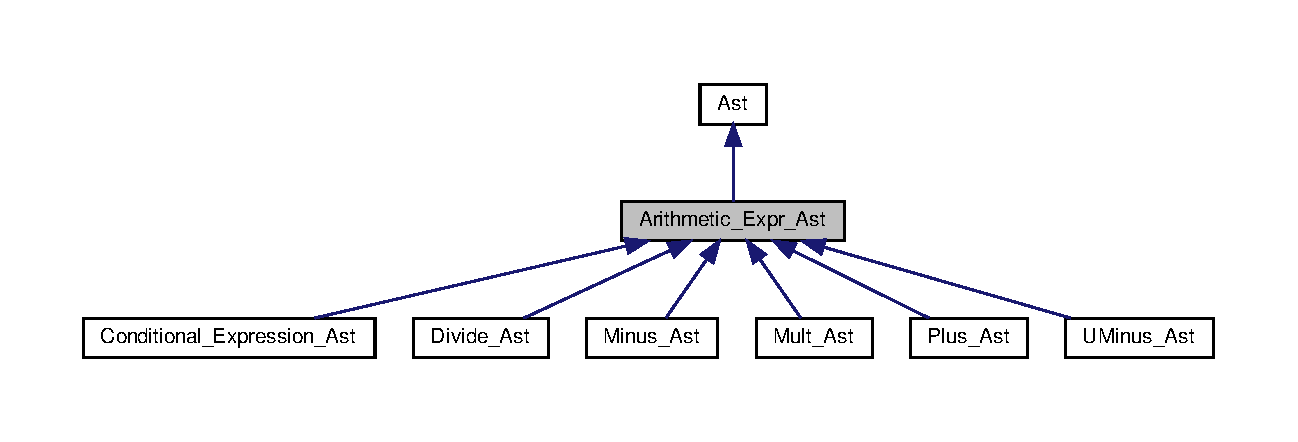
\includegraphics[width=350pt]{classArithmetic__Expr__Ast__inherit__graph}
\end{center}
\end{figure}


Collaboration diagram for Arithmetic\+\_\+\+Expr\+\_\+\+Ast\+:
\nopagebreak
\begin{figure}[H]
\begin{center}
\leavevmode
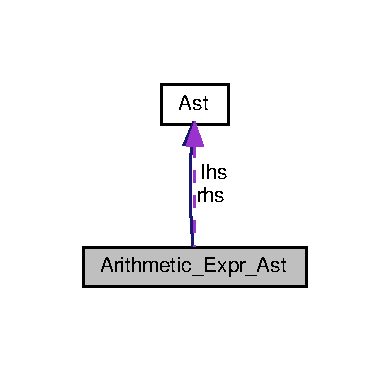
\includegraphics[width=187pt]{classArithmetic__Expr__Ast__coll__graph}
\end{center}
\end{figure}
\subsection*{Public Member Functions}
\begin{DoxyCompactItemize}
\item 
\mbox{\Hypertarget{classArithmetic__Expr__Ast_ad0ce7375a902b68a958cacda6fa3b4d5}\label{classArithmetic__Expr__Ast_ad0ce7375a902b68a958cacda6fa3b4d5}} 
Data\+\_\+\+Type {\bfseries get\+\_\+data\+\_\+type} ()
\item 
\mbox{\Hypertarget{classArithmetic__Expr__Ast_a591e5192e2f05b573d1c808015ca170b}\label{classArithmetic__Expr__Ast_a591e5192e2f05b573d1c808015ca170b}} 
void {\bfseries set\+\_\+data\+\_\+type} (Data\+\_\+\+Type dt)
\item 
\mbox{\Hypertarget{classArithmetic__Expr__Ast_ac05652b0220be526859bad95c6873df1}\label{classArithmetic__Expr__Ast_ac05652b0220be526859bad95c6873df1}} 
void {\bfseries type\+\_\+check\+\_\+ast} ()
\item 
\mbox{\Hypertarget{classArithmetic__Expr__Ast_ad3885866e66c45420689b6e469076b53}\label{classArithmetic__Expr__Ast_ad3885866e66c45420689b6e469076b53}} 
virtual void {\bfseries print\+\_\+ast} (ostream \&file\+\_\+buffer)=0
\end{DoxyCompactItemize}
\subsection*{Protected Attributes}
\begin{DoxyCompactItemize}
\item 
\mbox{\Hypertarget{classArithmetic__Expr__Ast_a1e86584c80d3bf1f1d778c86f3ab4b69}\label{classArithmetic__Expr__Ast_a1e86584c80d3bf1f1d778c86f3ab4b69}} 
\hyperlink{classAst}{Ast} $\ast$ {\bfseries lhs}
\item 
\mbox{\Hypertarget{classArithmetic__Expr__Ast_afd3b364f7d4d7df60e33b8473102bb45}\label{classArithmetic__Expr__Ast_afd3b364f7d4d7df60e33b8473102bb45}} 
\hyperlink{classAst}{Ast} $\ast$ {\bfseries rhs}
\end{DoxyCompactItemize}
\subsection*{Additional Inherited Members}


The documentation for this class was generated from the following files\+:\begin{DoxyCompactItemize}
\item 
ast.\+hh\item 
ast.\+cc\item 
type-\/checking.\+cc\end{DoxyCompactItemize}

\hypertarget{classAssignment__Ast}{}\section{Assignment\+\_\+\+Ast Class Reference}
\label{classAssignment__Ast}\index{Assignment\+\_\+\+Ast@{Assignment\+\_\+\+Ast}}


Inheritance diagram for Assignment\+\_\+\+Ast\+:
\nopagebreak
\begin{figure}[H]
\begin{center}
\leavevmode
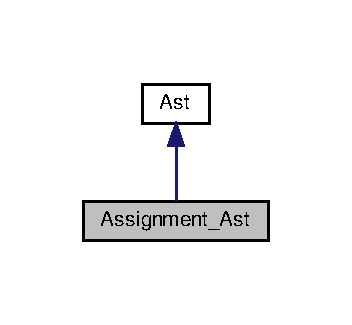
\includegraphics[width=169pt]{classAssignment__Ast__inherit__graph}
\end{center}
\end{figure}


Collaboration diagram for Assignment\+\_\+\+Ast\+:
\nopagebreak
\begin{figure}[H]
\begin{center}
\leavevmode
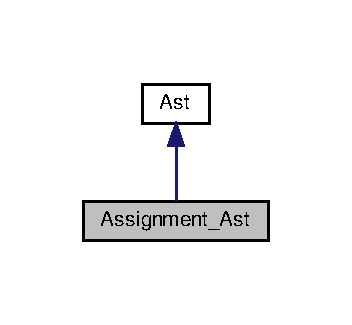
\includegraphics[width=169pt]{classAssignment__Ast__coll__graph}
\end{center}
\end{figure}
\subsection*{Public Member Functions}
\begin{DoxyCompactItemize}
\item 
\mbox{\Hypertarget{classAssignment__Ast_a318c262a2585ec46368d8062a6e00b08}\label{classAssignment__Ast_a318c262a2585ec46368d8062a6e00b08}} 
{\bfseries Assignment\+\_\+\+Ast} (\hyperlink{classAst}{Ast} $\ast$temp\+\_\+lhs, \hyperlink{classAst}{Ast} $\ast$temp\+\_\+rhs, int line)
\item 
\mbox{\Hypertarget{classAssignment__Ast_af58349349db55986abab06d642eefc83}\label{classAssignment__Ast_af58349349db55986abab06d642eefc83}} 
void {\bfseries type\+\_\+check\+\_\+ast} ()
\item 
\mbox{\Hypertarget{classAssignment__Ast_a7d828e4bdd578dea0e47ef525022900e}\label{classAssignment__Ast_a7d828e4bdd578dea0e47ef525022900e}} 
void {\bfseries print\+\_\+ast} (ostream \&file\+\_\+buffer)
\item 
\mbox{\Hypertarget{classAssignment__Ast_a03043287ac465a7db828ae758f7cc72d}\label{classAssignment__Ast_a03043287ac465a7db828ae758f7cc72d}} 
\hyperlink{classTAC__For__Ast}{T\+A\+C\+\_\+\+For\+\_\+\+Ast} $\ast$ {\bfseries gen\+\_\+tac} ()
\end{DoxyCompactItemize}
\subsection*{Additional Inherited Members}


The documentation for this class was generated from the following files\+:\begin{DoxyCompactItemize}
\item 
ast.\+hh\item 
ast.\+cc\item 
tac-\/gen.\+cc\item 
type-\/checking.\+cc\end{DoxyCompactItemize}

\hypertarget{classAst}{}\section{Ast Class Reference}
\label{classAst}\index{Ast@{Ast}}


Inheritance diagram for Ast\+:
\nopagebreak
\begin{figure}[H]
\begin{center}
\leavevmode
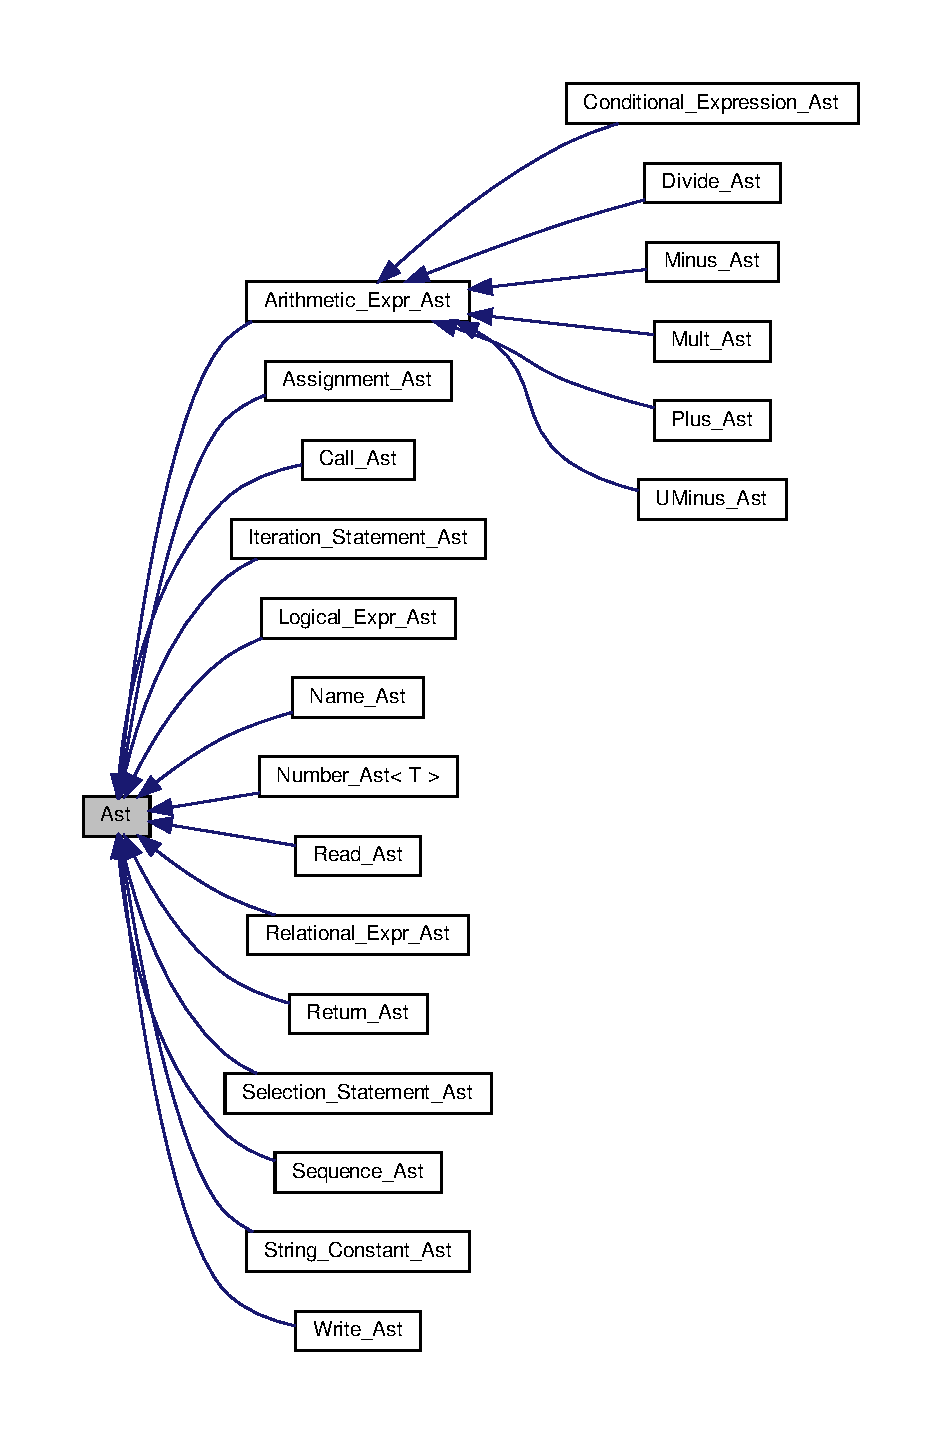
\includegraphics[width=350pt]{classAst__inherit__graph}
\end{center}
\end{figure}
\subsection*{Public Member Functions}
\begin{DoxyCompactItemize}
\item 
\mbox{\Hypertarget{classAst_a59e90c47de802634360a46095bdfb9ac}\label{classAst_a59e90c47de802634360a46095bdfb9ac}} 
virtual Data\+\_\+\+Type {\bfseries get\+\_\+data\+\_\+type} ()
\item 
\mbox{\Hypertarget{classAst_a5a8064877aa16ce098ddc75f93f55c1f}\label{classAst_a5a8064877aa16ce098ddc75f93f55c1f}} 
virtual void {\bfseries set\+\_\+data\+\_\+type} (Data\+\_\+\+Type dt)
\item 
\mbox{\Hypertarget{classAst_a7c5270909ce443f527f76d5911ebdf92}\label{classAst_a7c5270909ce443f527f76d5911ebdf92}} 
virtual bool {\bfseries is\+\_\+value\+\_\+zero} ()
\item 
\mbox{\Hypertarget{classAst_ae30169be4e52e013a5e6681cff1da803}\label{classAst_ae30169be4e52e013a5e6681cff1da803}} 
virtual void {\bfseries type\+\_\+check\+\_\+ast} ()
\item 
\mbox{\Hypertarget{classAst_acfee244438a83610c1ad31772b6e0386}\label{classAst_acfee244438a83610c1ad31772b6e0386}} 
virtual \hyperlink{classSymbol__Table__Entry}{Symbol\+\_\+\+Table\+\_\+\+Entry} \& {\bfseries get\+\_\+symbol\+\_\+entry} ()
\item 
\mbox{\Hypertarget{classAst_a98a074f3b5a6b264644b971c453ca07d}\label{classAst_a98a074f3b5a6b264644b971c453ca07d}} 
virtual void {\bfseries print\+\_\+ast} (ostream \&file\+\_\+buffer)=0
\item 
\mbox{\Hypertarget{classAst_a0f9ef33a1229580bc9b92cd831681981}\label{classAst_a0f9ef33a1229580bc9b92cd831681981}} 
virtual \hyperlink{classTAC__For__Ast}{T\+A\+C\+\_\+\+For\+\_\+\+Ast} $\ast$ {\bfseries gen\+\_\+tac} ()
\item 
\mbox{\Hypertarget{classAst_a4d6bf010ebb08c96bf163ecb13a05bca}\label{classAst_a4d6bf010ebb08c96bf163ecb13a05bca}} 
virtual T\+A\+C\+\_\+\+Op {\bfseries get\+\_\+tac\+\_\+operator\+\_\+for\+\_\+rel\+\_\+operator} ()
\end{DoxyCompactItemize}
\subsection*{Protected Member Functions}
\begin{DoxyCompactItemize}
\item 
\mbox{\Hypertarget{classAst_a202c29a1c1dca716a61bc969bb1a9733}\label{classAst_a202c29a1c1dca716a61bc969bb1a9733}} 
string {\bfseries get\+\_\+new\+\_\+label} ()
\end{DoxyCompactItemize}
\subsection*{Protected Attributes}
\begin{DoxyCompactItemize}
\item 
\mbox{\Hypertarget{classAst_a09e0a05ac8ec17d32f94f645b6a83d84}\label{classAst_a09e0a05ac8ec17d32f94f645b6a83d84}} 
Data\+\_\+\+Type {\bfseries node\+\_\+data\+\_\+type}
\item 
\mbox{\Hypertarget{classAst_abaeced57d7c8ee027f71e62d0eba22e6}\label{classAst_abaeced57d7c8ee027f71e62d0eba22e6}} 
int {\bfseries lineno}
\end{DoxyCompactItemize}
\subsection*{Static Protected Attributes}
\begin{DoxyCompactItemize}
\item 
\mbox{\Hypertarget{classAst_ad0766f2d2f39a7575c5e8210dc9aad9f}\label{classAst_ad0766f2d2f39a7575c5e8210dc9aad9f}} 
static int {\bfseries label\+Counter}
\end{DoxyCompactItemize}


The documentation for this class was generated from the following files\+:\begin{DoxyCompactItemize}
\item 
ast.\+hh\item 
ast.\+cc\item 
type-\/checking.\+cc\end{DoxyCompactItemize}

\hypertarget{classCall__Ast}{}\section{Call\+\_\+\+Ast Class Reference}
\label{classCall__Ast}\index{Call\+\_\+\+Ast@{Call\+\_\+\+Ast}}


Inheritance diagram for Call\+\_\+\+Ast\+:
\nopagebreak
\begin{figure}[H]
\begin{center}
\leavevmode
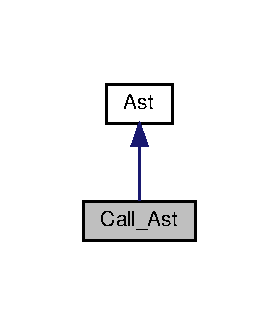
\includegraphics[width=134pt]{classCall__Ast__inherit__graph}
\end{center}
\end{figure}


Collaboration diagram for Call\+\_\+\+Ast\+:
\nopagebreak
\begin{figure}[H]
\begin{center}
\leavevmode
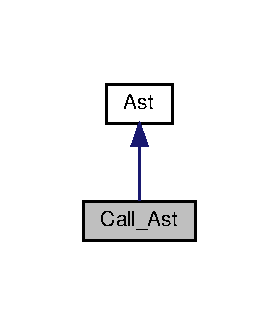
\includegraphics[width=134pt]{classCall__Ast__coll__graph}
\end{center}
\end{figure}
\subsection*{Public Member Functions}
\begin{DoxyCompactItemize}
\item 
\mbox{\Hypertarget{classCall__Ast_a9091b91b04cf1c0368baf992cef77a7a}\label{classCall__Ast_a9091b91b04cf1c0368baf992cef77a7a}} 
{\bfseries Call\+\_\+\+Ast} (string name, int line)
\item 
\mbox{\Hypertarget{classCall__Ast_aae0b807631e876325731b460b571d122}\label{classCall__Ast_aae0b807631e876325731b460b571d122}} 
Data\+\_\+\+Type {\bfseries get\+\_\+data\+\_\+type} ()
\item 
\mbox{\Hypertarget{classCall__Ast_a28cbf71b5ec6714fdd4b97e7e558acba}\label{classCall__Ast_a28cbf71b5ec6714fdd4b97e7e558acba}} 
void {\bfseries set\+\_\+register} (\hyperlink{classRegister__Descriptor}{Register\+\_\+\+Descriptor} $\ast$reg)
\item 
\mbox{\Hypertarget{classCall__Ast_add4163ec6ed31925bbc50704a14d2412}\label{classCall__Ast_add4163ec6ed31925bbc50704a14d2412}} 
void {\bfseries type\+\_\+check\+\_\+actual\+\_\+formal\+\_\+param} (\hyperlink{classSymbol__Table}{Symbol\+\_\+\+Table} \&formal\+\_\+param\+\_\+list)
\item 
\mbox{\Hypertarget{classCall__Ast_acc93a340af549158bf4efc5e1041984a}\label{classCall__Ast_acc93a340af549158bf4efc5e1041984a}} 
void {\bfseries set\+\_\+actual\+\_\+param\+\_\+list} (list$<$ \hyperlink{classAst}{Ast} $\ast$$>$ \&param\+\_\+list)
\item 
\mbox{\Hypertarget{classCall__Ast_ab0732164ac9b9dc8227c78eb9898b070}\label{classCall__Ast_ab0732164ac9b9dc8227c78eb9898b070}} 
void {\bfseries print\+\_\+ast} (ostream \&file\+\_\+buffer)
\end{DoxyCompactItemize}
\subsection*{Additional Inherited Members}


The documentation for this class was generated from the following files\+:\begin{DoxyCompactItemize}
\item 
ast.\+hh\item 
ast.\+cc\item 
type-\/checking.\+cc\end{DoxyCompactItemize}

\hypertarget{classCall__TAC__Stmt}{}\section{Call\+\_\+\+T\+A\+C\+\_\+\+Stmt Class Reference}
\label{classCall__TAC__Stmt}\index{Call\+\_\+\+T\+A\+C\+\_\+\+Stmt@{Call\+\_\+\+T\+A\+C\+\_\+\+Stmt}}


Inheritance diagram for Call\+\_\+\+T\+A\+C\+\_\+\+Stmt\+:
\nopagebreak
\begin{figure}[H]
\begin{center}
\leavevmode
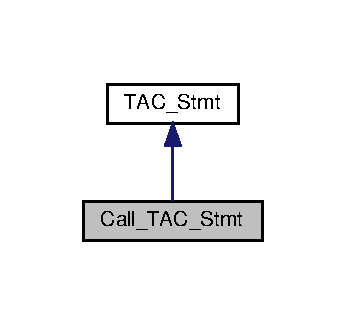
\includegraphics[width=166pt]{classCall__TAC__Stmt__inherit__graph}
\end{center}
\end{figure}


Collaboration diagram for Call\+\_\+\+T\+A\+C\+\_\+\+Stmt\+:
\nopagebreak
\begin{figure}[H]
\begin{center}
\leavevmode
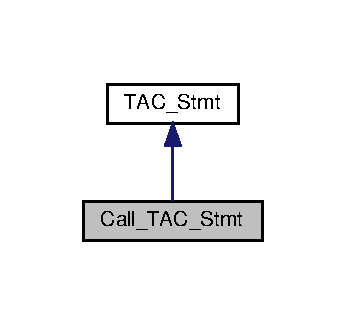
\includegraphics[width=166pt]{classCall__TAC__Stmt__coll__graph}
\end{center}
\end{figure}
\subsection*{Public Member Functions}
\begin{DoxyCompactItemize}
\item 
\mbox{\Hypertarget{classCall__TAC__Stmt_af71e8f7154076070f38a1238fb5a8229}\label{classCall__TAC__Stmt_af71e8f7154076070f38a1238fb5a8229}} 
{\bfseries Call\+\_\+\+T\+A\+C\+\_\+\+Stmt} (\hyperlink{classTAC__Opd}{T\+A\+C\+\_\+\+Opd} $\ast$opd1, \hyperlink{classTAC__Opd}{T\+A\+C\+\_\+\+Opd} $\ast$result)
\item 
\mbox{\Hypertarget{classCall__TAC__Stmt_a04b24421ef58a80b06d7a1bd5ff6d4a5}\label{classCall__TAC__Stmt_a04b24421ef58a80b06d7a1bd5ff6d4a5}} 
\hyperlink{classTAC__Opd}{T\+A\+C\+\_\+\+Opd} $\ast$ {\bfseries get\+\_\+opd1} ()
\item 
\mbox{\Hypertarget{classCall__TAC__Stmt_a28c9365b1f1146f3f8120b067a8ae6db}\label{classCall__TAC__Stmt_a28c9365b1f1146f3f8120b067a8ae6db}} 
\hyperlink{classTAC__Opd}{T\+A\+C\+\_\+\+Opd} $\ast$ {\bfseries get\+\_\+result} ()
\item 
\mbox{\Hypertarget{classCall__TAC__Stmt_ab9a2475b55b6ba77afec39ea785ce7bf}\label{classCall__TAC__Stmt_ab9a2475b55b6ba77afec39ea785ce7bf}} 
list$<$ \hyperlink{classTAC__Opd}{T\+A\+C\+\_\+\+Opd} $\ast$ $>$ {\bfseries get\+\_\+actual\+\_\+param\+\_\+list} ()
\item 
\mbox{\Hypertarget{classCall__TAC__Stmt_af9269c7a28251eb0fde2ca1d801674f6}\label{classCall__TAC__Stmt_af9269c7a28251eb0fde2ca1d801674f6}} 
void {\bfseries set\+\_\+opd1} (\hyperlink{classTAC__Opd}{T\+A\+C\+\_\+\+Opd} $\ast$opd)
\item 
\mbox{\Hypertarget{classCall__TAC__Stmt_ae7ab3cde1e0f1f5288fb71932cbb2bc4}\label{classCall__TAC__Stmt_ae7ab3cde1e0f1f5288fb71932cbb2bc4}} 
void {\bfseries set\+\_\+result} (\hyperlink{classTAC__Opd}{T\+A\+C\+\_\+\+Opd} $\ast$opd)
\item 
\mbox{\Hypertarget{classCall__TAC__Stmt_aa2ab0635b937cc9b6066ede61fd48aed}\label{classCall__TAC__Stmt_aa2ab0635b937cc9b6066ede61fd48aed}} 
void {\bfseries set\+\_\+actual\+\_\+param\+\_\+list} (list$<$ \hyperlink{classTAC__Opd}{T\+A\+C\+\_\+\+Opd} $\ast$$>$ apl)
\item 
\mbox{\Hypertarget{classCall__TAC__Stmt_a24a3894a1d2ec4c3ea963565180d7fd8}\label{classCall__TAC__Stmt_a24a3894a1d2ec4c3ea963565180d7fd8}} 
void {\bfseries print\+\_\+tac\+\_\+stmt} (ostream \&file\+\_\+buffer)
\end{DoxyCompactItemize}
\subsection*{Additional Inherited Members}


The documentation for this class was generated from the following file\+:\begin{DoxyCompactItemize}
\item 
tac.\+hh\end{DoxyCompactItemize}

\hypertarget{classCompute__RTL__Stmt}{}\section{Compute\+\_\+\+R\+T\+L\+\_\+\+Stmt Class Reference}
\label{classCompute__RTL__Stmt}\index{Compute\+\_\+\+R\+T\+L\+\_\+\+Stmt@{Compute\+\_\+\+R\+T\+L\+\_\+\+Stmt}}


Inheritance diagram for Compute\+\_\+\+R\+T\+L\+\_\+\+Stmt\+:
\nopagebreak
\begin{figure}[H]
\begin{center}
\leavevmode
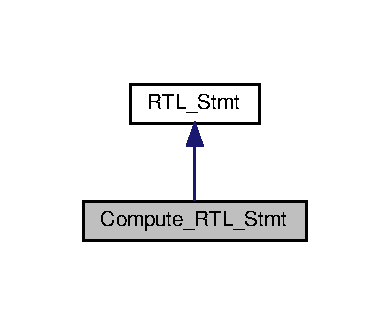
\includegraphics[width=187pt]{classCompute__RTL__Stmt__inherit__graph}
\end{center}
\end{figure}


Collaboration diagram for Compute\+\_\+\+R\+T\+L\+\_\+\+Stmt\+:
\nopagebreak
\begin{figure}[H]
\begin{center}
\leavevmode
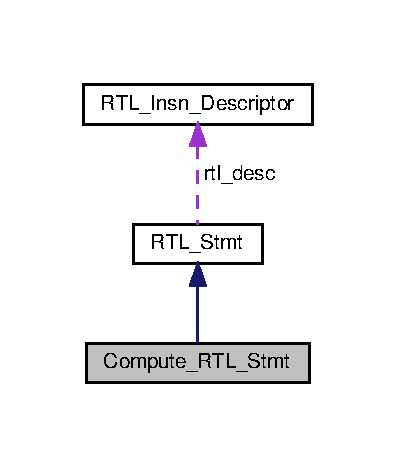
\includegraphics[width=190pt]{classCompute__RTL__Stmt__coll__graph}
\end{center}
\end{figure}
\subsection*{Public Member Functions}
\begin{DoxyCompactItemize}
\item 
\mbox{\Hypertarget{classCompute__RTL__Stmt_ab75c03cb392f5cd6ab91b8a88630c3f3}\label{classCompute__RTL__Stmt_ab75c03cb392f5cd6ab91b8a88630c3f3}} 
{\bfseries Compute\+\_\+\+R\+T\+L\+\_\+\+Stmt} (R\+T\+L\+\_\+\+Op inst\+\_\+op, \hyperlink{classRTL__Opd}{R\+T\+L\+\_\+\+Opd} $\ast$opd1, \hyperlink{classRTL__Opd}{R\+T\+L\+\_\+\+Opd} $\ast$opd2, \hyperlink{classRTL__Opd}{R\+T\+L\+\_\+\+Opd} $\ast$result)
\item 
\mbox{\Hypertarget{classCompute__RTL__Stmt_a9bd759f30ff8e04990796b2a136897ee}\label{classCompute__RTL__Stmt_a9bd759f30ff8e04990796b2a136897ee}} 
\hyperlink{classCompute__RTL__Stmt}{Compute\+\_\+\+R\+T\+L\+\_\+\+Stmt} \& {\bfseries operator=} (const \hyperlink{classCompute__RTL__Stmt}{Compute\+\_\+\+R\+T\+L\+\_\+\+Stmt} \&rhs)
\item 
\mbox{\Hypertarget{classCompute__RTL__Stmt_a9920d7823fd5d5c71c016ee39c081beb}\label{classCompute__RTL__Stmt_a9920d7823fd5d5c71c016ee39c081beb}} 
\hyperlink{classRTL__Insn__Descriptor}{R\+T\+L\+\_\+\+Insn\+\_\+\+Descriptor} \& {\bfseries get\+\_\+inst\+\_\+op\+\_\+of\+\_\+rtl\+\_\+stmt} ()
\item 
\mbox{\Hypertarget{classCompute__RTL__Stmt_a534fc4122c89223060b7e9f5238daf84}\label{classCompute__RTL__Stmt_a534fc4122c89223060b7e9f5238daf84}} 
\hyperlink{classRTL__Opd}{R\+T\+L\+\_\+\+Opd} $\ast$ {\bfseries get\+\_\+opd1} ()
\item 
\mbox{\Hypertarget{classCompute__RTL__Stmt_a2f37ebccfe81fa33558dd185afd94973}\label{classCompute__RTL__Stmt_a2f37ebccfe81fa33558dd185afd94973}} 
void {\bfseries set\+\_\+opd1} (\hyperlink{classRTL__Opd}{R\+T\+L\+\_\+\+Opd} $\ast$io)
\item 
\mbox{\Hypertarget{classCompute__RTL__Stmt_af87454a3a2f02b3416c5e4e818f70a17}\label{classCompute__RTL__Stmt_af87454a3a2f02b3416c5e4e818f70a17}} 
\hyperlink{classRTL__Opd}{R\+T\+L\+\_\+\+Opd} $\ast$ {\bfseries get\+\_\+opd2} ()
\item 
\mbox{\Hypertarget{classCompute__RTL__Stmt_ab93a1f9cd8d50b168bdfa58708f1d917}\label{classCompute__RTL__Stmt_ab93a1f9cd8d50b168bdfa58708f1d917}} 
void {\bfseries set\+\_\+opd2} (\hyperlink{classRTL__Opd}{R\+T\+L\+\_\+\+Opd} $\ast$io)
\item 
\mbox{\Hypertarget{classCompute__RTL__Stmt_a6d9de0ad00db8a49fd285686377e3e42}\label{classCompute__RTL__Stmt_a6d9de0ad00db8a49fd285686377e3e42}} 
\hyperlink{classRTL__Opd}{R\+T\+L\+\_\+\+Opd} $\ast$ {\bfseries get\+\_\+result} ()
\item 
\mbox{\Hypertarget{classCompute__RTL__Stmt_a1fa7508ac3fd34bfd1341cce15e3a199}\label{classCompute__RTL__Stmt_a1fa7508ac3fd34bfd1341cce15e3a199}} 
void {\bfseries set\+\_\+result} (\hyperlink{classRTL__Opd}{R\+T\+L\+\_\+\+Opd} $\ast$io)
\item 
\mbox{\Hypertarget{classCompute__RTL__Stmt_aac7caa0b0d6b8f46ef1b605154bb1b16}\label{classCompute__RTL__Stmt_aac7caa0b0d6b8f46ef1b605154bb1b16}} 
void {\bfseries print\+\_\+rtl\+\_\+stmt} (ostream \&file\+\_\+buffer)
\item 
\mbox{\Hypertarget{classCompute__RTL__Stmt_ad10729ddf06d2ddf5beadd7e1ee2d888}\label{classCompute__RTL__Stmt_ad10729ddf06d2ddf5beadd7e1ee2d888}} 
void {\bfseries print\+\_\+assembly} (ostream \&file\+\_\+buffer)
\end{DoxyCompactItemize}
\subsection*{Additional Inherited Members}


The documentation for this class was generated from the following files\+:\begin{DoxyCompactItemize}
\item 
rtl.\+hh\item 
rtl.\+cc\end{DoxyCompactItemize}

\hypertarget{classCompute__TAC__Stmt}{}\section{Compute\+\_\+\+T\+A\+C\+\_\+\+Stmt Class Reference}
\label{classCompute__TAC__Stmt}\index{Compute\+\_\+\+T\+A\+C\+\_\+\+Stmt@{Compute\+\_\+\+T\+A\+C\+\_\+\+Stmt}}


{\ttfamily \#include $<$tac.\+hh$>$}



Inheritance diagram for Compute\+\_\+\+T\+A\+C\+\_\+\+Stmt\+:
\nopagebreak
\begin{figure}[H]
\begin{center}
\leavevmode
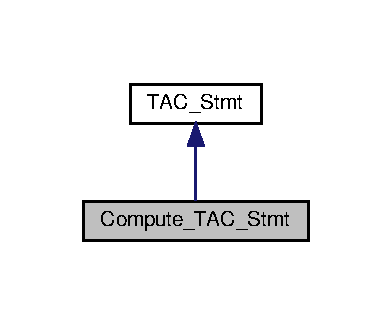
\includegraphics[width=188pt]{classCompute__TAC__Stmt__inherit__graph}
\end{center}
\end{figure}


Collaboration diagram for Compute\+\_\+\+T\+A\+C\+\_\+\+Stmt\+:
\nopagebreak
\begin{figure}[H]
\begin{center}
\leavevmode
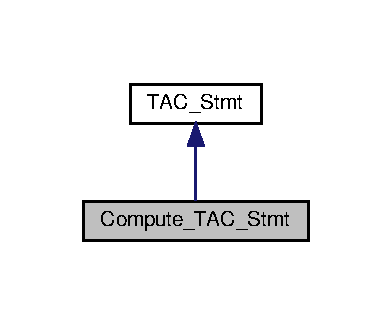
\includegraphics[width=188pt]{classCompute__TAC__Stmt__coll__graph}
\end{center}
\end{figure}
\subsection*{Public Member Functions}
\begin{DoxyCompactItemize}
\item 
\mbox{\Hypertarget{classCompute__TAC__Stmt_a62be94e3aeef3deab5c9ea2500fd2b70}\label{classCompute__TAC__Stmt_a62be94e3aeef3deab5c9ea2500fd2b70}} 
{\bfseries Compute\+\_\+\+T\+A\+C\+\_\+\+Stmt} (T\+A\+C\+\_\+\+Op op, \hyperlink{classTAC__Opd}{T\+A\+C\+\_\+\+Opd} $\ast$opd1, \hyperlink{classTAC__Opd}{T\+A\+C\+\_\+\+Opd} $\ast$opd2, \hyperlink{classTAC__Opd}{T\+A\+C\+\_\+\+Opd} $\ast$result, Data\+\_\+\+Type dt)
\item 
\mbox{\Hypertarget{classCompute__TAC__Stmt_ade06a4723460836ec31d40c1067b7e68}\label{classCompute__TAC__Stmt_ade06a4723460836ec31d40c1067b7e68}} 
R\+T\+L\+\_\+\+Op {\bfseries get\+\_\+rtl\+\_\+operator\+\_\+for\+\_\+tac\+\_\+operator} ()
\item 
\mbox{\Hypertarget{classCompute__TAC__Stmt_aefd7a18e6103b65b86a05d0721d6f33b}\label{classCompute__TAC__Stmt_aefd7a18e6103b65b86a05d0721d6f33b}} 
\hyperlink{classTAC__Opd}{T\+A\+C\+\_\+\+Opd} $\ast$ {\bfseries get\+\_\+opd1} ()
\item 
\mbox{\Hypertarget{classCompute__TAC__Stmt_a09efa8ce58065a9d4d559ffbb30c8f87}\label{classCompute__TAC__Stmt_a09efa8ce58065a9d4d559ffbb30c8f87}} 
\hyperlink{classTAC__Opd}{T\+A\+C\+\_\+\+Opd} $\ast$ {\bfseries get\+\_\+opd2} ()
\item 
\mbox{\Hypertarget{classCompute__TAC__Stmt_a2fac5f3d6b58fecc84c50c83518757a8}\label{classCompute__TAC__Stmt_a2fac5f3d6b58fecc84c50c83518757a8}} 
\hyperlink{classTAC__Opd}{T\+A\+C\+\_\+\+Opd} $\ast$ {\bfseries get\+\_\+result} ()
\item 
\mbox{\Hypertarget{classCompute__TAC__Stmt_a292d8812461a47c8f3250aeeaae0de7e}\label{classCompute__TAC__Stmt_a292d8812461a47c8f3250aeeaae0de7e}} 
void {\bfseries set\+\_\+opd1} (\hyperlink{classTAC__Opd}{T\+A\+C\+\_\+\+Opd} $\ast$opd)
\item 
\mbox{\Hypertarget{classCompute__TAC__Stmt_ab375f421aee8d75d3ff40529d39f770b}\label{classCompute__TAC__Stmt_ab375f421aee8d75d3ff40529d39f770b}} 
void {\bfseries set\+\_\+opd2} (\hyperlink{classTAC__Opd}{T\+A\+C\+\_\+\+Opd} $\ast$opd)
\item 
\mbox{\Hypertarget{classCompute__TAC__Stmt_a2570e55808af6179056afedcc570d8b4}\label{classCompute__TAC__Stmt_a2570e55808af6179056afedcc570d8b4}} 
void {\bfseries set\+\_\+result} (\hyperlink{classTAC__Opd}{T\+A\+C\+\_\+\+Opd} $\ast$res)
\item 
\mbox{\Hypertarget{classCompute__TAC__Stmt_a656bd44d06df4de10abe2836d801bde1}\label{classCompute__TAC__Stmt_a656bd44d06df4de10abe2836d801bde1}} 
Data\+\_\+\+Type {\bfseries get\+\_\+data\+\_\+type} ()
\item 
\mbox{\Hypertarget{classCompute__TAC__Stmt_ae46b480642729802bc78ed3bbe6bb05c}\label{classCompute__TAC__Stmt_ae46b480642729802bc78ed3bbe6bb05c}} 
\hyperlink{classRTL__For__TAC}{R\+T\+L\+\_\+\+For\+\_\+\+T\+AC} \& {\bfseries gen\+\_\+rtl} ()
\item 
\mbox{\Hypertarget{classCompute__TAC__Stmt_ae3781aa58f671f1a330ec1151c927ab3}\label{classCompute__TAC__Stmt_ae3781aa58f671f1a330ec1151c927ab3}} 
void {\bfseries print\+\_\+tac\+\_\+stmt} (ostream \&file\+\_\+buffer)
\end{DoxyCompactItemize}
\subsection*{Additional Inherited Members}


\subsection{Detailed Description}
T\+AC Compute Statement //////////////////////////////////// Arithmetic operations\+: add\+\_\+3a, sub\+\_\+3a, mult\+\_\+3a, div\+\_\+a, uminus\+\_\+3a //////////////////////// Logical operations\+: and\+\_\+3a, or\+\_\+3a, not\+\_\+3a ////////////////////////////// Comparison operations\+: lt\+\_\+3a, leq\+\_\+3a, gt\+\_\+3a, geq\+\_\+3a, eq\+\_\+3a, neq\+\_\+3a ////////////////////////////// 

The documentation for this class was generated from the following files\+:\begin{DoxyCompactItemize}
\item 
tac.\+hh\item 
rtl-\/gen.\+cc\item 
tac.\+cc\end{DoxyCompactItemize}

\hypertarget{classConditional__Expression__Ast}{}\section{Conditional\+\_\+\+Expression\+\_\+\+Ast Class Reference}
\label{classConditional__Expression__Ast}\index{Conditional\+\_\+\+Expression\+\_\+\+Ast@{Conditional\+\_\+\+Expression\+\_\+\+Ast}}


Inheritance diagram for Conditional\+\_\+\+Expression\+\_\+\+Ast\+:
\nopagebreak
\begin{figure}[H]
\begin{center}
\leavevmode
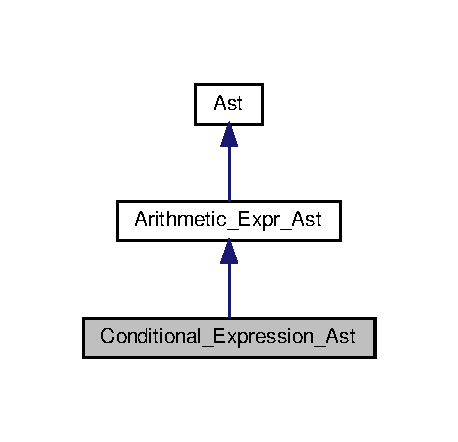
\includegraphics[width=220pt]{classConditional__Expression__Ast__inherit__graph}
\end{center}
\end{figure}


Collaboration diagram for Conditional\+\_\+\+Expression\+\_\+\+Ast\+:
\nopagebreak
\begin{figure}[H]
\begin{center}
\leavevmode
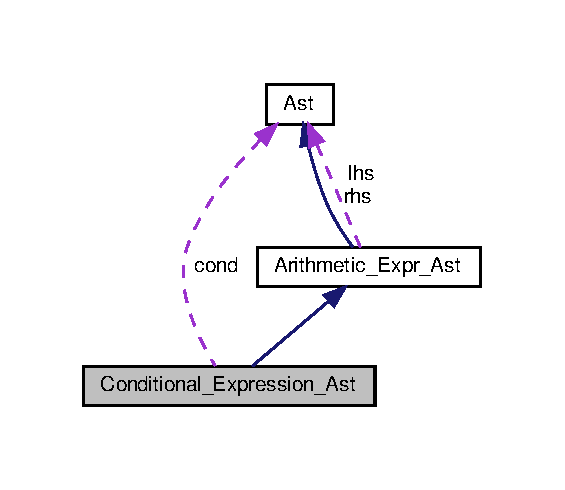
\includegraphics[width=271pt]{classConditional__Expression__Ast__coll__graph}
\end{center}
\end{figure}
\subsection*{Public Member Functions}
\begin{DoxyCompactItemize}
\item 
\mbox{\Hypertarget{classConditional__Expression__Ast_aa6b12af384f8de1ac623289f1a00456c}\label{classConditional__Expression__Ast_aa6b12af384f8de1ac623289f1a00456c}} 
{\bfseries Conditional\+\_\+\+Expression\+\_\+\+Ast} (\hyperlink{classAst}{Ast} $\ast$cond, \hyperlink{classAst}{Ast} $\ast$l, \hyperlink{classAst}{Ast} $\ast$r, int line)
\item 
\mbox{\Hypertarget{classConditional__Expression__Ast_abc60e586a729c80b6ec05f01eac5766f}\label{classConditional__Expression__Ast_abc60e586a729c80b6ec05f01eac5766f}} 
void {\bfseries print\+\_\+ast} (ostream \&file\+\_\+buffer)
\item 
\mbox{\Hypertarget{classConditional__Expression__Ast_afae8029a346410e02f29be9064080d72}\label{classConditional__Expression__Ast_afae8029a346410e02f29be9064080d72}} 
\hyperlink{classTAC__For__Ast}{T\+A\+C\+\_\+\+For\+\_\+\+Ast} $\ast$ {\bfseries gen\+\_\+tac} ()
\end{DoxyCompactItemize}
\subsection*{Protected Attributes}
\begin{DoxyCompactItemize}
\item 
\mbox{\Hypertarget{classConditional__Expression__Ast_afd90dd444308073ed4f801f3e67e5f08}\label{classConditional__Expression__Ast_afd90dd444308073ed4f801f3e67e5f08}} 
\hyperlink{classAst}{Ast} $\ast$ {\bfseries cond}
\end{DoxyCompactItemize}
\subsection*{Additional Inherited Members}


The documentation for this class was generated from the following files\+:\begin{DoxyCompactItemize}
\item 
ast.\+hh\item 
ast.\+cc\item 
tac-\/gen.\+cc\end{DoxyCompactItemize}

\hypertarget{classControl__Flow__RTL__Stmt}{}\section{Control\+\_\+\+Flow\+\_\+\+R\+T\+L\+\_\+\+Stmt Class Reference}
\label{classControl__Flow__RTL__Stmt}\index{Control\+\_\+\+Flow\+\_\+\+R\+T\+L\+\_\+\+Stmt@{Control\+\_\+\+Flow\+\_\+\+R\+T\+L\+\_\+\+Stmt}}


Inheritance diagram for Control\+\_\+\+Flow\+\_\+\+R\+T\+L\+\_\+\+Stmt\+:
\nopagebreak
\begin{figure}[H]
\begin{center}
\leavevmode
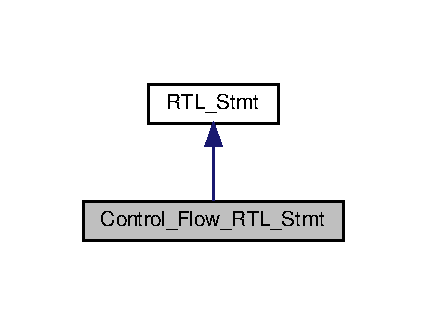
\includegraphics[width=205pt]{classControl__Flow__RTL__Stmt__inherit__graph}
\end{center}
\end{figure}


Collaboration diagram for Control\+\_\+\+Flow\+\_\+\+R\+T\+L\+\_\+\+Stmt\+:
\nopagebreak
\begin{figure}[H]
\begin{center}
\leavevmode
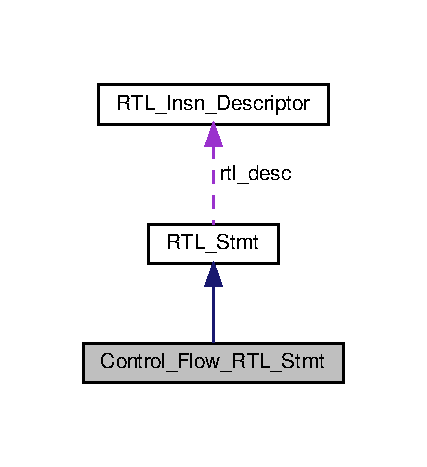
\includegraphics[width=205pt]{classControl__Flow__RTL__Stmt__coll__graph}
\end{center}
\end{figure}
\subsection*{Public Member Functions}
\begin{DoxyCompactItemize}
\item 
\mbox{\Hypertarget{classControl__Flow__RTL__Stmt_a8dbd351c9608f6e0ce5f1483dface410}\label{classControl__Flow__RTL__Stmt_a8dbd351c9608f6e0ce5f1483dface410}} 
{\bfseries Control\+\_\+\+Flow\+\_\+\+R\+T\+L\+\_\+\+Stmt} (R\+T\+L\+\_\+\+Op op, \hyperlink{classRTL__Opd}{R\+T\+L\+\_\+\+Opd} $\ast$o1, \hyperlink{classRTL__Opd}{R\+T\+L\+\_\+\+Opd} $\ast$o2, string label, int size=0)
\item 
\mbox{\Hypertarget{classControl__Flow__RTL__Stmt_a3b70665d57786a51f55cc2c8ea7a7212}\label{classControl__Flow__RTL__Stmt_a3b70665d57786a51f55cc2c8ea7a7212}} 
\hyperlink{classControl__Flow__RTL__Stmt}{Control\+\_\+\+Flow\+\_\+\+R\+T\+L\+\_\+\+Stmt} \& {\bfseries operator=} (const \hyperlink{classControl__Flow__RTL__Stmt}{Control\+\_\+\+Flow\+\_\+\+R\+T\+L\+\_\+\+Stmt} \&rhs)
\item 
\mbox{\Hypertarget{classControl__Flow__RTL__Stmt_a53c419f41cf26da959bc7ed0829e1c66}\label{classControl__Flow__RTL__Stmt_a53c419f41cf26da959bc7ed0829e1c66}} 
\hyperlink{classRTL__Insn__Descriptor}{R\+T\+L\+\_\+\+Insn\+\_\+\+Descriptor} \& {\bfseries get\+\_\+inst\+\_\+op\+\_\+of\+\_\+rtl\+\_\+stmt} ()
\item 
\mbox{\Hypertarget{classControl__Flow__RTL__Stmt_add3d591875dc85596089706b1238e3e8}\label{classControl__Flow__RTL__Stmt_add3d591875dc85596089706b1238e3e8}} 
\hyperlink{classRTL__Opd}{R\+T\+L\+\_\+\+Opd} $\ast$ {\bfseries get\+\_\+opd1} ()
\item 
\mbox{\Hypertarget{classControl__Flow__RTL__Stmt_af8a5dffc7e6b6046c85e0b98a009912f}\label{classControl__Flow__RTL__Stmt_af8a5dffc7e6b6046c85e0b98a009912f}} 
void {\bfseries set\+\_\+opd1} (\hyperlink{classRTL__Opd}{R\+T\+L\+\_\+\+Opd} $\ast$io)
\item 
\mbox{\Hypertarget{classControl__Flow__RTL__Stmt_a190db8d9cf682fd37c8cbbc98b25ad47}\label{classControl__Flow__RTL__Stmt_a190db8d9cf682fd37c8cbbc98b25ad47}} 
\hyperlink{classRTL__Opd}{R\+T\+L\+\_\+\+Opd} $\ast$ {\bfseries get\+\_\+opd2} ()
\item 
\mbox{\Hypertarget{classControl__Flow__RTL__Stmt_ac56daf2360807d006082ae052d3bf9c7}\label{classControl__Flow__RTL__Stmt_ac56daf2360807d006082ae052d3bf9c7}} 
void {\bfseries set\+\_\+opd2} (\hyperlink{classRTL__Opd}{R\+T\+L\+\_\+\+Opd} $\ast$io)
\item 
\mbox{\Hypertarget{classControl__Flow__RTL__Stmt_a3ea5ab369e49b356ef01136c8591c1ef}\label{classControl__Flow__RTL__Stmt_a3ea5ab369e49b356ef01136c8591c1ef}} 
string {\bfseries get\+\_\+\+Offset} ()
\item 
\mbox{\Hypertarget{classControl__Flow__RTL__Stmt_adeb4805b9ed2b66688e5ac62b645c278}\label{classControl__Flow__RTL__Stmt_adeb4805b9ed2b66688e5ac62b645c278}} 
void {\bfseries set\+\_\+\+Offset} (string label)
\item 
\mbox{\Hypertarget{classControl__Flow__RTL__Stmt_a779b5906f7107b474bf1ccdee671a5e1}\label{classControl__Flow__RTL__Stmt_a779b5906f7107b474bf1ccdee671a5e1}} 
void {\bfseries print\+\_\+rtl\+\_\+stmt} (ostream \&file\+\_\+buffer)
\item 
\mbox{\Hypertarget{classControl__Flow__RTL__Stmt_a08cc553b4740c0aeaa82d247b969803a}\label{classControl__Flow__RTL__Stmt_a08cc553b4740c0aeaa82d247b969803a}} 
void {\bfseries print\+\_\+assembly} (ostream \&file\+\_\+buffer)
\end{DoxyCompactItemize}
\subsection*{Additional Inherited Members}


The documentation for this class was generated from the following files\+:\begin{DoxyCompactItemize}
\item 
rtl.\+hh\item 
rtl.\+cc\end{DoxyCompactItemize}

\hypertarget{classCopy__TAC__Stmt}{}\section{Copy\+\_\+\+T\+A\+C\+\_\+\+Stmt Class Reference}
\label{classCopy__TAC__Stmt}\index{Copy\+\_\+\+T\+A\+C\+\_\+\+Stmt@{Copy\+\_\+\+T\+A\+C\+\_\+\+Stmt}}


Inheritance diagram for Copy\+\_\+\+T\+A\+C\+\_\+\+Stmt\+:
\nopagebreak
\begin{figure}[H]
\begin{center}
\leavevmode
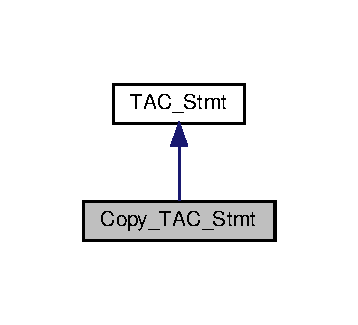
\includegraphics[width=172pt]{classCopy__TAC__Stmt__inherit__graph}
\end{center}
\end{figure}


Collaboration diagram for Copy\+\_\+\+T\+A\+C\+\_\+\+Stmt\+:
\nopagebreak
\begin{figure}[H]
\begin{center}
\leavevmode
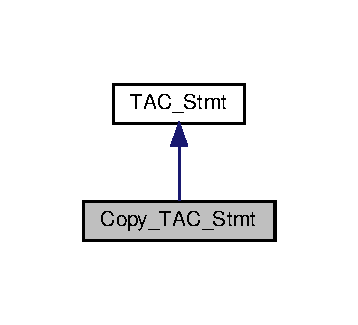
\includegraphics[width=172pt]{classCopy__TAC__Stmt__coll__graph}
\end{center}
\end{figure}
\subsection*{Public Member Functions}
\begin{DoxyCompactItemize}
\item 
\mbox{\Hypertarget{classCopy__TAC__Stmt_a0d220b873236ccfaa36817d0b92194e1}\label{classCopy__TAC__Stmt_a0d220b873236ccfaa36817d0b92194e1}} 
{\bfseries Copy\+\_\+\+T\+A\+C\+\_\+\+Stmt} (\hyperlink{classTAC__Opd}{T\+A\+C\+\_\+\+Opd} $\ast$lval, \hyperlink{classTAC__Opd}{T\+A\+C\+\_\+\+Opd} $\ast$rval)
\item 
\mbox{\Hypertarget{classCopy__TAC__Stmt_ac9ad0c26b1c3a67ed424cf452a46363c}\label{classCopy__TAC__Stmt_ac9ad0c26b1c3a67ed424cf452a46363c}} 
\hyperlink{classTAC__Opd}{T\+A\+C\+\_\+\+Opd} $\ast$ {\bfseries get\+\_\+opd1} ()
\item 
\mbox{\Hypertarget{classCopy__TAC__Stmt_a85feb421fc1104ad32cc691d764adcfd}\label{classCopy__TAC__Stmt_a85feb421fc1104ad32cc691d764adcfd}} 
\hyperlink{classTAC__Opd}{T\+A\+C\+\_\+\+Opd} $\ast$ {\bfseries get\+\_\+result} ()
\item 
\mbox{\Hypertarget{classCopy__TAC__Stmt_ab2d3aed756b96c0eefa529e956dc83cb}\label{classCopy__TAC__Stmt_ab2d3aed756b96c0eefa529e956dc83cb}} 
void {\bfseries set\+\_\+opd1} (\hyperlink{classTAC__Opd}{T\+A\+C\+\_\+\+Opd} $\ast$opd)
\item 
\mbox{\Hypertarget{classCopy__TAC__Stmt_a5415734a3cb36d2407a9e0b13d96eda6}\label{classCopy__TAC__Stmt_a5415734a3cb36d2407a9e0b13d96eda6}} 
void {\bfseries set\+\_\+result} (\hyperlink{classTAC__Opd}{T\+A\+C\+\_\+\+Opd} $\ast$res)
\item 
\mbox{\Hypertarget{classCopy__TAC__Stmt_ad42a9d258277ca20846ffc141cd56392}\label{classCopy__TAC__Stmt_ad42a9d258277ca20846ffc141cd56392}} 
\hyperlink{classRTL__For__TAC}{R\+T\+L\+\_\+\+For\+\_\+\+T\+AC} \& {\bfseries gen\+\_\+rtl} ()
\item 
\mbox{\Hypertarget{classCopy__TAC__Stmt_a83fcec2bcfc0ed3d45e0357154482f96}\label{classCopy__TAC__Stmt_a83fcec2bcfc0ed3d45e0357154482f96}} 
void {\bfseries print\+\_\+tac\+\_\+stmt} (ostream \&file\+\_\+buffer)
\end{DoxyCompactItemize}
\subsection*{Additional Inherited Members}


The documentation for this class was generated from the following files\+:\begin{DoxyCompactItemize}
\item 
tac.\+hh\item 
rtl-\/gen.\+cc\item 
tac.\+cc\end{DoxyCompactItemize}

\hypertarget{classDivide__Ast}{}\section{Divide\+\_\+\+Ast Class Reference}
\label{classDivide__Ast}\index{Divide\+\_\+\+Ast@{Divide\+\_\+\+Ast}}


Inheritance diagram for Divide\+\_\+\+Ast\+:
\nopagebreak
\begin{figure}[H]
\begin{center}
\leavevmode
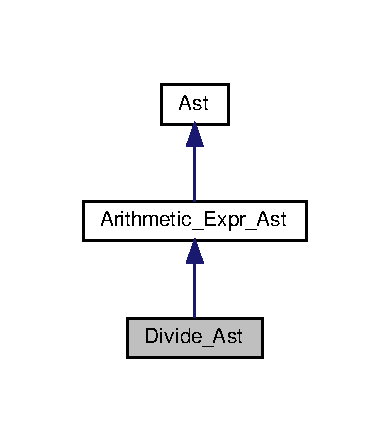
\includegraphics[width=187pt]{classDivide__Ast__inherit__graph}
\end{center}
\end{figure}


Collaboration diagram for Divide\+\_\+\+Ast\+:
\nopagebreak
\begin{figure}[H]
\begin{center}
\leavevmode
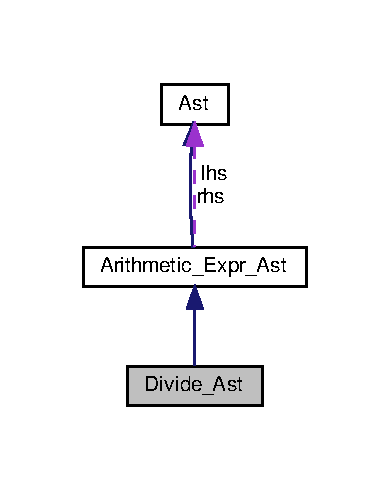
\includegraphics[width=187pt]{classDivide__Ast__coll__graph}
\end{center}
\end{figure}
\subsection*{Public Member Functions}
\begin{DoxyCompactItemize}
\item 
\mbox{\Hypertarget{classDivide__Ast_a4ee6fe5bbb61edccf3e8e2e3fc2d6d5f}\label{classDivide__Ast_a4ee6fe5bbb61edccf3e8e2e3fc2d6d5f}} 
{\bfseries Divide\+\_\+\+Ast} (\hyperlink{classAst}{Ast} $\ast$l, \hyperlink{classAst}{Ast} $\ast$r, int line)
\item 
\mbox{\Hypertarget{classDivide__Ast_abe370e59efdbbbd7b8afb2d99fbbe49b}\label{classDivide__Ast_abe370e59efdbbbd7b8afb2d99fbbe49b}} 
void {\bfseries print\+\_\+ast} (ostream \&file\+\_\+buffer)
\item 
\mbox{\Hypertarget{classDivide__Ast_a69f4bf0a7110a0ebe85292cfcf4f6734}\label{classDivide__Ast_a69f4bf0a7110a0ebe85292cfcf4f6734}} 
\hyperlink{classTAC__For__Ast}{T\+A\+C\+\_\+\+For\+\_\+\+Ast} $\ast$ {\bfseries gen\+\_\+tac} ()
\end{DoxyCompactItemize}
\subsection*{Additional Inherited Members}


The documentation for this class was generated from the following files\+:\begin{DoxyCompactItemize}
\item 
ast.\+hh\item 
ast.\+cc\item 
tac-\/gen.\+cc\end{DoxyCompactItemize}

\hypertarget{classDouble__Const__Opd}{}\section{Double\+\_\+\+Const\+\_\+\+Opd Class Reference}
\label{classDouble__Const__Opd}\index{Double\+\_\+\+Const\+\_\+\+Opd@{Double\+\_\+\+Const\+\_\+\+Opd}}


Inheritance diagram for Double\+\_\+\+Const\+\_\+\+Opd\+:
\nopagebreak
\begin{figure}[H]
\begin{center}
\leavevmode
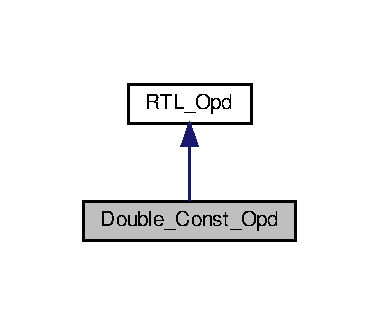
\includegraphics[width=182pt]{classDouble__Const__Opd__inherit__graph}
\end{center}
\end{figure}


Collaboration diagram for Double\+\_\+\+Const\+\_\+\+Opd\+:
\nopagebreak
\begin{figure}[H]
\begin{center}
\leavevmode
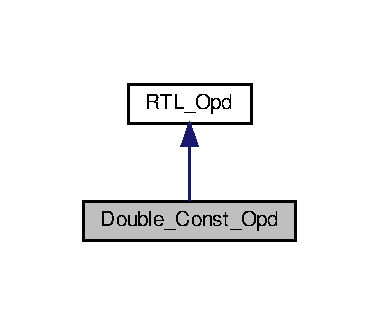
\includegraphics[width=182pt]{classDouble__Const__Opd__coll__graph}
\end{center}
\end{figure}
\subsection*{Public Member Functions}
\begin{DoxyCompactItemize}
\item 
\mbox{\Hypertarget{classDouble__Const__Opd_ac6a82b536a5edaafe13f40aa309ebdb6}\label{classDouble__Const__Opd_ac6a82b536a5edaafe13f40aa309ebdb6}} 
{\bfseries Double\+\_\+\+Const\+\_\+\+Opd} (double num)
\item 
\mbox{\Hypertarget{classDouble__Const__Opd_af93443dc08f847d705498555b845ade7}\label{classDouble__Const__Opd_af93443dc08f847d705498555b845ade7}} 
void {\bfseries print\+\_\+rtl\+\_\+opd} (ostream \&file\+\_\+buffer)
\item 
\mbox{\Hypertarget{classDouble__Const__Opd_a69e5fdba7f9defca668fa0f3b59af362}\label{classDouble__Const__Opd_a69e5fdba7f9defca668fa0f3b59af362}} 
void {\bfseries print\+\_\+asm\+\_\+opd} (ostream \&file\+\_\+buffer)
\item 
\mbox{\Hypertarget{classDouble__Const__Opd_aeb22da09f91d4cad9243f792029f6e60}\label{classDouble__Const__Opd_aeb22da09f91d4cad9243f792029f6e60}} 
\hyperlink{classDouble__Const__Opd}{Double\+\_\+\+Const\+\_\+\+Opd} \& {\bfseries operator=} (const \hyperlink{classDouble__Const__Opd}{Double\+\_\+\+Const\+\_\+\+Opd} \&rhs)
\end{DoxyCompactItemize}


The documentation for this class was generated from the following files\+:\begin{DoxyCompactItemize}
\item 
rtl.\+hh\item 
rtl.\+cc\end{DoxyCompactItemize}

\hypertarget{classDouble__Const__TAC__Opd}{}\section{Double\+\_\+\+Const\+\_\+\+T\+A\+C\+\_\+\+Opd Class Reference}
\label{classDouble__Const__TAC__Opd}\index{Double\+\_\+\+Const\+\_\+\+T\+A\+C\+\_\+\+Opd@{Double\+\_\+\+Const\+\_\+\+T\+A\+C\+\_\+\+Opd}}


Inheritance diagram for Double\+\_\+\+Const\+\_\+\+T\+A\+C\+\_\+\+Opd\+:
\nopagebreak
\begin{figure}[H]
\begin{center}
\leavevmode
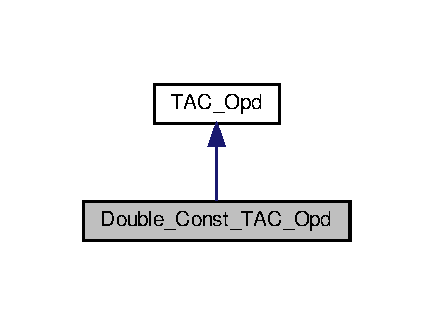
\includegraphics[width=208pt]{classDouble__Const__TAC__Opd__inherit__graph}
\end{center}
\end{figure}


Collaboration diagram for Double\+\_\+\+Const\+\_\+\+T\+A\+C\+\_\+\+Opd\+:
\nopagebreak
\begin{figure}[H]
\begin{center}
\leavevmode
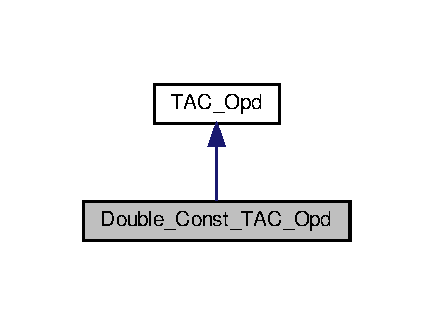
\includegraphics[width=208pt]{classDouble__Const__TAC__Opd__coll__graph}
\end{center}
\end{figure}
\subsection*{Public Member Functions}
\begin{DoxyCompactItemize}
\item 
\mbox{\Hypertarget{classDouble__Const__TAC__Opd_a4b8623ce1c7dcdaecf35352911e9a258}\label{classDouble__Const__TAC__Opd_a4b8623ce1c7dcdaecf35352911e9a258}} 
{\bfseries Double\+\_\+\+Const\+\_\+\+T\+A\+C\+\_\+\+Opd} (double num)
\item 
\mbox{\Hypertarget{classDouble__Const__TAC__Opd_a690703028bf111b13fcd8e3a725c9fad}\label{classDouble__Const__TAC__Opd_a690703028bf111b13fcd8e3a725c9fad}} 
void {\bfseries print\+\_\+opd} (ostream \&file\+\_\+buffer)
\item 
\mbox{\Hypertarget{classDouble__Const__TAC__Opd_a51690fe3e397245f85b372c4fe284d78}\label{classDouble__Const__TAC__Opd_a51690fe3e397245f85b372c4fe284d78}} 
\hyperlink{classRTL__For__TAC}{R\+T\+L\+\_\+\+For\+\_\+\+T\+AC} \& {\bfseries create\+\_\+load\+\_\+stmt} ()
\item 
\mbox{\Hypertarget{classDouble__Const__TAC__Opd_acbfaed86f4baecd629f2ea4d420e9614}\label{classDouble__Const__TAC__Opd_acbfaed86f4baecd629f2ea4d420e9614}} 
Data\+\_\+\+Type {\bfseries get\+\_\+data\+\_\+type} ()
\item 
\mbox{\Hypertarget{classDouble__Const__TAC__Opd_ac0b3bd904d684cc02406dee4ed1df46e}\label{classDouble__Const__TAC__Opd_ac0b3bd904d684cc02406dee4ed1df46e}} 
\hyperlink{classDouble__Const__TAC__Opd}{Double\+\_\+\+Const\+\_\+\+T\+A\+C\+\_\+\+Opd} \& {\bfseries operator=} (const \hyperlink{classDouble__Const__TAC__Opd}{Double\+\_\+\+Const\+\_\+\+T\+A\+C\+\_\+\+Opd} \&rhs)
\end{DoxyCompactItemize}


The documentation for this class was generated from the following files\+:\begin{DoxyCompactItemize}
\item 
tac.\+hh\item 
rtl-\/gen.\+cc\item 
tac.\+cc\end{DoxyCompactItemize}

\hypertarget{classGoto__TAC__Stmt}{}\section{Goto\+\_\+\+T\+A\+C\+\_\+\+Stmt Class Reference}
\label{classGoto__TAC__Stmt}\index{Goto\+\_\+\+T\+A\+C\+\_\+\+Stmt@{Goto\+\_\+\+T\+A\+C\+\_\+\+Stmt}}


Inheritance diagram for Goto\+\_\+\+T\+A\+C\+\_\+\+Stmt\+:
\nopagebreak
\begin{figure}[H]
\begin{center}
\leavevmode
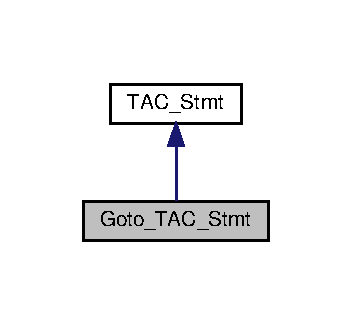
\includegraphics[width=169pt]{classGoto__TAC__Stmt__inherit__graph}
\end{center}
\end{figure}


Collaboration diagram for Goto\+\_\+\+T\+A\+C\+\_\+\+Stmt\+:
\nopagebreak
\begin{figure}[H]
\begin{center}
\leavevmode
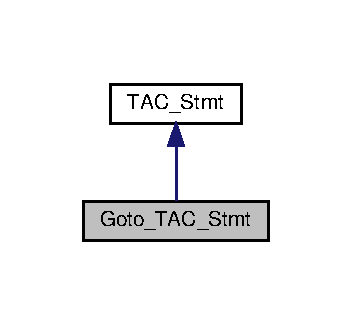
\includegraphics[width=169pt]{classGoto__TAC__Stmt__coll__graph}
\end{center}
\end{figure}
\subsection*{Public Member Functions}
\begin{DoxyCompactItemize}
\item 
\mbox{\Hypertarget{classGoto__TAC__Stmt_a787f210c9dcb0809abdab9c6b7f594cd}\label{classGoto__TAC__Stmt_a787f210c9dcb0809abdab9c6b7f594cd}} 
{\bfseries Goto\+\_\+\+T\+A\+C\+\_\+\+Stmt} (\hyperlink{classTAC__Opd}{T\+A\+C\+\_\+\+Opd} $\ast$result)
\item 
\mbox{\Hypertarget{classGoto__TAC__Stmt_a30332b7ee16239b848174152a0b2d7b3}\label{classGoto__TAC__Stmt_a30332b7ee16239b848174152a0b2d7b3}} 
\hyperlink{classTAC__Opd}{T\+A\+C\+\_\+\+Opd} $\ast$ {\bfseries get\+\_\+result} ()
\item 
\mbox{\Hypertarget{classGoto__TAC__Stmt_a156ec78b2ed1c5b1d1be54213d151354}\label{classGoto__TAC__Stmt_a156ec78b2ed1c5b1d1be54213d151354}} 
void {\bfseries set\+\_\+result} (\hyperlink{classTAC__Opd}{T\+A\+C\+\_\+\+Opd} $\ast$result)
\item 
\mbox{\Hypertarget{classGoto__TAC__Stmt_ae3dff8f35b92af225024d0e0d5f0a455}\label{classGoto__TAC__Stmt_ae3dff8f35b92af225024d0e0d5f0a455}} 
void {\bfseries print\+\_\+tac\+\_\+stmt} (ostream \&file\+\_\+buffer)
\end{DoxyCompactItemize}
\subsection*{Additional Inherited Members}


The documentation for this class was generated from the following files\+:\begin{DoxyCompactItemize}
\item 
tac.\+hh\item 
tac.\+cc\end{DoxyCompactItemize}

\hypertarget{classIf__Goto__TAC__Stmt}{}\section{If\+\_\+\+Goto\+\_\+\+T\+A\+C\+\_\+\+Stmt Class Reference}
\label{classIf__Goto__TAC__Stmt}\index{If\+\_\+\+Goto\+\_\+\+T\+A\+C\+\_\+\+Stmt@{If\+\_\+\+Goto\+\_\+\+T\+A\+C\+\_\+\+Stmt}}


{\ttfamily \#include $<$tac.\+hh$>$}



Inheritance diagram for If\+\_\+\+Goto\+\_\+\+T\+A\+C\+\_\+\+Stmt\+:
\nopagebreak
\begin{figure}[H]
\begin{center}
\leavevmode
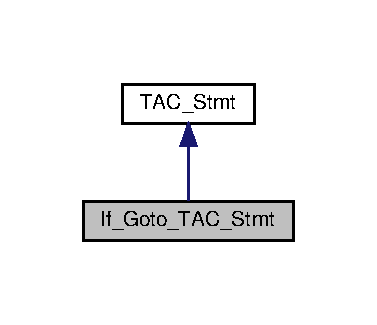
\includegraphics[width=181pt]{classIf__Goto__TAC__Stmt__inherit__graph}
\end{center}
\end{figure}


Collaboration diagram for If\+\_\+\+Goto\+\_\+\+T\+A\+C\+\_\+\+Stmt\+:
\nopagebreak
\begin{figure}[H]
\begin{center}
\leavevmode
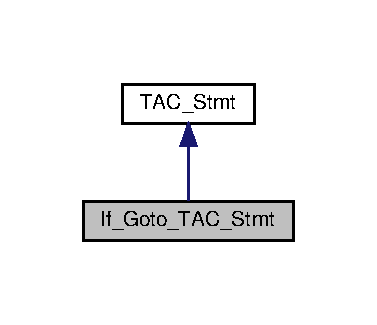
\includegraphics[width=181pt]{classIf__Goto__TAC__Stmt__coll__graph}
\end{center}
\end{figure}
\subsection*{Public Member Functions}
\begin{DoxyCompactItemize}
\item 
\mbox{\Hypertarget{classIf__Goto__TAC__Stmt_ae365b561d6e9b768e58349389909c97c}\label{classIf__Goto__TAC__Stmt_ae365b561d6e9b768e58349389909c97c}} 
{\bfseries If\+\_\+\+Goto\+\_\+\+T\+A\+C\+\_\+\+Stmt} (\hyperlink{classTAC__Opd}{T\+A\+C\+\_\+\+Opd} $\ast$opd1, \hyperlink{classTAC__Opd}{T\+A\+C\+\_\+\+Opd} $\ast$l)
\item 
\mbox{\Hypertarget{classIf__Goto__TAC__Stmt_a9bee36f5c916941da93c02d99ac99ed6}\label{classIf__Goto__TAC__Stmt_a9bee36f5c916941da93c02d99ac99ed6}} 
\hyperlink{classTAC__Opd}{T\+A\+C\+\_\+\+Opd} $\ast$ {\bfseries get\+\_\+opd1} ()
\item 
\mbox{\Hypertarget{classIf__Goto__TAC__Stmt_a4494d0d46cc3400da8cbe172293559a5}\label{classIf__Goto__TAC__Stmt_a4494d0d46cc3400da8cbe172293559a5}} 
\hyperlink{classTAC__Opd}{T\+A\+C\+\_\+\+Opd} $\ast$ {\bfseries get\+\_\+result} ()
\item 
\mbox{\Hypertarget{classIf__Goto__TAC__Stmt_ac8698814cb1f82da52ed5e3549d17359}\label{classIf__Goto__TAC__Stmt_ac8698814cb1f82da52ed5e3549d17359}} 
void {\bfseries set\+\_\+opd1} (\hyperlink{classTAC__Opd}{T\+A\+C\+\_\+\+Opd} $\ast$opd)
\item 
\mbox{\Hypertarget{classIf__Goto__TAC__Stmt_af5eab646c32b38b9b1e3d1b7c302bec7}\label{classIf__Goto__TAC__Stmt_af5eab646c32b38b9b1e3d1b7c302bec7}} 
void {\bfseries set\+\_\+result} (\hyperlink{classTAC__Opd}{T\+A\+C\+\_\+\+Opd} $\ast$result)
\item 
\mbox{\Hypertarget{classIf__Goto__TAC__Stmt_a4d3a5e294299d4a2493bc34775ed317c}\label{classIf__Goto__TAC__Stmt_a4d3a5e294299d4a2493bc34775ed317c}} 
void {\bfseries print\+\_\+tac\+\_\+stmt} (ostream \&file\+\_\+buffer)
\end{DoxyCompactItemize}
\subsection*{Additional Inherited Members}


\subsection{Detailed Description}
T\+AC Control Flow Statement ////////////////////////////// Intraprocedural control flow\+: goto\+\_\+3a, if\+\_\+goto\+\_\+3a, label\+\_\+3a, ////////////////////////////// Interprocedural control flow\+: ret\+\_\+3a, call\+\_\+3a ////////////////////////////// 

The documentation for this class was generated from the following files\+:\begin{DoxyCompactItemize}
\item 
tac.\+hh\item 
tac.\+cc\end{DoxyCompactItemize}

\hypertarget{classInt__Const__Opd}{}\section{Int\+\_\+\+Const\+\_\+\+Opd Class Reference}
\label{classInt__Const__Opd}\index{Int\+\_\+\+Const\+\_\+\+Opd@{Int\+\_\+\+Const\+\_\+\+Opd}}


Inheritance diagram for Int\+\_\+\+Const\+\_\+\+Opd\+:
\nopagebreak
\begin{figure}[H]
\begin{center}
\leavevmode
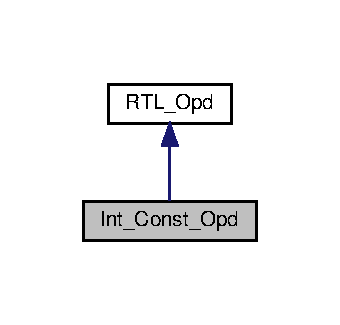
\includegraphics[width=163pt]{classInt__Const__Opd__inherit__graph}
\end{center}
\end{figure}


Collaboration diagram for Int\+\_\+\+Const\+\_\+\+Opd\+:
\nopagebreak
\begin{figure}[H]
\begin{center}
\leavevmode
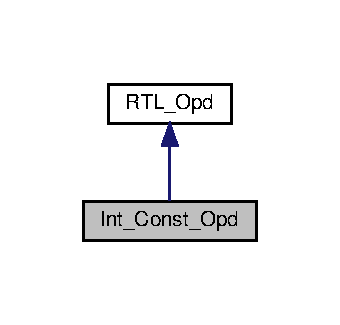
\includegraphics[width=163pt]{classInt__Const__Opd__coll__graph}
\end{center}
\end{figure}
\subsection*{Public Member Functions}
\begin{DoxyCompactItemize}
\item 
\mbox{\Hypertarget{classInt__Const__Opd_ab26b1c8760cbff353bef314e81782d02}\label{classInt__Const__Opd_ab26b1c8760cbff353bef314e81782d02}} 
{\bfseries Int\+\_\+\+Const\+\_\+\+Opd} (int num)
\item 
\mbox{\Hypertarget{classInt__Const__Opd_af407563c29b85b7a42984a02c60d00ce}\label{classInt__Const__Opd_af407563c29b85b7a42984a02c60d00ce}} 
void {\bfseries print\+\_\+rtl\+\_\+opd} (ostream \&file\+\_\+buffer)
\item 
\mbox{\Hypertarget{classInt__Const__Opd_a3ad5d8f89abed16b3ebf5042ac6e3c48}\label{classInt__Const__Opd_a3ad5d8f89abed16b3ebf5042ac6e3c48}} 
void {\bfseries print\+\_\+asm\+\_\+opd} (ostream \&file\+\_\+buffer)
\item 
\mbox{\Hypertarget{classInt__Const__Opd_a3afbfd9248f657304ffdbcd9395e1b4a}\label{classInt__Const__Opd_a3afbfd9248f657304ffdbcd9395e1b4a}} 
\hyperlink{classInt__Const__Opd}{Int\+\_\+\+Const\+\_\+\+Opd} \& {\bfseries operator=} (const \hyperlink{classInt__Const__Opd}{Int\+\_\+\+Const\+\_\+\+Opd} \&rhs)
\end{DoxyCompactItemize}


The documentation for this class was generated from the following files\+:\begin{DoxyCompactItemize}
\item 
rtl.\+hh\item 
rtl.\+cc\end{DoxyCompactItemize}

\hypertarget{classInt__Const__TAC__Opd}{}\section{Int\+\_\+\+Const\+\_\+\+T\+A\+C\+\_\+\+Opd Class Reference}
\label{classInt__Const__TAC__Opd}\index{Int\+\_\+\+Const\+\_\+\+T\+A\+C\+\_\+\+Opd@{Int\+\_\+\+Const\+\_\+\+T\+A\+C\+\_\+\+Opd}}


Inheritance diagram for Int\+\_\+\+Const\+\_\+\+T\+A\+C\+\_\+\+Opd\+:
\nopagebreak
\begin{figure}[H]
\begin{center}
\leavevmode
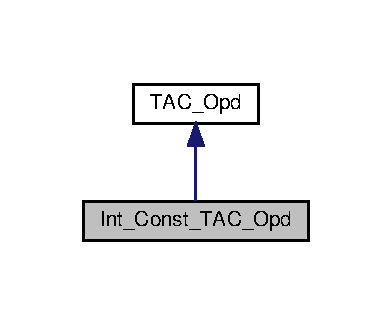
\includegraphics[width=188pt]{classInt__Const__TAC__Opd__inherit__graph}
\end{center}
\end{figure}


Collaboration diagram for Int\+\_\+\+Const\+\_\+\+T\+A\+C\+\_\+\+Opd\+:
\nopagebreak
\begin{figure}[H]
\begin{center}
\leavevmode
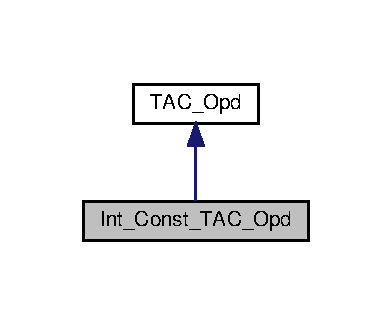
\includegraphics[width=188pt]{classInt__Const__TAC__Opd__coll__graph}
\end{center}
\end{figure}
\subsection*{Public Member Functions}
\begin{DoxyCompactItemize}
\item 
\mbox{\Hypertarget{classInt__Const__TAC__Opd_ab75c34f9d912c61be577c98be1411745}\label{classInt__Const__TAC__Opd_ab75c34f9d912c61be577c98be1411745}} 
{\bfseries Int\+\_\+\+Const\+\_\+\+T\+A\+C\+\_\+\+Opd} (int num)
\item 
\mbox{\Hypertarget{classInt__Const__TAC__Opd_a1ef46bda70c48bf10d422e4b98cecb11}\label{classInt__Const__TAC__Opd_a1ef46bda70c48bf10d422e4b98cecb11}} 
void {\bfseries print\+\_\+opd} (ostream \&file\+\_\+buffer)
\item 
\mbox{\Hypertarget{classInt__Const__TAC__Opd_a89c4d16a0fe5a7f77c0f3ccdc1d035ae}\label{classInt__Const__TAC__Opd_a89c4d16a0fe5a7f77c0f3ccdc1d035ae}} 
\hyperlink{classRTL__For__TAC}{R\+T\+L\+\_\+\+For\+\_\+\+T\+AC} \& {\bfseries create\+\_\+load\+\_\+stmt} ()
\item 
\mbox{\Hypertarget{classInt__Const__TAC__Opd_a9796fb481e155b3fb8cbd2e4fa319598}\label{classInt__Const__TAC__Opd_a9796fb481e155b3fb8cbd2e4fa319598}} 
Data\+\_\+\+Type {\bfseries get\+\_\+data\+\_\+type} ()
\item 
\mbox{\Hypertarget{classInt__Const__TAC__Opd_ae3ab56dfe84d74a24b92c1bb19032bdf}\label{classInt__Const__TAC__Opd_ae3ab56dfe84d74a24b92c1bb19032bdf}} 
\hyperlink{classInt__Const__TAC__Opd}{Int\+\_\+\+Const\+\_\+\+T\+A\+C\+\_\+\+Opd} \& {\bfseries operator=} (const \hyperlink{classInt__Const__TAC__Opd}{Int\+\_\+\+Const\+\_\+\+T\+A\+C\+\_\+\+Opd} \&rhs)
\end{DoxyCompactItemize}


The documentation for this class was generated from the following files\+:\begin{DoxyCompactItemize}
\item 
tac.\+hh\item 
rtl-\/gen.\+cc\item 
tac.\+cc\end{DoxyCompactItemize}

\hypertarget{classIO__TAC__Stmt}{}\section{I\+O\+\_\+\+T\+A\+C\+\_\+\+Stmt Class Reference}
\label{classIO__TAC__Stmt}\index{I\+O\+\_\+\+T\+A\+C\+\_\+\+Stmt@{I\+O\+\_\+\+T\+A\+C\+\_\+\+Stmt}}


Inheritance diagram for I\+O\+\_\+\+T\+A\+C\+\_\+\+Stmt\+:
\nopagebreak
\begin{figure}[H]
\begin{center}
\leavevmode
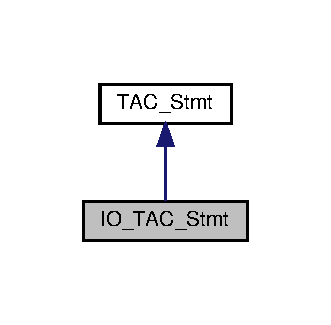
\includegraphics[width=159pt]{classIO__TAC__Stmt__inherit__graph}
\end{center}
\end{figure}


Collaboration diagram for I\+O\+\_\+\+T\+A\+C\+\_\+\+Stmt\+:
\nopagebreak
\begin{figure}[H]
\begin{center}
\leavevmode
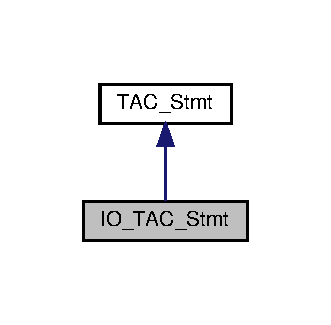
\includegraphics[width=159pt]{classIO__TAC__Stmt__coll__graph}
\end{center}
\end{figure}
\subsection*{Public Member Functions}
\begin{DoxyCompactItemize}
\item 
\mbox{\Hypertarget{classIO__TAC__Stmt_acc16fd7c869edf7a981cafb51b3e7f06}\label{classIO__TAC__Stmt_acc16fd7c869edf7a981cafb51b3e7f06}} 
{\bfseries I\+O\+\_\+\+T\+A\+C\+\_\+\+Stmt} (T\+A\+C\+\_\+\+Op op, \hyperlink{classTAC__Opd}{T\+A\+C\+\_\+\+Opd} $\ast$opd1)
\item 
\mbox{\Hypertarget{classIO__TAC__Stmt_a712acca06971c5af83f3c62b5ff04e86}\label{classIO__TAC__Stmt_a712acca06971c5af83f3c62b5ff04e86}} 
\hyperlink{classTAC__Opd}{T\+A\+C\+\_\+\+Opd} $\ast$ {\bfseries get\+\_\+opd1} ()
\item 
\mbox{\Hypertarget{classIO__TAC__Stmt_a7f925b2cd81b011f70212570f997203d}\label{classIO__TAC__Stmt_a7f925b2cd81b011f70212570f997203d}} 
void {\bfseries set\+\_\+opd1} (\hyperlink{classTAC__Opd}{T\+A\+C\+\_\+\+Opd} $\ast$opd)
\item 
\mbox{\Hypertarget{classIO__TAC__Stmt_a3b7a7551023ee553dd6e6c44b97a102f}\label{classIO__TAC__Stmt_a3b7a7551023ee553dd6e6c44b97a102f}} 
\hyperlink{classRTL__For__TAC}{R\+T\+L\+\_\+\+For\+\_\+\+T\+AC} \& {\bfseries gen\+\_\+rtl} ()
\item 
\mbox{\Hypertarget{classIO__TAC__Stmt_a19c54827b271e333a4b8d5a63d78fe58}\label{classIO__TAC__Stmt_a19c54827b271e333a4b8d5a63d78fe58}} 
void {\bfseries print\+\_\+tac\+\_\+stmt} (ostream \&file\+\_\+buffer)
\end{DoxyCompactItemize}
\subsection*{Additional Inherited Members}


The documentation for this class was generated from the following files\+:\begin{DoxyCompactItemize}
\item 
tac.\+hh\item 
rtl-\/gen.\+cc\item 
tac.\+cc\end{DoxyCompactItemize}

\hypertarget{classIteration__Statement__Ast}{}\section{Iteration\+\_\+\+Statement\+\_\+\+Ast Class Reference}
\label{classIteration__Statement__Ast}\index{Iteration\+\_\+\+Statement\+\_\+\+Ast@{Iteration\+\_\+\+Statement\+\_\+\+Ast}}


Inheritance diagram for Iteration\+\_\+\+Statement\+\_\+\+Ast\+:
\nopagebreak
\begin{figure}[H]
\begin{center}
\leavevmode
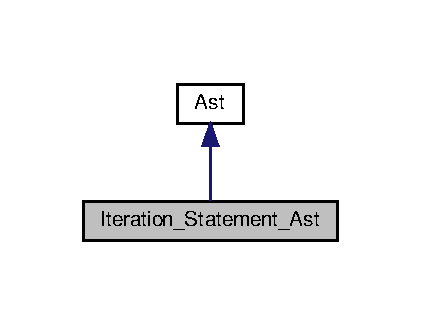
\includegraphics[width=202pt]{classIteration__Statement__Ast__inherit__graph}
\end{center}
\end{figure}


Collaboration diagram for Iteration\+\_\+\+Statement\+\_\+\+Ast\+:
\nopagebreak
\begin{figure}[H]
\begin{center}
\leavevmode
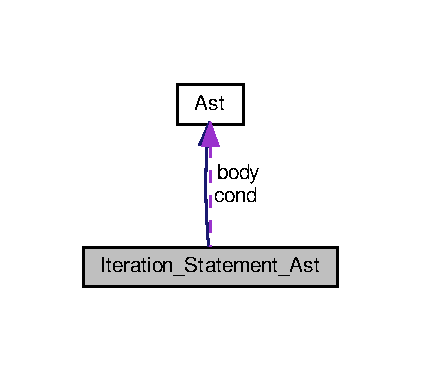
\includegraphics[width=202pt]{classIteration__Statement__Ast__coll__graph}
\end{center}
\end{figure}
\subsection*{Public Member Functions}
\begin{DoxyCompactItemize}
\item 
\mbox{\Hypertarget{classIteration__Statement__Ast_a0c0d47119566eb3d9a19972f652d11c8}\label{classIteration__Statement__Ast_a0c0d47119566eb3d9a19972f652d11c8}} 
{\bfseries Iteration\+\_\+\+Statement\+\_\+\+Ast} (\hyperlink{classAst}{Ast} $\ast$cond, \hyperlink{classAst}{Ast} $\ast$body, int line, bool do\+\_\+form)
\item 
\mbox{\Hypertarget{classIteration__Statement__Ast_a96f25ec81c4786ad487c2b3994c98ad9}\label{classIteration__Statement__Ast_a96f25ec81c4786ad487c2b3994c98ad9}} 
Data\+\_\+\+Type {\bfseries get\+\_\+data\+\_\+type} ()
\item 
\mbox{\Hypertarget{classIteration__Statement__Ast_a04b0649127b06decac624d4cad7e1b9e}\label{classIteration__Statement__Ast_a04b0649127b06decac624d4cad7e1b9e}} 
void {\bfseries set\+\_\+data\+\_\+type} (Data\+\_\+\+Type dt)
\item 
\mbox{\Hypertarget{classIteration__Statement__Ast_a9388f7d8357c08c98e80317150b58f97}\label{classIteration__Statement__Ast_a9388f7d8357c08c98e80317150b58f97}} 
void {\bfseries type\+\_\+check\+\_\+ast} ()
\item 
\mbox{\Hypertarget{classIteration__Statement__Ast_a4aa24a9c9644c5d342280122bdac6bc4}\label{classIteration__Statement__Ast_a4aa24a9c9644c5d342280122bdac6bc4}} 
void {\bfseries print\+\_\+ast} (ostream \&file\+\_\+buffer)
\item 
\mbox{\Hypertarget{classIteration__Statement__Ast_a650fdf53b0e5d7640ae750ed25498dbc}\label{classIteration__Statement__Ast_a650fdf53b0e5d7640ae750ed25498dbc}} 
\hyperlink{classTAC__For__Ast}{T\+A\+C\+\_\+\+For\+\_\+\+Ast} $\ast$ {\bfseries gen\+\_\+tac} ()
\end{DoxyCompactItemize}
\subsection*{Protected Attributes}
\begin{DoxyCompactItemize}
\item 
\mbox{\Hypertarget{classIteration__Statement__Ast_ac95c353c38eb09bbbe786d236f7f5c00}\label{classIteration__Statement__Ast_ac95c353c38eb09bbbe786d236f7f5c00}} 
\hyperlink{classAst}{Ast} $\ast$ {\bfseries cond}
\item 
\mbox{\Hypertarget{classIteration__Statement__Ast_a29ed27e158a5604713c8782de4dad0f8}\label{classIteration__Statement__Ast_a29ed27e158a5604713c8782de4dad0f8}} 
\hyperlink{classAst}{Ast} $\ast$ {\bfseries body}
\item 
\mbox{\Hypertarget{classIteration__Statement__Ast_ac5245b3037441849c8bfc6f670d799b3}\label{classIteration__Statement__Ast_ac5245b3037441849c8bfc6f670d799b3}} 
bool {\bfseries is\+\_\+do\+\_\+form}
\end{DoxyCompactItemize}
\subsection*{Additional Inherited Members}


The documentation for this class was generated from the following files\+:\begin{DoxyCompactItemize}
\item 
ast.\+hh\item 
ast.\+cc\item 
tac-\/gen.\+cc\item 
type-\/checking.\+cc\end{DoxyCompactItemize}

\hypertarget{classLabel__RTL__Stmt}{}\section{Label\+\_\+\+R\+T\+L\+\_\+\+Stmt Class Reference}
\label{classLabel__RTL__Stmt}\index{Label\+\_\+\+R\+T\+L\+\_\+\+Stmt@{Label\+\_\+\+R\+T\+L\+\_\+\+Stmt}}


Inheritance diagram for Label\+\_\+\+R\+T\+L\+\_\+\+Stmt\+:
\nopagebreak
\begin{figure}[H]
\begin{center}
\leavevmode
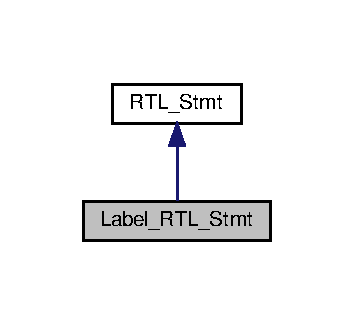
\includegraphics[width=170pt]{classLabel__RTL__Stmt__inherit__graph}
\end{center}
\end{figure}


Collaboration diagram for Label\+\_\+\+R\+T\+L\+\_\+\+Stmt\+:
\nopagebreak
\begin{figure}[H]
\begin{center}
\leavevmode
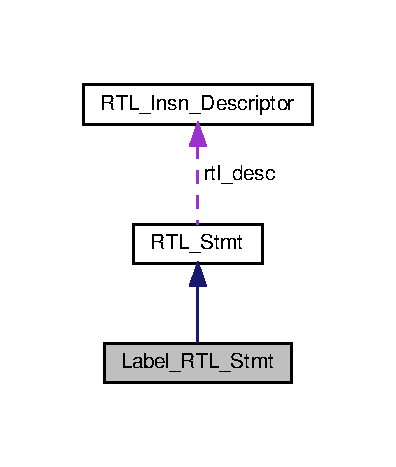
\includegraphics[width=190pt]{classLabel__RTL__Stmt__coll__graph}
\end{center}
\end{figure}
\subsection*{Public Member Functions}
\begin{DoxyCompactItemize}
\item 
\mbox{\Hypertarget{classLabel__RTL__Stmt_a3bb3e6a69c02ef280a7fb1be348d1888}\label{classLabel__RTL__Stmt_a3bb3e6a69c02ef280a7fb1be348d1888}} 
{\bfseries Label\+\_\+\+R\+T\+L\+\_\+\+Stmt} (R\+T\+L\+\_\+\+Op inst\+\_\+op, string label)
\item 
\mbox{\Hypertarget{classLabel__RTL__Stmt_ac83ad285453c7a6d935a9520af63c745}\label{classLabel__RTL__Stmt_ac83ad285453c7a6d935a9520af63c745}} 
\hyperlink{classLabel__RTL__Stmt}{Label\+\_\+\+R\+T\+L\+\_\+\+Stmt} \& {\bfseries operator=} (const \hyperlink{classLabel__RTL__Stmt}{Label\+\_\+\+R\+T\+L\+\_\+\+Stmt} \&rhs)
\item 
\mbox{\Hypertarget{classLabel__RTL__Stmt_ac6cee1f92471f467af10c7b2e53e9b57}\label{classLabel__RTL__Stmt_ac6cee1f92471f467af10c7b2e53e9b57}} 
\hyperlink{classRTL__Insn__Descriptor}{R\+T\+L\+\_\+\+Insn\+\_\+\+Descriptor} \& {\bfseries get\+\_\+inst\+\_\+op\+\_\+of\+\_\+rtl\+\_\+stmt} ()
\item 
\mbox{\Hypertarget{classLabel__RTL__Stmt_a8a9e8c2ac0ee6acbf785bce0e9e705d6}\label{classLabel__RTL__Stmt_a8a9e8c2ac0ee6acbf785bce0e9e705d6}} 
string {\bfseries get\+\_\+label} ()
\item 
\mbox{\Hypertarget{classLabel__RTL__Stmt_a02068853cef52d7410a6b6ef7da68a8f}\label{classLabel__RTL__Stmt_a02068853cef52d7410a6b6ef7da68a8f}} 
void {\bfseries set\+\_\+label} (string label)
\item 
\mbox{\Hypertarget{classLabel__RTL__Stmt_ac000444da441431d5f19bc2ddff2b1ef}\label{classLabel__RTL__Stmt_ac000444da441431d5f19bc2ddff2b1ef}} 
void {\bfseries print\+\_\+rtl\+\_\+stmt} (ostream \&file\+\_\+buffer)
\item 
\mbox{\Hypertarget{classLabel__RTL__Stmt_ad71cba0745bfc084c0078b62ea6bd7bf}\label{classLabel__RTL__Stmt_ad71cba0745bfc084c0078b62ea6bd7bf}} 
void {\bfseries print\+\_\+assembly} (ostream \&file\+\_\+buffer)
\end{DoxyCompactItemize}
\subsection*{Additional Inherited Members}


The documentation for this class was generated from the following files\+:\begin{DoxyCompactItemize}
\item 
rtl.\+hh\item 
rtl.\+cc\end{DoxyCompactItemize}

\hypertarget{classLabel__TAC__Opd}{}\section{Label\+\_\+\+T\+A\+C\+\_\+\+Opd Class Reference}
\label{classLabel__TAC__Opd}\index{Label\+\_\+\+T\+A\+C\+\_\+\+Opd@{Label\+\_\+\+T\+A\+C\+\_\+\+Opd}}


Inheritance diagram for Label\+\_\+\+T\+A\+C\+\_\+\+Opd\+:
\nopagebreak
\begin{figure}[H]
\begin{center}
\leavevmode
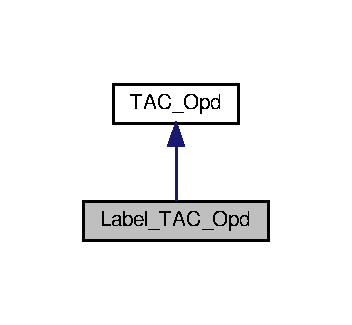
\includegraphics[width=169pt]{classLabel__TAC__Opd__inherit__graph}
\end{center}
\end{figure}


Collaboration diagram for Label\+\_\+\+T\+A\+C\+\_\+\+Opd\+:
\nopagebreak
\begin{figure}[H]
\begin{center}
\leavevmode
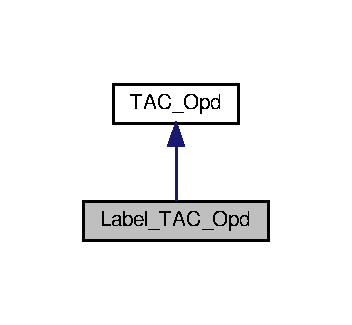
\includegraphics[width=169pt]{classLabel__TAC__Opd__coll__graph}
\end{center}
\end{figure}
\subsection*{Public Member Functions}
\begin{DoxyCompactItemize}
\item 
\mbox{\Hypertarget{classLabel__TAC__Opd_ad7d0d55af1224228a3a1e5b7e0ee8cfc}\label{classLabel__TAC__Opd_ad7d0d55af1224228a3a1e5b7e0ee8cfc}} 
int {\bfseries get\+\_\+label} ()
\item 
\mbox{\Hypertarget{classLabel__TAC__Opd_aef92b743176f4effc7ca8d34941e03e9}\label{classLabel__TAC__Opd_aef92b743176f4effc7ca8d34941e03e9}} 
string {\bfseries get\+\_\+label\+\_\+name} ()
\item 
\mbox{\Hypertarget{classLabel__TAC__Opd_a11242fe9f745c9b6fe9017a1c20541d4}\label{classLabel__TAC__Opd_a11242fe9f745c9b6fe9017a1c20541d4}} 
void {\bfseries print\+\_\+opd} (ostream \&file\+\_\+buffer)
\end{DoxyCompactItemize}


The documentation for this class was generated from the following files\+:\begin{DoxyCompactItemize}
\item 
tac.\+hh\item 
tac.\+cc\end{DoxyCompactItemize}

\hypertarget{classLabel__TAC__Stmt}{}\section{Label\+\_\+\+T\+A\+C\+\_\+\+Stmt Class Reference}
\label{classLabel__TAC__Stmt}\index{Label\+\_\+\+T\+A\+C\+\_\+\+Stmt@{Label\+\_\+\+T\+A\+C\+\_\+\+Stmt}}


Inheritance diagram for Label\+\_\+\+T\+A\+C\+\_\+\+Stmt\+:
\nopagebreak
\begin{figure}[H]
\begin{center}
\leavevmode
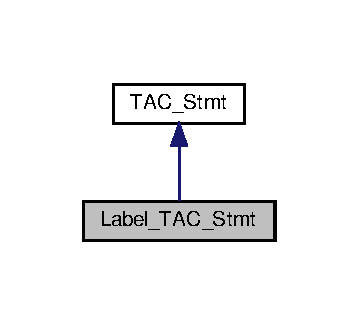
\includegraphics[width=172pt]{classLabel__TAC__Stmt__inherit__graph}
\end{center}
\end{figure}


Collaboration diagram for Label\+\_\+\+T\+A\+C\+\_\+\+Stmt\+:
\nopagebreak
\begin{figure}[H]
\begin{center}
\leavevmode
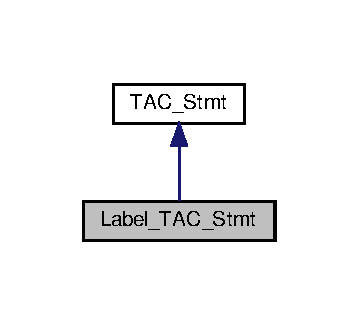
\includegraphics[width=172pt]{classLabel__TAC__Stmt__coll__graph}
\end{center}
\end{figure}
\subsection*{Public Member Functions}
\begin{DoxyCompactItemize}
\item 
\mbox{\Hypertarget{classLabel__TAC__Stmt_a5ed45cdb041cc485db08220057549a68}\label{classLabel__TAC__Stmt_a5ed45cdb041cc485db08220057549a68}} 
{\bfseries Label\+\_\+\+T\+A\+C\+\_\+\+Stmt} (\hyperlink{classTAC__Opd}{T\+A\+C\+\_\+\+Opd} $\ast$label\+\_\+opd)
\item 
\mbox{\Hypertarget{classLabel__TAC__Stmt_a71143ad1a8c25d987feb3456a5439e8c}\label{classLabel__TAC__Stmt_a71143ad1a8c25d987feb3456a5439e8c}} 
int {\bfseries get\+\_\+label} ()
\item 
\mbox{\Hypertarget{classLabel__TAC__Stmt_a7114d5bef231d3471d3b58c13e9f9b82}\label{classLabel__TAC__Stmt_a7114d5bef231d3471d3b58c13e9f9b82}} 
string {\bfseries get\+\_\+label\+\_\+name} ()
\item 
\mbox{\Hypertarget{classLabel__TAC__Stmt_a51cf571c80d963584b832bd30e850033}\label{classLabel__TAC__Stmt_a51cf571c80d963584b832bd30e850033}} 
void {\bfseries print\+\_\+tac\+\_\+stmt} (ostream \&file\+\_\+buffer)
\end{DoxyCompactItemize}
\subsection*{Additional Inherited Members}


The documentation for this class was generated from the following files\+:\begin{DoxyCompactItemize}
\item 
tac.\+hh\item 
tac.\+cc\end{DoxyCompactItemize}

\hypertarget{classLogical__Expr__Ast}{}\section{Logical\+\_\+\+Expr\+\_\+\+Ast Class Reference}
\label{classLogical__Expr__Ast}\index{Logical\+\_\+\+Expr\+\_\+\+Ast@{Logical\+\_\+\+Expr\+\_\+\+Ast}}


Inheritance diagram for Logical\+\_\+\+Expr\+\_\+\+Ast\+:
\nopagebreak
\begin{figure}[H]
\begin{center}
\leavevmode
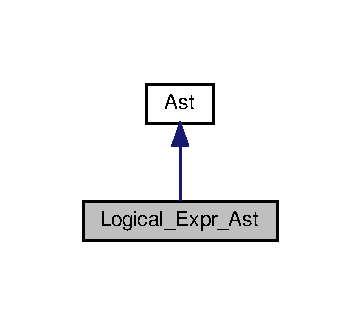
\includegraphics[width=173pt]{classLogical__Expr__Ast__inherit__graph}
\end{center}
\end{figure}


Collaboration diagram for Logical\+\_\+\+Expr\+\_\+\+Ast\+:
\nopagebreak
\begin{figure}[H]
\begin{center}
\leavevmode
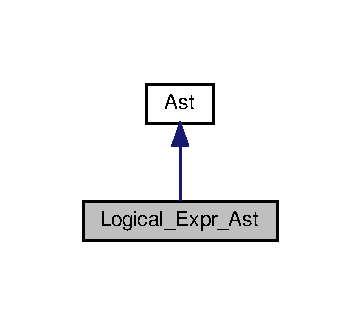
\includegraphics[width=173pt]{classLogical__Expr__Ast__coll__graph}
\end{center}
\end{figure}
\subsection*{Public Member Functions}
\begin{DoxyCompactItemize}
\item 
\mbox{\Hypertarget{classLogical__Expr__Ast_ae83621b708b8c6650cca22edd074c303}\label{classLogical__Expr__Ast_ae83621b708b8c6650cca22edd074c303}} 
{\bfseries Logical\+\_\+\+Expr\+\_\+\+Ast} (\hyperlink{classAst}{Ast} $\ast$lhs, Logical\+\_\+\+Op bop, \hyperlink{classAst}{Ast} $\ast$rhs, int line)
\item 
\mbox{\Hypertarget{classLogical__Expr__Ast_ade9dc17ee7bfe6c416c94e6daf5f2f6b}\label{classLogical__Expr__Ast_ade9dc17ee7bfe6c416c94e6daf5f2f6b}} 
Data\+\_\+\+Type {\bfseries get\+\_\+data\+\_\+type} ()
\item 
\mbox{\Hypertarget{classLogical__Expr__Ast_a8536bd1f73b9d237db6ddd65e5f84878}\label{classLogical__Expr__Ast_a8536bd1f73b9d237db6ddd65e5f84878}} 
void {\bfseries set\+\_\+data\+\_\+type} (Data\+\_\+\+Type dt)
\item 
\mbox{\Hypertarget{classLogical__Expr__Ast_ab361db97f43e08e918a170305d92da9a}\label{classLogical__Expr__Ast_ab361db97f43e08e918a170305d92da9a}} 
void {\bfseries type\+\_\+check\+\_\+ast} ()
\item 
\mbox{\Hypertarget{classLogical__Expr__Ast_aec6696045b9417bbccfc3402261f8c27}\label{classLogical__Expr__Ast_aec6696045b9417bbccfc3402261f8c27}} 
\hyperlink{classTAC__For__Ast}{T\+A\+C\+\_\+\+For\+\_\+\+Ast} $\ast$ {\bfseries gen\+\_\+tac} ()
\item 
\mbox{\Hypertarget{classLogical__Expr__Ast_a280335e08b37cbc2e1b11e16b31407f9}\label{classLogical__Expr__Ast_a280335e08b37cbc2e1b11e16b31407f9}} 
T\+A\+C\+\_\+\+Op {\bfseries get\+\_\+tac\+\_\+operator\+\_\+for\+\_\+logical\+\_\+operator} ()
\item 
\mbox{\Hypertarget{classLogical__Expr__Ast_a68f261c9b9e56fd60fcdb3f0dd634d02}\label{classLogical__Expr__Ast_a68f261c9b9e56fd60fcdb3f0dd634d02}} 
void {\bfseries print\+\_\+ast} (ostream \&file\+\_\+buffer)
\end{DoxyCompactItemize}
\subsection*{Additional Inherited Members}


The documentation for this class was generated from the following files\+:\begin{DoxyCompactItemize}
\item 
ast.\+hh\item 
ast.\+cc\item 
tac-\/gen.\+cc\item 
type-\/checking.\+cc\end{DoxyCompactItemize}

\hypertarget{classMachine__Description}{}\section{Machine\+\_\+\+Description Class Reference}
\label{classMachine__Description}\index{Machine\+\_\+\+Description@{Machine\+\_\+\+Description}}
\subsection*{Public Member Functions}
\begin{DoxyCompactItemize}
\item 
\mbox{\Hypertarget{classMachine__Description_ae41b3d24e739b0f72e2a368e4554d59a}\label{classMachine__Description_ae41b3d24e739b0f72e2a368e4554d59a}} 
void {\bfseries initialize\+\_\+instruction\+\_\+table} ()
\item 
\mbox{\Hypertarget{classMachine__Description_aea2c191e8c23720a89c4c7e1d706fccc}\label{classMachine__Description_aea2c191e8c23720a89c4c7e1d706fccc}} 
void {\bfseries initialize\+\_\+register\+\_\+table} ()
\item 
\mbox{\Hypertarget{classMachine__Description_ac174c5197e269140a1df808528bed17e}\label{classMachine__Description_ac174c5197e269140a1df808528bed17e}} 
void {\bfseries validate\+\_\+init\+\_\+local\+\_\+register\+\_\+mapping\+\_\+before\+\_\+fn\+\_\+call} ()
\item 
\mbox{\Hypertarget{classMachine__Description_a37a985c2f6c5cab5643198fbcfcd612f}\label{classMachine__Description_a37a985c2f6c5cab5643198fbcfcd612f}} 
void {\bfseries validate\+\_\+init\+\_\+local\+\_\+register\+\_\+mapping} ()
\item 
\mbox{\Hypertarget{classMachine__Description_a25249f9cf13799a68d7cb61b4f9f441e}\label{classMachine__Description_a25249f9cf13799a68d7cb61b4f9f441e}} 
void {\bfseries clear\+\_\+local\+\_\+register\+\_\+mappings} ()
\item 
\mbox{\Hypertarget{classMachine__Description_a7e4f6cb207f09ea0af63bbd6d6b4ed0f}\label{classMachine__Description_a7e4f6cb207f09ea0af63bbd6d6b4ed0f}} 
void {\bfseries clear\+\_\+reg\+\_\+not\+\_\+used\+\_\+for\+\_\+expr\+\_\+result} ()
\item 
\mbox{\Hypertarget{classMachine__Description_a48ec0a979193c96cc2358a1734d2a3d2}\label{classMachine__Description_a48ec0a979193c96cc2358a1734d2a3d2}} 
{\footnotesize template$<$Register\+\_\+\+Use\+\_\+\+Category dt$>$ }\\int {\bfseries count\+\_\+free\+\_\+register} ()
\item 
\mbox{\Hypertarget{classMachine__Description_ad87702471660a53e20aecbccc720ee05}\label{classMachine__Description_ad87702471660a53e20aecbccc720ee05}} 
{\footnotesize template$<$Register\+\_\+\+Use\+\_\+\+Category dt$>$ }\\\hyperlink{classRegister__Descriptor}{Register\+\_\+\+Descriptor} $\ast$ {\bfseries get\+\_\+new\+\_\+register} ()
\item 
\mbox{\Hypertarget{classMachine__Description_a2c7d822e878f24f24c81b9797358b4fb}\label{classMachine__Description_a2c7d822e878f24f24c81b9797358b4fb}} 
\hyperlink{classRegister__Descriptor}{Register\+\_\+\+Descriptor} $\ast$ {\bfseries get\+\_\+no\+\_\+reg} ()
\end{DoxyCompactItemize}
\subsection*{Public Attributes}
\begin{DoxyCompactItemize}
\item 
\mbox{\Hypertarget{classMachine__Description_aa122bf738407bb2b3fea850e2cd00fc4}\label{classMachine__Description_aa122bf738407bb2b3fea850e2cd00fc4}} 
map$<$ R\+T\+L\+\_\+\+Op, \hyperlink{classRTL__Insn__Descriptor}{R\+T\+L\+\_\+\+Insn\+\_\+\+Descriptor} $\ast$ $>$ {\bfseries spim\+\_\+instruction\+\_\+table}
\item 
\mbox{\Hypertarget{classMachine__Description_a20b86b8722fdeb33d51055f8a3f81ac9}\label{classMachine__Description_a20b86b8722fdeb33d51055f8a3f81ac9}} 
map$<$ Spim\+\_\+\+Register, \hyperlink{classRegister__Descriptor}{Register\+\_\+\+Descriptor} $\ast$ $>$ {\bfseries spim\+\_\+register\+\_\+table}
\end{DoxyCompactItemize}


The documentation for this class was generated from the following files\+:\begin{DoxyCompactItemize}
\item 
reg-\/alloc.\+hh\item 
reg-\/alloc.\+cc\end{DoxyCompactItemize}

\hypertarget{classMem__Opd}{}\section{Mem\+\_\+\+Opd Class Reference}
\label{classMem__Opd}\index{Mem\+\_\+\+Opd@{Mem\+\_\+\+Opd}}


Inheritance diagram for Mem\+\_\+\+Opd\+:
\nopagebreak
\begin{figure}[H]
\begin{center}
\leavevmode
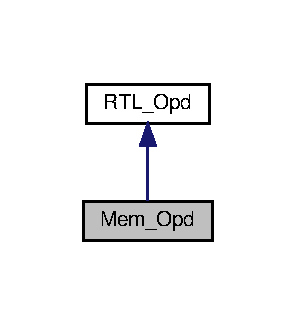
\includegraphics[width=142pt]{classMem__Opd__inherit__graph}
\end{center}
\end{figure}


Collaboration diagram for Mem\+\_\+\+Opd\+:
\nopagebreak
\begin{figure}[H]
\begin{center}
\leavevmode
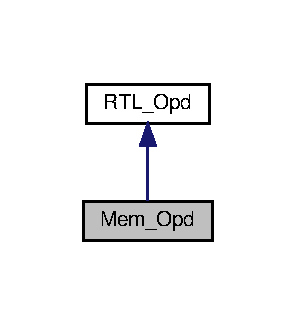
\includegraphics[width=142pt]{classMem__Opd__coll__graph}
\end{center}
\end{figure}
\subsection*{Public Member Functions}
\begin{DoxyCompactItemize}
\item 
\mbox{\Hypertarget{classMem__Opd_aa95863d9f05a550ac54dfe252e8f24b9}\label{classMem__Opd_aa95863d9f05a550ac54dfe252e8f24b9}} 
{\bfseries Mem\+\_\+\+Opd} (\hyperlink{classSymbol__Table__Entry}{Symbol\+\_\+\+Table\+\_\+\+Entry} \&se)
\item 
\mbox{\Hypertarget{classMem__Opd_a47b309bf4b5dfa9067a38f0222eea196}\label{classMem__Opd_a47b309bf4b5dfa9067a38f0222eea196}} 
void {\bfseries print\+\_\+rtl\+\_\+opd} (ostream \&file\+\_\+buffer)
\item 
\mbox{\Hypertarget{classMem__Opd_ac1505a9c24e4538d66984a346473155c}\label{classMem__Opd_ac1505a9c24e4538d66984a346473155c}} 
void {\bfseries print\+\_\+asm\+\_\+opd} (ostream \&file\+\_\+buffer)
\item 
\mbox{\Hypertarget{classMem__Opd_a9579c9d0a10b80807a8703bc82686d9e}\label{classMem__Opd_a9579c9d0a10b80807a8703bc82686d9e}} 
\hyperlink{classMem__Opd}{Mem\+\_\+\+Opd} \& {\bfseries operator=} (const \hyperlink{classMem__Opd}{Mem\+\_\+\+Opd} \&rhs)
\end{DoxyCompactItemize}


The documentation for this class was generated from the following files\+:\begin{DoxyCompactItemize}
\item 
rtl.\+hh\item 
rtl.\+cc\end{DoxyCompactItemize}

\hypertarget{classMinus__Ast}{}\section{Minus\+\_\+\+Ast Class Reference}
\label{classMinus__Ast}\index{Minus\+\_\+\+Ast@{Minus\+\_\+\+Ast}}


Inheritance diagram for Minus\+\_\+\+Ast\+:
\nopagebreak
\begin{figure}[H]
\begin{center}
\leavevmode
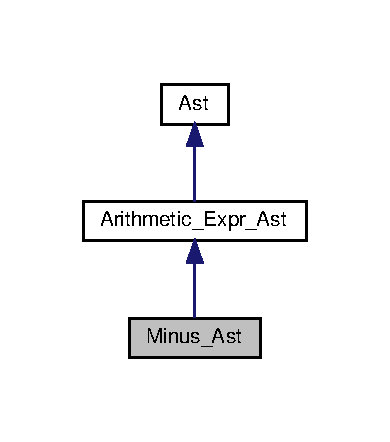
\includegraphics[width=187pt]{classMinus__Ast__inherit__graph}
\end{center}
\end{figure}


Collaboration diagram for Minus\+\_\+\+Ast\+:
\nopagebreak
\begin{figure}[H]
\begin{center}
\leavevmode
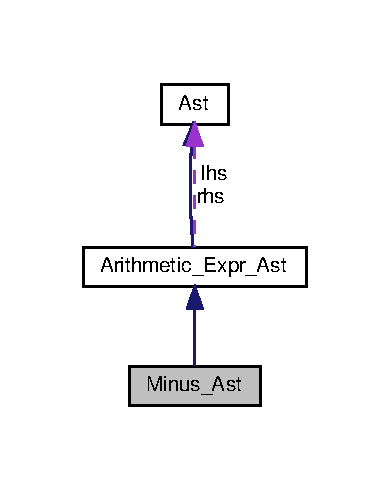
\includegraphics[width=187pt]{classMinus__Ast__coll__graph}
\end{center}
\end{figure}
\subsection*{Public Member Functions}
\begin{DoxyCompactItemize}
\item 
\mbox{\Hypertarget{classMinus__Ast_a98ed432fcc1361417e3c27b88fc87abc}\label{classMinus__Ast_a98ed432fcc1361417e3c27b88fc87abc}} 
{\bfseries Minus\+\_\+\+Ast} (\hyperlink{classAst}{Ast} $\ast$l, \hyperlink{classAst}{Ast} $\ast$r, int line)
\item 
\mbox{\Hypertarget{classMinus__Ast_acda7998d88ecbf15f0efe38ff2258386}\label{classMinus__Ast_acda7998d88ecbf15f0efe38ff2258386}} 
void {\bfseries print\+\_\+ast} (ostream \&file\+\_\+buffer)
\item 
\mbox{\Hypertarget{classMinus__Ast_ad3f07ab3bd23eafd8b3427100ad15c29}\label{classMinus__Ast_ad3f07ab3bd23eafd8b3427100ad15c29}} 
\hyperlink{classTAC__For__Ast}{T\+A\+C\+\_\+\+For\+\_\+\+Ast} $\ast$ {\bfseries gen\+\_\+tac} ()
\end{DoxyCompactItemize}
\subsection*{Additional Inherited Members}


The documentation for this class was generated from the following files\+:\begin{DoxyCompactItemize}
\item 
ast.\+hh\item 
ast.\+cc\item 
tac-\/gen.\+cc\end{DoxyCompactItemize}

\hypertarget{classMove__RTL__Stmt}{}\section{Move\+\_\+\+R\+T\+L\+\_\+\+Stmt Class Reference}
\label{classMove__RTL__Stmt}\index{Move\+\_\+\+R\+T\+L\+\_\+\+Stmt@{Move\+\_\+\+R\+T\+L\+\_\+\+Stmt}}


Inheritance diagram for Move\+\_\+\+R\+T\+L\+\_\+\+Stmt\+:
\nopagebreak
\begin{figure}[H]
\begin{center}
\leavevmode
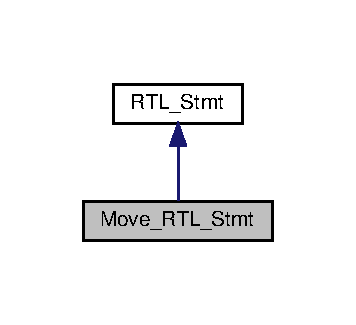
\includegraphics[width=171pt]{classMove__RTL__Stmt__inherit__graph}
\end{center}
\end{figure}


Collaboration diagram for Move\+\_\+\+R\+T\+L\+\_\+\+Stmt\+:
\nopagebreak
\begin{figure}[H]
\begin{center}
\leavevmode
\includegraphics[width=190pt]{classMove__RTL__Stmt__coll__graph}
\end{center}
\end{figure}
\subsection*{Public Member Functions}
\begin{DoxyCompactItemize}
\item 
\mbox{\Hypertarget{classMove__RTL__Stmt_a2563e5ad7f40a37a3287840a3bb0ee9e}\label{classMove__RTL__Stmt_a2563e5ad7f40a37a3287840a3bb0ee9e}} 
{\bfseries Move\+\_\+\+R\+T\+L\+\_\+\+Stmt} (R\+T\+L\+\_\+\+Op inst\+\_\+op, \hyperlink{classRTL__Opd}{R\+T\+L\+\_\+\+Opd} $\ast$opd1, \hyperlink{classRTL__Opd}{R\+T\+L\+\_\+\+Opd} $\ast$result)
\item 
\mbox{\Hypertarget{classMove__RTL__Stmt_ac6b724a936c2d1dee909dc7e6633a368}\label{classMove__RTL__Stmt_ac6b724a936c2d1dee909dc7e6633a368}} 
\hyperlink{classMove__RTL__Stmt}{Move\+\_\+\+R\+T\+L\+\_\+\+Stmt} \& {\bfseries operator=} (const \hyperlink{classMove__RTL__Stmt}{Move\+\_\+\+R\+T\+L\+\_\+\+Stmt} \&rhs)
\item 
\mbox{\Hypertarget{classMove__RTL__Stmt_a7e3d8a1a2e401d29f9500d75f97a32a4}\label{classMove__RTL__Stmt_a7e3d8a1a2e401d29f9500d75f97a32a4}} 
\hyperlink{classRTL__Insn__Descriptor}{R\+T\+L\+\_\+\+Insn\+\_\+\+Descriptor} \& {\bfseries get\+\_\+inst\+\_\+op\+\_\+of\+\_\+rtl\+\_\+stmt} ()
\item 
\mbox{\Hypertarget{classMove__RTL__Stmt_a5e1392d7c9756274a3b3a978c807d66c}\label{classMove__RTL__Stmt_a5e1392d7c9756274a3b3a978c807d66c}} 
\hyperlink{classRTL__Opd}{R\+T\+L\+\_\+\+Opd} $\ast$ {\bfseries get\+\_\+opd1} ()
\item 
\mbox{\Hypertarget{classMove__RTL__Stmt_ab125481e8172caa3c91bfab5966cc2c8}\label{classMove__RTL__Stmt_ab125481e8172caa3c91bfab5966cc2c8}} 
void {\bfseries set\+\_\+opd1} (\hyperlink{classRTL__Opd}{R\+T\+L\+\_\+\+Opd} $\ast$io)
\item 
\mbox{\Hypertarget{classMove__RTL__Stmt_ac30662deb6e903c282985fd1145574d2}\label{classMove__RTL__Stmt_ac30662deb6e903c282985fd1145574d2}} 
\hyperlink{classRTL__Opd}{R\+T\+L\+\_\+\+Opd} $\ast$ {\bfseries get\+\_\+result} ()
\item 
\mbox{\Hypertarget{classMove__RTL__Stmt_a6bac27eb25c7704bb0f330b378df87fd}\label{classMove__RTL__Stmt_a6bac27eb25c7704bb0f330b378df87fd}} 
void {\bfseries set\+\_\+result} (\hyperlink{classRTL__Opd}{R\+T\+L\+\_\+\+Opd} $\ast$io)
\item 
\mbox{\Hypertarget{classMove__RTL__Stmt_a62a25f356a2ee0a9c1121f7d53992a0d}\label{classMove__RTL__Stmt_a62a25f356a2ee0a9c1121f7d53992a0d}} 
void {\bfseries print\+\_\+rtl\+\_\+stmt} (ostream \&file\+\_\+buffer)
\item 
\mbox{\Hypertarget{classMove__RTL__Stmt_af2af8e9e0693c63de001f2682b07813c}\label{classMove__RTL__Stmt_af2af8e9e0693c63de001f2682b07813c}} 
void {\bfseries print\+\_\+assembly} (ostream \&file\+\_\+buffer)
\end{DoxyCompactItemize}
\subsection*{Additional Inherited Members}


The documentation for this class was generated from the following files\+:\begin{DoxyCompactItemize}
\item 
rtl.\+hh\item 
rtl.\+cc\end{DoxyCompactItemize}

\hypertarget{classMult__Ast}{}\section{Mult\+\_\+\+Ast Class Reference}
\label{classMult__Ast}\index{Mult\+\_\+\+Ast@{Mult\+\_\+\+Ast}}


Inheritance diagram for Mult\+\_\+\+Ast\+:
\nopagebreak
\begin{figure}[H]
\begin{center}
\leavevmode
\includegraphics[width=187pt]{classMult__Ast__inherit__graph}
\end{center}
\end{figure}


Collaboration diagram for Mult\+\_\+\+Ast\+:
\nopagebreak
\begin{figure}[H]
\begin{center}
\leavevmode
\includegraphics[width=187pt]{classMult__Ast__coll__graph}
\end{center}
\end{figure}
\subsection*{Public Member Functions}
\begin{DoxyCompactItemize}
\item 
\mbox{\Hypertarget{classMult__Ast_ab2c5f076dc7d34512400b35aaa8069fb}\label{classMult__Ast_ab2c5f076dc7d34512400b35aaa8069fb}} 
{\bfseries Mult\+\_\+\+Ast} (\hyperlink{classAst}{Ast} $\ast$l, \hyperlink{classAst}{Ast} $\ast$r, int line)
\item 
\mbox{\Hypertarget{classMult__Ast_acd7447739711e14d94d1a596ace6f616}\label{classMult__Ast_acd7447739711e14d94d1a596ace6f616}} 
void {\bfseries print\+\_\+ast} (ostream \&file\+\_\+buffer)
\item 
\mbox{\Hypertarget{classMult__Ast_aafbf6a8f992fcdd0948fa23190c27674}\label{classMult__Ast_aafbf6a8f992fcdd0948fa23190c27674}} 
\hyperlink{classTAC__For__Ast}{T\+A\+C\+\_\+\+For\+\_\+\+Ast} $\ast$ {\bfseries gen\+\_\+tac} ()
\end{DoxyCompactItemize}
\subsection*{Additional Inherited Members}


The documentation for this class was generated from the following files\+:\begin{DoxyCompactItemize}
\item 
ast.\+hh\item 
ast.\+cc\item 
tac-\/gen.\+cc\end{DoxyCompactItemize}

\hypertarget{className__Ast}{}\section{Name\+\_\+\+Ast Class Reference}
\label{className__Ast}\index{Name\+\_\+\+Ast@{Name\+\_\+\+Ast}}


Inheritance diagram for Name\+\_\+\+Ast\+:
\nopagebreak
\begin{figure}[H]
\begin{center}
\leavevmode
\includegraphics[width=143pt]{className__Ast__inherit__graph}
\end{center}
\end{figure}


Collaboration diagram for Name\+\_\+\+Ast\+:
\nopagebreak
\begin{figure}[H]
\begin{center}
\leavevmode
\includegraphics[width=143pt]{className__Ast__coll__graph}
\end{center}
\end{figure}
\subsection*{Public Member Functions}
\begin{DoxyCompactItemize}
\item 
\mbox{\Hypertarget{className__Ast_aa73792d7592a8591fe1e3a537010684e}\label{className__Ast_aa73792d7592a8591fe1e3a537010684e}} 
{\bfseries Name\+\_\+\+Ast} (string \&name, \hyperlink{classSymbol__Table__Entry}{Symbol\+\_\+\+Table\+\_\+\+Entry} \&var\+\_\+entry, int line)
\item 
\mbox{\Hypertarget{className__Ast_afe2edab510b3ceddbe40935b32e06a82}\label{className__Ast_afe2edab510b3ceddbe40935b32e06a82}} 
Data\+\_\+\+Type {\bfseries get\+\_\+data\+\_\+type} ()
\item 
\mbox{\Hypertarget{className__Ast_a877fae84cc08c4102287da72162211a7}\label{className__Ast_a877fae84cc08c4102287da72162211a7}} 
\hyperlink{classSymbol__Table__Entry}{Symbol\+\_\+\+Table\+\_\+\+Entry} \& {\bfseries get\+\_\+symbol\+\_\+entry} ()
\item 
\mbox{\Hypertarget{className__Ast_a985865998af4ac911af0a35485d597c0}\label{className__Ast_a985865998af4ac911af0a35485d597c0}} 
void {\bfseries set\+\_\+data\+\_\+type} (Data\+\_\+\+Type dt)
\item 
\mbox{\Hypertarget{className__Ast_a5eb6335143d6d4668cd4068a08732927}\label{className__Ast_a5eb6335143d6d4668cd4068a08732927}} 
void {\bfseries print\+\_\+ast} (ostream \&file\+\_\+buffer)
\item 
\mbox{\Hypertarget{className__Ast_a576275f403384e19f023879ab4ca493b}\label{className__Ast_a576275f403384e19f023879ab4ca493b}} 
\hyperlink{classTAC__For__Ast}{T\+A\+C\+\_\+\+For\+\_\+\+Ast} $\ast$ {\bfseries gen\+\_\+tac} ()
\end{DoxyCompactItemize}
\subsection*{Additional Inherited Members}


The documentation for this class was generated from the following files\+:\begin{DoxyCompactItemize}
\item 
ast.\+hh\item 
ast.\+cc\item 
tac-\/gen.\+cc\end{DoxyCompactItemize}

\hypertarget{classNOP__TAC__Stmt}{}\section{N\+O\+P\+\_\+\+T\+A\+C\+\_\+\+Stmt Class Reference}
\label{classNOP__TAC__Stmt}\index{N\+O\+P\+\_\+\+T\+A\+C\+\_\+\+Stmt@{N\+O\+P\+\_\+\+T\+A\+C\+\_\+\+Stmt}}


Inheritance diagram for N\+O\+P\+\_\+\+T\+A\+C\+\_\+\+Stmt\+:
\nopagebreak
\begin{figure}[H]
\begin{center}
\leavevmode
\includegraphics[width=170pt]{classNOP__TAC__Stmt__inherit__graph}
\end{center}
\end{figure}


Collaboration diagram for N\+O\+P\+\_\+\+T\+A\+C\+\_\+\+Stmt\+:
\nopagebreak
\begin{figure}[H]
\begin{center}
\leavevmode
\includegraphics[width=170pt]{classNOP__TAC__Stmt__coll__graph}
\end{center}
\end{figure}
\subsection*{Public Member Functions}
\begin{DoxyCompactItemize}
\item 
\mbox{\Hypertarget{classNOP__TAC__Stmt_a12941d3f0b384ff5569af91ba5842cb0}\label{classNOP__TAC__Stmt_a12941d3f0b384ff5569af91ba5842cb0}} 
void {\bfseries print\+\_\+tac\+\_\+stmt} (ostream \&file\+\_\+buffer)
\end{DoxyCompactItemize}
\subsection*{Additional Inherited Members}


The documentation for this class was generated from the following file\+:\begin{DoxyCompactItemize}
\item 
tac.\+hh\end{DoxyCompactItemize}

\hypertarget{classNumber__Ast}{}\section{Number\+\_\+\+Ast$<$ T $>$ Class Template Reference}
\label{classNumber__Ast}\index{Number\+\_\+\+Ast$<$ T $>$@{Number\+\_\+\+Ast$<$ T $>$}}


Inheritance diagram for Number\+\_\+\+Ast$<$ T $>$\+:
\nopagebreak
\begin{figure}[H]
\begin{center}
\leavevmode
\includegraphics[width=175pt]{classNumber__Ast__inherit__graph}
\end{center}
\end{figure}


Collaboration diagram for Number\+\_\+\+Ast$<$ T $>$\+:
\nopagebreak
\begin{figure}[H]
\begin{center}
\leavevmode
\includegraphics[width=175pt]{classNumber__Ast__coll__graph}
\end{center}
\end{figure}
\subsection*{Public Member Functions}
\begin{DoxyCompactItemize}
\item 
\mbox{\Hypertarget{classNumber__Ast_a43c07513519b323df1c52c19e6b7a29c}\label{classNumber__Ast_a43c07513519b323df1c52c19e6b7a29c}} 
{\bfseries Number\+\_\+\+Ast} (T number, Data\+\_\+\+Type constant\+\_\+data\+\_\+type, int line)
\item 
\mbox{\Hypertarget{classNumber__Ast_abbab495337bff5e8ae43322a98a5f7a7}\label{classNumber__Ast_abbab495337bff5e8ae43322a98a5f7a7}} 
Data\+\_\+\+Type {\bfseries get\+\_\+data\+\_\+type} ()
\item 
\mbox{\Hypertarget{classNumber__Ast_ae0217e559149200f07ce70e0047d8785}\label{classNumber__Ast_ae0217e559149200f07ce70e0047d8785}} 
void {\bfseries set\+\_\+data\+\_\+type} (Data\+\_\+\+Type dt)
\item 
\mbox{\Hypertarget{classNumber__Ast_a7d4dc495968e66a73a6a894031e3b1cf}\label{classNumber__Ast_a7d4dc495968e66a73a6a894031e3b1cf}} 
bool {\bfseries is\+\_\+value\+\_\+zero} ()
\item 
\mbox{\Hypertarget{classNumber__Ast_a96f8e53ff56d1b047b4f59cef58eb9b6}\label{classNumber__Ast_a96f8e53ff56d1b047b4f59cef58eb9b6}} 
void {\bfseries print\+\_\+ast} (ostream \&file\+\_\+buffer)
\item 
\mbox{\Hypertarget{classNumber__Ast_a9ed2235e0980563bea67140b16c04438}\label{classNumber__Ast_a9ed2235e0980563bea67140b16c04438}} 
\hyperlink{classTAC__For__Ast}{T\+A\+C\+\_\+\+For\+\_\+\+Ast} $\ast$ {\bfseries gen\+\_\+tac} ()
\end{DoxyCompactItemize}
\subsection*{Additional Inherited Members}


The documentation for this class was generated from the following files\+:\begin{DoxyCompactItemize}
\item 
ast.\+hh\item 
ast.\+cc\item 
tac-\/gen.\+cc\end{DoxyCompactItemize}

\hypertarget{classPlus__Ast}{}\section{Plus\+\_\+\+Ast Class Reference}
\label{classPlus__Ast}\index{Plus\+\_\+\+Ast@{Plus\+\_\+\+Ast}}


Inheritance diagram for Plus\+\_\+\+Ast\+:
\nopagebreak
\begin{figure}[H]
\begin{center}
\leavevmode
\includegraphics[width=187pt]{classPlus__Ast__inherit__graph}
\end{center}
\end{figure}


Collaboration diagram for Plus\+\_\+\+Ast\+:
\nopagebreak
\begin{figure}[H]
\begin{center}
\leavevmode
\includegraphics[width=187pt]{classPlus__Ast__coll__graph}
\end{center}
\end{figure}
\subsection*{Public Member Functions}
\begin{DoxyCompactItemize}
\item 
\mbox{\Hypertarget{classPlus__Ast_a436cec2433fe29719c1802fbf634e480}\label{classPlus__Ast_a436cec2433fe29719c1802fbf634e480}} 
{\bfseries Plus\+\_\+\+Ast} (\hyperlink{classAst}{Ast} $\ast$l, \hyperlink{classAst}{Ast} $\ast$r, int line)
\item 
\mbox{\Hypertarget{classPlus__Ast_a476679f8c78244e2025f838a3fbce59f}\label{classPlus__Ast_a476679f8c78244e2025f838a3fbce59f}} 
void {\bfseries print\+\_\+ast} (ostream \&file\+\_\+buffer)
\item 
\mbox{\Hypertarget{classPlus__Ast_ac51762b260d42caa26997ae96a9e204d}\label{classPlus__Ast_ac51762b260d42caa26997ae96a9e204d}} 
\hyperlink{classTAC__For__Ast}{T\+A\+C\+\_\+\+For\+\_\+\+Ast} $\ast$ {\bfseries gen\+\_\+tac} ()
\end{DoxyCompactItemize}
\subsection*{Additional Inherited Members}


The documentation for this class was generated from the following files\+:\begin{DoxyCompactItemize}
\item 
ast.\+hh\item 
ast.\+cc\item 
tac-\/gen.\+cc\end{DoxyCompactItemize}

\hypertarget{classProcedure}{}\section{Procedure Class Reference}
\label{classProcedure}\index{Procedure@{Procedure}}
\subsection*{Public Member Functions}
\begin{DoxyCompactItemize}
\item 
\mbox{\Hypertarget{classProcedure_a79f063eb825cc4653bf1801e01aefcef}\label{classProcedure_a79f063eb825cc4653bf1801e01aefcef}} 
{\bfseries Procedure} (Data\+\_\+\+Type proc\+\_\+return\+\_\+type, string proc\+\_\+name, int line)
\item 
\mbox{\Hypertarget{classProcedure_a9705537b086b1daac7a2ea66d00f39f7}\label{classProcedure_a9705537b086b1daac7a2ea66d00f39f7}} 
void {\bfseries operator==} (\hyperlink{classProcedure}{Procedure} \&proc\+\_\+proto)
\item 
\mbox{\Hypertarget{classProcedure_ad97d178196729055a2e32de026f00e9d}\label{classProcedure_ad97d178196729055a2e32de026f00e9d}} 
void {\bfseries operator=} (\hyperlink{classProcedure}{Procedure} \&proc\+\_\+proto)
\item 
\mbox{\Hypertarget{classProcedure_a0ca44b3ef229d7c426ba83b6f13d3c21}\label{classProcedure_a0ca44b3ef229d7c426ba83b6f13d3c21}} 
bool {\bfseries is\+\_\+proc\+\_\+called} ()
\item 
\mbox{\Hypertarget{classProcedure_ae4f95fa42c39d41583e66fc0fcb4eeee}\label{classProcedure_ae4f95fa42c39d41583e66fc0fcb4eeee}} 
void {\bfseries set\+\_\+proc\+\_\+is\+\_\+called} ()
\item 
\mbox{\Hypertarget{classProcedure_a72476f6329f16a073c359622587664c4}\label{classProcedure_a72476f6329f16a073c359622587664c4}} 
bool {\bfseries is\+\_\+proc\+\_\+defined} ()
\item 
\mbox{\Hypertarget{classProcedure_a1fb033215886edb1461ce6b3dcd22519}\label{classProcedure_a1fb033215886edb1461ce6b3dcd22519}} 
void {\bfseries set\+\_\+proc\+\_\+is\+\_\+defined} ()
\item 
\mbox{\Hypertarget{classProcedure_a12a7f7e39647abf167d3145a8d2f0fee}\label{classProcedure_a12a7f7e39647abf167d3145a8d2f0fee}} 
string {\bfseries get\+\_\+proc\+\_\+name} ()
\item 
\mbox{\Hypertarget{classProcedure_a15f64b0ab32d0a4e8c7a685c24b5b284}\label{classProcedure_a15f64b0ab32d0a4e8c7a685c24b5b284}} 
void {\bfseries set\+\_\+local\+\_\+list} (\hyperlink{classSymbol__Table}{Symbol\+\_\+\+Table} \&new\+\_\+list)
\item 
\mbox{\Hypertarget{classProcedure_abb766661ce9552a111e13fa3c98ab274}\label{classProcedure_abb766661ce9552a111e13fa3c98ab274}} 
\hyperlink{classSymbol__Table}{Symbol\+\_\+\+Table} {\bfseries get\+\_\+local\+\_\+list} ()
\item 
\mbox{\Hypertarget{classProcedure_a75a08cfd0a8401c09d78fec666c87ef3}\label{classProcedure_a75a08cfd0a8401c09d78fec666c87ef3}} 
void {\bfseries set\+\_\+ast\+\_\+list} (list$<$ \hyperlink{classAst}{Ast} $\ast$$>$ \&ast\+\_\+list)
\item 
\mbox{\Hypertarget{classProcedure_a657086c14d842c25c8e20182b1aaac83}\label{classProcedure_a657086c14d842c25c8e20182b1aaac83}} 
void {\bfseries set\+\_\+formal\+\_\+param\+\_\+list} (\hyperlink{classSymbol__Table}{Symbol\+\_\+\+Table} \&new\+\_\+list)
\item 
\mbox{\Hypertarget{classProcedure_a1e102b7cdd97bd7c9097c2f066d0e54e}\label{classProcedure_a1e102b7cdd97bd7c9097c2f066d0e54e}} 
\hyperlink{classSymbol__Table}{Symbol\+\_\+\+Table} \& {\bfseries get\+\_\+formal\+\_\+param\+\_\+list} ()
\item 
\mbox{\Hypertarget{classProcedure_a2d37282048f900e788976e0f836f1b39}\label{classProcedure_a2d37282048f900e788976e0f836f1b39}} 
Data\+\_\+\+Type {\bfseries get\+\_\+return\+\_\+type} ()
\item 
\mbox{\Hypertarget{classProcedure_a53266e4f419e083c1b625936ee5d87a7}\label{classProcedure_a53266e4f419e083c1b625936ee5d87a7}} 
void {\bfseries set\+\_\+return\+\_\+type} (Data\+\_\+\+Type ret\+\_\+type)
\item 
\mbox{\Hypertarget{classProcedure_a27205c6d035b4a1dce8084c1dfb283c8}\label{classProcedure_a27205c6d035b4a1dce8084c1dfb283c8}} 
\hyperlink{classSymbol__Table__Entry}{Symbol\+\_\+\+Table\+\_\+\+Entry} \& {\bfseries get\+\_\+symbol\+\_\+table\+\_\+entry} (string variable\+\_\+name)
\item 
\mbox{\Hypertarget{classProcedure_a9b428954dcaa183d7d9e9de6e9911c59}\label{classProcedure_a9b428954dcaa183d7d9e9de6e9911c59}} 
\hyperlink{classSymbol__Table__Entry}{Symbol\+\_\+\+Table\+\_\+\+Entry} \& {\bfseries get\+\_\+formal\+\_\+param\+\_\+entry} (string variable\+\_\+name)
\item 
\mbox{\Hypertarget{classProcedure_a6c0f80b0f5ee4fab28daa15c7e16d7f0}\label{classProcedure_a6c0f80b0f5ee4fab28daa15c7e16d7f0}} 
void {\bfseries print\+\_\+ast} (ostream \&file\+\_\+buffer)
\item 
\mbox{\Hypertarget{classProcedure_aca7277b92538b9d2ca9934d82bac4d33}\label{classProcedure_aca7277b92538b9d2ca9934d82bac4d33}} 
void {\bfseries print\+\_\+sym} (ostream \&file\+\_\+buffer)
\item 
\mbox{\Hypertarget{classProcedure_a33ef0860b989a8feaef48fdc4f035c96}\label{classProcedure_a33ef0860b989a8feaef48fdc4f035c96}} 
bool {\bfseries variable\+\_\+in\+\_\+symbol\+\_\+list\+\_\+check} (string variable)
\item 
\mbox{\Hypertarget{classProcedure_a6c50be43c82b60709b69a8ad74ad2927}\label{classProcedure_a6c50be43c82b60709b69a8ad74ad2927}} 
bool {\bfseries variable\+\_\+in\+\_\+formal\+\_\+list\+\_\+check} (string variable)
\item 
\mbox{\Hypertarget{classProcedure_ad2a17f54a0cabe054b291705adbe3168}\label{classProcedure_ad2a17f54a0cabe054b291705adbe3168}} 
string {\bfseries get\+\_\+variable\+\_\+in\+\_\+formal\+\_\+list} (int position)
\item 
\mbox{\Hypertarget{classProcedure_af30ac020a911538474d3ad21ed05a01e}\label{classProcedure_af30ac020a911538474d3ad21ed05a01e}} 
void {\bfseries gen\+\_\+tac} ()
\item 
\mbox{\Hypertarget{classProcedure_a31a564b7c85241fb7dcbedfae26deef9}\label{classProcedure_a31a564b7c85241fb7dcbedfae26deef9}} 
void {\bfseries gen\+\_\+rtl} ()
\item 
\mbox{\Hypertarget{classProcedure_a2928b15ac5462dec2c299271659ebd1e}\label{classProcedure_a2928b15ac5462dec2c299271659ebd1e}} 
void {\bfseries print\+\_\+tac} (ostream \&file\+\_\+buffer)
\item 
\mbox{\Hypertarget{classProcedure_ac5033df3107742826a3481fac188906a}\label{classProcedure_ac5033df3107742826a3481fac188906a}} 
void {\bfseries print\+\_\+rtl} (ostream \&file\+\_\+buffer)
\item 
\mbox{\Hypertarget{classProcedure_aa0b4855bad5d9b9de1e159fb9c8a6fdc}\label{classProcedure_aa0b4855bad5d9b9de1e159fb9c8a6fdc}} 
void {\bfseries print\+\_\+assembly} (ostream \&file\+\_\+buffer)
\end{DoxyCompactItemize}


The documentation for this class was generated from the following files\+:\begin{DoxyCompactItemize}
\item 
procedure.\+hh\item 
procedure-\/compile.\+cc\item 
procedure.\+cc\end{DoxyCompactItemize}

\hypertarget{classProgram}{}\section{Program Class Reference}
\label{classProgram}\index{Program@{Program}}
\subsection*{Public Member Functions}
\begin{DoxyCompactItemize}
\item 
\mbox{\Hypertarget{classProgram_ac3f95156b03682c2508523962abcbd18}\label{classProgram_ac3f95156b03682c2508523962abcbd18}} 
void {\bfseries delete\+\_\+all} ()
\item 
\mbox{\Hypertarget{classProgram_adccd7571cec24cf64f22c3ac73a6407e}\label{classProgram_adccd7571cec24cf64f22c3ac73a6407e}} 
\hyperlink{classProcedure}{Procedure} $\ast$ {\bfseries get\+\_\+procedure\+\_\+prototype} (string proc\+\_\+name)
\item 
\mbox{\Hypertarget{classProgram_ac19c7cce514b98bb27c0bc2fafb31645}\label{classProgram_ac19c7cce514b98bb27c0bc2fafb31645}} 
void {\bfseries set\+\_\+proc\+\_\+to\+\_\+map} (string proc\+\_\+name, \hyperlink{classProcedure}{Procedure} $\ast$proc)
\item 
\mbox{\Hypertarget{classProgram_aad148d2a90634f698e006352ceb19fe5}\label{classProgram_aad148d2a90634f698e006352ceb19fe5}} 
void {\bfseries called\+\_\+proc\+\_\+are\+\_\+defined\+\_\+check} ()
\item 
\mbox{\Hypertarget{classProgram_ac0630a98b9fb6198a07ec0044c4a0de7}\label{classProgram_ac0630a98b9fb6198a07ec0044c4a0de7}} 
void {\bfseries set\+\_\+procedure\+\_\+map} (map$<$ string, \hyperlink{classProcedure}{Procedure} $\ast$$>$ \&proc)
\item 
\mbox{\Hypertarget{classProgram_a13156bc0b9bab6b729010ee8572f0f04}\label{classProgram_a13156bc0b9bab6b729010ee8572f0f04}} 
void {\bfseries set\+\_\+procedure} (\hyperlink{classProcedure}{Procedure} $\ast$proc, int line)
\item 
\mbox{\Hypertarget{classProgram_adc447425a4b38f83afc52805b922a021}\label{classProgram_adc447425a4b38f83afc52805b922a021}} 
void {\bfseries set\+\_\+global\+\_\+table} (\hyperlink{classSymbol__Table}{Symbol\+\_\+\+Table} \&new\+\_\+global\+\_\+table)
\item 
\mbox{\Hypertarget{classProgram_ad9c445349520e9782f76200002834f76}\label{classProgram_ad9c445349520e9782f76200002834f76}} 
\hyperlink{classSymbol__Table__Entry}{Symbol\+\_\+\+Table\+\_\+\+Entry} \& {\bfseries get\+\_\+symbol\+\_\+table\+\_\+entry} (string variable)
\item 
\mbox{\Hypertarget{classProgram_ab07994a4f7e065d2e434cb29cb61ffdf}\label{classProgram_ab07994a4f7e065d2e434cb29cb61ffdf}} 
int {\bfseries add\+\_\+string\+\_\+to\+\_\+string\+\_\+table} (string s)
\item 
\mbox{\Hypertarget{classProgram_a62e1a5858c04fa41ca9a0c2eaa20b2c4}\label{classProgram_a62e1a5858c04fa41ca9a0c2eaa20b2c4}} 
string {\bfseries get\+\_\+string} (int str\+\_\+key)
\item 
\mbox{\Hypertarget{classProgram_a6679b78affa93ca6983fc8182b277c41}\label{classProgram_a6679b78affa93ca6983fc8182b277c41}} 
void {\bfseries print\+\_\+sym} ()
\item 
\mbox{\Hypertarget{classProgram_a4eef215eb241fc6b62c70799e1efc7a5}\label{classProgram_a4eef215eb241fc6b62c70799e1efc7a5}} 
void {\bfseries print\+\_\+ast} ()
\item 
\mbox{\Hypertarget{classProgram_a72d775e0b55274f48db4d75130ad32af}\label{classProgram_a72d775e0b55274f48db4d75130ad32af}} 
\hyperlink{classProcedure}{Procedure} $\ast$ {\bfseries get\+\_\+main\+\_\+procedure} (ostream \&file\+\_\+buffer)
\item 
\mbox{\Hypertarget{classProgram_ab0d30db75d63c623d067002b8c4befcd}\label{classProgram_ab0d30db75d63c623d067002b8c4befcd}} 
bool {\bfseries variable\+\_\+proc\+\_\+name\+\_\+check} (string symbol)
\item 
\mbox{\Hypertarget{classProgram_a66d425effdc3a3f26726385e58523c91}\label{classProgram_a66d425effdc3a3f26726385e58523c91}} 
bool {\bfseries variable\+\_\+in\+\_\+symbol\+\_\+list\+\_\+check} (string variable)
\item 
\mbox{\Hypertarget{classProgram_a629ae590baecfa9c8cd85d16290a90ea}\label{classProgram_a629ae590baecfa9c8cd85d16290a90ea}} 
void {\bfseries global\+\_\+list\+\_\+in\+\_\+proc\+\_\+check} ()
\item 
\mbox{\Hypertarget{classProgram_a20b87bdabc4748ee216d3cc18ca9fb24}\label{classProgram_a20b87bdabc4748ee216d3cc18ca9fb24}} 
bool {\bfseries variable\+\_\+in\+\_\+proc\+\_\+map\+\_\+check} (string symbol)
\item 
\mbox{\Hypertarget{classProgram_a5aada4a73fb44c56743499d0cebc7299}\label{classProgram_a5aada4a73fb44c56743499d0cebc7299}} 
void {\bfseries global\+\_\+list\+\_\+in\+\_\+proc\+\_\+map\+\_\+check} ()
\item 
\mbox{\Hypertarget{classProgram_a8cef49bb8efafd1211b545e4a1d1124c}\label{classProgram_a8cef49bb8efafd1211b545e4a1d1124c}} 
bool {\bfseries proc\+\_\+exists} (string proc\+\_\+name)
\item 
\mbox{\Hypertarget{classProgram_a475fd2320538f8e597bb9d849d0405f7}\label{classProgram_a475fd2320538f8e597bb9d849d0405f7}} 
void {\bfseries gen\+\_\+tac} ()
\item 
\mbox{\Hypertarget{classProgram_a45c8d1320b806c2bdbb57fc3aa42074b}\label{classProgram_a45c8d1320b806c2bdbb57fc3aa42074b}} 
void {\bfseries print\+\_\+tac} ()
\item 
\mbox{\Hypertarget{classProgram_a5da38344307cd6b9e50759eec49cb37e}\label{classProgram_a5da38344307cd6b9e50759eec49cb37e}} 
void {\bfseries gen\+\_\+rtl} ()
\item 
\mbox{\Hypertarget{classProgram_a482574e8722887856aa0f11d10bffe99}\label{classProgram_a482574e8722887856aa0f11d10bffe99}} 
void {\bfseries print\+\_\+rtl} ()
\item 
\mbox{\Hypertarget{classProgram_aebdee93c2ea17e9c2a64a72782244f5b}\label{classProgram_aebdee93c2ea17e9c2a64a72782244f5b}} 
void {\bfseries print\+\_\+assembly} ()
\item 
\mbox{\Hypertarget{classProgram_ad3d51e1f71725720471858c8c077cf1b}\label{classProgram_ad3d51e1f71725720471858c8c077cf1b}} 
void {\bfseries print\+\_\+string\+\_\+table} (ostream \&file\+\_\+buffer)
\end{DoxyCompactItemize}


The documentation for this class was generated from the following files\+:\begin{DoxyCompactItemize}
\item 
program.\+hh\item 
program-\/compile.\+cc\item 
program.\+cc\end{DoxyCompactItemize}

\hypertarget{classRead__Ast}{}\section{Read\+\_\+\+Ast Class Reference}
\label{classRead__Ast}\index{Read\+\_\+\+Ast@{Read\+\_\+\+Ast}}


Inheritance diagram for Read\+\_\+\+Ast\+:
\nopagebreak
\begin{figure}[H]
\begin{center}
\leavevmode
\includegraphics[width=140pt]{classRead__Ast__inherit__graph}
\end{center}
\end{figure}


Collaboration diagram for Read\+\_\+\+Ast\+:
\nopagebreak
\begin{figure}[H]
\begin{center}
\leavevmode
\includegraphics[width=140pt]{classRead__Ast__coll__graph}
\end{center}
\end{figure}
\subsection*{Public Member Functions}
\begin{DoxyCompactItemize}
\item 
\mbox{\Hypertarget{classRead__Ast_a41cfed04bdc621bdff39bfd134f0c00e}\label{classRead__Ast_a41cfed04bdc621bdff39bfd134f0c00e}} 
{\bfseries Read\+\_\+\+Ast} (\hyperlink{classAst}{Ast} $\ast$v, int line)
\item 
\mbox{\Hypertarget{classRead__Ast_a17149245f87884aba7bae0c518779e27}\label{classRead__Ast_a17149245f87884aba7bae0c518779e27}} 
void {\bfseries print\+\_\+ast} (ostream \&file\+\_\+buffer)
\item 
\mbox{\Hypertarget{classRead__Ast_a1471603ed7482c7ad518637e200e5ff4}\label{classRead__Ast_a1471603ed7482c7ad518637e200e5ff4}} 
\hyperlink{classTAC__For__Ast}{T\+A\+C\+\_\+\+For\+\_\+\+Ast} $\ast$ {\bfseries gen\+\_\+tac} ()
\end{DoxyCompactItemize}
\subsection*{Additional Inherited Members}


The documentation for this class was generated from the following files\+:\begin{DoxyCompactItemize}
\item 
ast.\+hh\item 
ast.\+cc\item 
tac-\/gen.\+cc\end{DoxyCompactItemize}

\hypertarget{classRead__RTL__Stmt}{}\section{Read\+\_\+\+R\+T\+L\+\_\+\+Stmt Class Reference}
\label{classRead__RTL__Stmt}\index{Read\+\_\+\+R\+T\+L\+\_\+\+Stmt@{Read\+\_\+\+R\+T\+L\+\_\+\+Stmt}}


Inheritance diagram for Read\+\_\+\+R\+T\+L\+\_\+\+Stmt\+:
\nopagebreak
\begin{figure}[H]
\begin{center}
\leavevmode
\includegraphics[width=170pt]{classRead__RTL__Stmt__inherit__graph}
\end{center}
\end{figure}


Collaboration diagram for Read\+\_\+\+R\+T\+L\+\_\+\+Stmt\+:
\nopagebreak
\begin{figure}[H]
\begin{center}
\leavevmode
\includegraphics[width=190pt]{classRead__RTL__Stmt__coll__graph}
\end{center}
\end{figure}
\subsection*{Public Member Functions}
\begin{DoxyCompactItemize}
\item 
\mbox{\Hypertarget{classRead__RTL__Stmt_a02d855d4e53e8fc7afab748677bd7de0}\label{classRead__RTL__Stmt_a02d855d4e53e8fc7afab748677bd7de0}} 
void {\bfseries print\+\_\+rtl\+\_\+stmt} (ostream \&file\+\_\+buffer)
\item 
\mbox{\Hypertarget{classRead__RTL__Stmt_a1c144c83143e468d955dc0e88af01e28}\label{classRead__RTL__Stmt_a1c144c83143e468d955dc0e88af01e28}} 
void {\bfseries print\+\_\+assembly} (ostream \&file\+\_\+buffer)
\end{DoxyCompactItemize}
\subsection*{Additional Inherited Members}


The documentation for this class was generated from the following files\+:\begin{DoxyCompactItemize}
\item 
rtl.\+hh\item 
rtl.\+cc\end{DoxyCompactItemize}

\hypertarget{classRegister__Descriptor}{}\section{Register\+\_\+\+Descriptor Class Reference}
\label{classRegister__Descriptor}\index{Register\+\_\+\+Descriptor@{Register\+\_\+\+Descriptor}}
\subsection*{Public Member Functions}
\begin{DoxyCompactItemize}
\item 
\mbox{\Hypertarget{classRegister__Descriptor_a4aa35608780cc1d3d8788f16c6eafb9f}\label{classRegister__Descriptor_a4aa35608780cc1d3d8788f16c6eafb9f}} 
{\bfseries Register\+\_\+\+Descriptor} (Spim\+\_\+\+Register reg, string nam, Register\+\_\+\+Val\+\_\+\+Type vt, Register\+\_\+\+Use\+\_\+\+Category uc)
\item 
\mbox{\Hypertarget{classRegister__Descriptor_a1d54b888a582927ebcaeba0347c90d72}\label{classRegister__Descriptor_a1d54b888a582927ebcaeba0347c90d72}} 
void {\bfseries update\+\_\+symbol\+\_\+information} (\hyperlink{classSymbol__Table__Entry}{Symbol\+\_\+\+Table\+\_\+\+Entry} \&symbol\+\_\+entry)
\item 
\mbox{\Hypertarget{classRegister__Descriptor_ae32d130d6454fa314bdeca5e2d3106e8}\label{classRegister__Descriptor_ae32d130d6454fa314bdeca5e2d3106e8}} 
bool {\bfseries find\+\_\+symbol\+\_\+entry\+\_\+in\+\_\+list} (\hyperlink{classSymbol__Table__Entry}{Symbol\+\_\+\+Table\+\_\+\+Entry} \&symbol\+\_\+entry)
\item 
\mbox{\Hypertarget{classRegister__Descriptor_a8109c85cdde8d1ec651e7079e426c83c}\label{classRegister__Descriptor_a8109c85cdde8d1ec651e7079e426c83c}} 
void {\bfseries remove\+\_\+symbol\+\_\+entry\+\_\+from\+\_\+list} (\hyperlink{classSymbol__Table__Entry}{Symbol\+\_\+\+Table\+\_\+\+Entry} \&symbol\+\_\+entry)
\item 
\mbox{\Hypertarget{classRegister__Descriptor_a766b921e7c4526dede50426c53e9ea12}\label{classRegister__Descriptor_a766b921e7c4526dede50426c53e9ea12}} 
Register\+\_\+\+Use\+\_\+\+Category {\bfseries get\+\_\+use\+\_\+category} ()
\item 
\mbox{\Hypertarget{classRegister__Descriptor_abf09227ce7ac7523f3868e0d48c80f6b}\label{classRegister__Descriptor_abf09227ce7ac7523f3868e0d48c80f6b}} 
Spim\+\_\+\+Register {\bfseries get\+\_\+register} ()
\item 
\mbox{\Hypertarget{classRegister__Descriptor_a06678f17e2d3bea3e453eaac03bd7af7}\label{classRegister__Descriptor_a06678f17e2d3bea3e453eaac03bd7af7}} 
string {\bfseries get\+\_\+name} ()
\item 
\mbox{\Hypertarget{classRegister__Descriptor_a54997357bf8f247eeb658a01233e78e3}\label{classRegister__Descriptor_a54997357bf8f247eeb658a01233e78e3}} 
Register\+\_\+\+Val\+\_\+\+Type {\bfseries get\+\_\+register\+\_\+type} ()
\item 
\mbox{\Hypertarget{classRegister__Descriptor_ae3d5292f7f3967ca46df5ab410f832e4}\label{classRegister__Descriptor_ae3d5292f7f3967ca46df5ab410f832e4}} 
bool {\bfseries is\+\_\+register\+\_\+occupied} ()
\item 
\mbox{\Hypertarget{classRegister__Descriptor_a9ff043de26a94f43f7e918c98353ee05}\label{classRegister__Descriptor_a9ff043de26a94f43f7e918c98353ee05}} 
void {\bfseries set\+\_\+register\+\_\+occupied} ()
\item 
\mbox{\Hypertarget{classRegister__Descriptor_a5157f9bf84d0bac66fd27b9acf787f90}\label{classRegister__Descriptor_a5157f9bf84d0bac66fd27b9acf787f90}} 
void {\bfseries reset\+\_\+register\+\_\+occupied} ()
\item 
\mbox{\Hypertarget{classRegister__Descriptor_a7488a3ce939e1f98fe7ee26ceef1fef2}\label{classRegister__Descriptor_a7488a3ce939e1f98fe7ee26ceef1fef2}} 
bool {\bfseries is\+\_\+used\+\_\+for\+\_\+fn\+\_\+return} ()
\item 
\mbox{\Hypertarget{classRegister__Descriptor_a030595292125f854b9182f360329773e}\label{classRegister__Descriptor_a030595292125f854b9182f360329773e}} 
void {\bfseries set\+\_\+used\+\_\+for\+\_\+fn\+\_\+return} ()
\item 
\mbox{\Hypertarget{classRegister__Descriptor_a43a472069861c4a32c550b612401446c}\label{classRegister__Descriptor_a43a472069861c4a32c550b612401446c}} 
void {\bfseries reset\+\_\+used\+\_\+for\+\_\+fn\+\_\+return} ()
\item 
\mbox{\Hypertarget{classRegister__Descriptor_a41facbf33871f0c660e2d4db7bc34720}\label{classRegister__Descriptor_a41facbf33871f0c660e2d4db7bc34720}} 
bool {\bfseries is\+\_\+used\+\_\+for\+\_\+expr\+\_\+result} ()
\item 
\mbox{\Hypertarget{classRegister__Descriptor_a0ad91317772df4d41de2748905f3e4b2}\label{classRegister__Descriptor_a0ad91317772df4d41de2748905f3e4b2}} 
void {\bfseries set\+\_\+use\+\_\+for\+\_\+expr\+\_\+result} ()
\item 
\mbox{\Hypertarget{classRegister__Descriptor_a684b04a3a0ea668d4a1186713007b4ed}\label{classRegister__Descriptor_a684b04a3a0ea668d4a1186713007b4ed}} 
void {\bfseries reset\+\_\+use\+\_\+for\+\_\+expr\+\_\+result} ()
\item 
\mbox{\Hypertarget{classRegister__Descriptor_a97126ce0add3175c828489c6f3539849}\label{classRegister__Descriptor_a97126ce0add3175c828489c6f3539849}} 
{\footnotesize template$<$Register\+\_\+\+Use\+\_\+\+Category dt$>$ }\\bool {\bfseries is\+\_\+free} ()
\end{DoxyCompactItemize}


The documentation for this class was generated from the following files\+:\begin{DoxyCompactItemize}
\item 
reg-\/alloc.\+hh\item 
reg-\/alloc.\+cc\end{DoxyCompactItemize}

\hypertarget{classRegister__Opd}{}\section{Register\+\_\+\+Opd Class Reference}
\label{classRegister__Opd}\index{Register\+\_\+\+Opd@{Register\+\_\+\+Opd}}


Inheritance diagram for Register\+\_\+\+Opd\+:
\nopagebreak
\begin{figure}[H]
\begin{center}
\leavevmode
\includegraphics[width=157pt]{classRegister__Opd__inherit__graph}
\end{center}
\end{figure}


Collaboration diagram for Register\+\_\+\+Opd\+:
\nopagebreak
\begin{figure}[H]
\begin{center}
\leavevmode
\includegraphics[width=157pt]{classRegister__Opd__coll__graph}
\end{center}
\end{figure}
\subsection*{Public Member Functions}
\begin{DoxyCompactItemize}
\item 
\mbox{\Hypertarget{classRegister__Opd_ad2ece6a529a3d99a430aec7115b088c2}\label{classRegister__Opd_ad2ece6a529a3d99a430aec7115b088c2}} 
{\bfseries Register\+\_\+\+Opd} (\hyperlink{classRegister__Descriptor}{Register\+\_\+\+Descriptor} $\ast$rd)
\item 
\mbox{\Hypertarget{classRegister__Opd_af946a7d2ed452bac6799305301e4dc75}\label{classRegister__Opd_af946a7d2ed452bac6799305301e4dc75}} 
\hyperlink{classRegister__Descriptor}{Register\+\_\+\+Descriptor} $\ast$ {\bfseries get\+\_\+reg} ()
\item 
\mbox{\Hypertarget{classRegister__Opd_ac909524fc9f8fa2039a0b132c14351b4}\label{classRegister__Opd_ac909524fc9f8fa2039a0b132c14351b4}} 
void {\bfseries print\+\_\+rtl\+\_\+opd} (ostream \&file\+\_\+buffer)
\item 
\mbox{\Hypertarget{classRegister__Opd_ab45b70ad1f1b939665627f7eb633c00c}\label{classRegister__Opd_ab45b70ad1f1b939665627f7eb633c00c}} 
void {\bfseries print\+\_\+asm\+\_\+opd} (ostream \&file\+\_\+buffer)
\item 
\mbox{\Hypertarget{classRegister__Opd_a2870cb4e861064eabbd15c909938c2e4}\label{classRegister__Opd_a2870cb4e861064eabbd15c909938c2e4}} 
\hyperlink{classRegister__Opd}{Register\+\_\+\+Opd} \& {\bfseries operator=} (const \hyperlink{classRegister__Opd}{Register\+\_\+\+Opd} \&rhs)
\end{DoxyCompactItemize}


The documentation for this class was generated from the following files\+:\begin{DoxyCompactItemize}
\item 
rtl.\+hh\item 
rtl.\+cc\end{DoxyCompactItemize}

\hypertarget{classRelational__Expr__Ast}{}\section{Relational\+\_\+\+Expr\+\_\+\+Ast Class Reference}
\label{classRelational__Expr__Ast}\index{Relational\+\_\+\+Expr\+\_\+\+Ast@{Relational\+\_\+\+Expr\+\_\+\+Ast}}


Inheritance diagram for Relational\+\_\+\+Expr\+\_\+\+Ast\+:
\nopagebreak
\begin{figure}[H]
\begin{center}
\leavevmode
\includegraphics[width=186pt]{classRelational__Expr__Ast__inherit__graph}
\end{center}
\end{figure}


Collaboration diagram for Relational\+\_\+\+Expr\+\_\+\+Ast\+:
\nopagebreak
\begin{figure}[H]
\begin{center}
\leavevmode
\includegraphics[width=186pt]{classRelational__Expr__Ast__coll__graph}
\end{center}
\end{figure}
\subsection*{Public Member Functions}
\begin{DoxyCompactItemize}
\item 
\mbox{\Hypertarget{classRelational__Expr__Ast_ad28ee128820b558845b7d14545bcd53f}\label{classRelational__Expr__Ast_ad28ee128820b558845b7d14545bcd53f}} 
{\bfseries Relational\+\_\+\+Expr\+\_\+\+Ast} (\hyperlink{classAst}{Ast} $\ast$lhs, Relational\+\_\+\+Op rop, \hyperlink{classAst}{Ast} $\ast$rhs, int line)
\item 
\mbox{\Hypertarget{classRelational__Expr__Ast_ad266e8a73c627dad1e377978642b89f9}\label{classRelational__Expr__Ast_ad266e8a73c627dad1e377978642b89f9}} 
Data\+\_\+\+Type {\bfseries get\+\_\+data\+\_\+type} ()
\item 
\mbox{\Hypertarget{classRelational__Expr__Ast_a39a7103a6502104eb3f1b783745ac906}\label{classRelational__Expr__Ast_a39a7103a6502104eb3f1b783745ac906}} 
void {\bfseries set\+\_\+data\+\_\+type} (Data\+\_\+\+Type dt)
\item 
\mbox{\Hypertarget{classRelational__Expr__Ast_ae51bc5c519c0dae61628ddaa1396e28f}\label{classRelational__Expr__Ast_ae51bc5c519c0dae61628ddaa1396e28f}} 
void {\bfseries type\+\_\+check\+\_\+ast} ()
\item 
\mbox{\Hypertarget{classRelational__Expr__Ast_a012496a06535337b3fc3c4c6a5c6ee41}\label{classRelational__Expr__Ast_a012496a06535337b3fc3c4c6a5c6ee41}} 
\hyperlink{classTAC__For__Ast}{T\+A\+C\+\_\+\+For\+\_\+\+Ast} $\ast$ {\bfseries gen\+\_\+tac} ()
\item 
\mbox{\Hypertarget{classRelational__Expr__Ast_a37d47c26478e269b2feb97bf59251ffb}\label{classRelational__Expr__Ast_a37d47c26478e269b2feb97bf59251ffb}} 
T\+A\+C\+\_\+\+Op {\bfseries get\+\_\+tac\+\_\+operator\+\_\+for\+\_\+rel\+\_\+operator} ()
\item 
\mbox{\Hypertarget{classRelational__Expr__Ast_aa618711f9c7cd08352da53129d65d9c4}\label{classRelational__Expr__Ast_aa618711f9c7cd08352da53129d65d9c4}} 
void {\bfseries print\+\_\+ast} (ostream \&file\+\_\+buffer)
\end{DoxyCompactItemize}
\subsection*{Additional Inherited Members}


The documentation for this class was generated from the following files\+:\begin{DoxyCompactItemize}
\item 
ast.\+hh\item 
ast.\+cc\item 
tac-\/gen.\+cc\item 
type-\/checking.\+cc\end{DoxyCompactItemize}

\hypertarget{classReturn__Ast}{}\section{Return\+\_\+\+Ast Class Reference}
\label{classReturn__Ast}\index{Return\+\_\+\+Ast@{Return\+\_\+\+Ast}}


Inheritance diagram for Return\+\_\+\+Ast\+:
\nopagebreak
\begin{figure}[H]
\begin{center}
\leavevmode
\includegraphics[width=146pt]{classReturn__Ast__inherit__graph}
\end{center}
\end{figure}


Collaboration diagram for Return\+\_\+\+Ast\+:
\nopagebreak
\begin{figure}[H]
\begin{center}
\leavevmode
\includegraphics[width=146pt]{classReturn__Ast__coll__graph}
\end{center}
\end{figure}
\subsection*{Public Member Functions}
\begin{DoxyCompactItemize}
\item 
\mbox{\Hypertarget{classReturn__Ast_ab02aa131280d8314f894b7d87d443e64}\label{classReturn__Ast_ab02aa131280d8314f894b7d87d443e64}} 
{\bfseries Return\+\_\+\+Ast} (\hyperlink{classAst}{Ast} $\ast$ret\+\_\+val, string name, int line)
\item 
\mbox{\Hypertarget{classReturn__Ast_a26280c96f04206a8690637e35438cf50}\label{classReturn__Ast_a26280c96f04206a8690637e35438cf50}} 
Data\+\_\+\+Type {\bfseries get\+\_\+data\+\_\+type} ()
\item 
\mbox{\Hypertarget{classReturn__Ast_a7861d8777e5ec2d29236fa0402f90a46}\label{classReturn__Ast_a7861d8777e5ec2d29236fa0402f90a46}} 
void {\bfseries print\+\_\+ast} (ostream \&file\+\_\+buffer)
\end{DoxyCompactItemize}
\subsection*{Additional Inherited Members}


The documentation for this class was generated from the following files\+:\begin{DoxyCompactItemize}
\item 
ast.\+hh\item 
ast.\+cc\end{DoxyCompactItemize}

\hypertarget{classRTL__For__TAC}{}\section{R\+T\+L\+\_\+\+For\+\_\+\+T\+AC Class Reference}
\label{classRTL__For__TAC}\index{R\+T\+L\+\_\+\+For\+\_\+\+T\+AC@{R\+T\+L\+\_\+\+For\+\_\+\+T\+AC}}
\subsection*{Public Member Functions}
\begin{DoxyCompactItemize}
\item 
\mbox{\Hypertarget{classRTL__For__TAC_a5a23ee47f5476663e8fb60fd27c3dfc1}\label{classRTL__For__TAC_a5a23ee47f5476663e8fb60fd27c3dfc1}} 
{\bfseries R\+T\+L\+\_\+\+For\+\_\+\+T\+AC} (list$<$ \hyperlink{classRTL__Stmt}{R\+T\+L\+\_\+\+Stmt} $\ast$$>$ \&ic\+\_\+l, \hyperlink{classRegister__Descriptor}{Register\+\_\+\+Descriptor} $\ast$reg)
\item 
\mbox{\Hypertarget{classRTL__For__TAC_a685ae28f0b6573199418e4957e7051c1}\label{classRTL__For__TAC_a685ae28f0b6573199418e4957e7051c1}} 
void {\bfseries append\+\_\+rtl\+\_\+stmt} (\hyperlink{classRTL__Stmt}{R\+T\+L\+\_\+\+Stmt} \&rtl\+\_\+stmt)
\item 
\mbox{\Hypertarget{classRTL__For__TAC_adb527a3e21bc516907a8cf45eea983d7}\label{classRTL__For__TAC_adb527a3e21bc516907a8cf45eea983d7}} 
list$<$ \hyperlink{classRTL__Stmt}{R\+T\+L\+\_\+\+Stmt} $\ast$ $>$ \& {\bfseries get\+\_\+rtl\+\_\+list} ()
\item 
\mbox{\Hypertarget{classRTL__For__TAC_a3be420d42f2068c4efed48882db9f49f}\label{classRTL__For__TAC_a3be420d42f2068c4efed48882db9f49f}} 
void {\bfseries set\+\_\+rtl\+\_\+list} (list$<$ \hyperlink{classRTL__Stmt}{R\+T\+L\+\_\+\+Stmt} $\ast$$>$ $\ast$ic\+\_\+list\+\_\+new)
\item 
\mbox{\Hypertarget{classRTL__For__TAC_a3293f4467710f47e3afaec85abdacde1}\label{classRTL__For__TAC_a3293f4467710f47e3afaec85abdacde1}} 
\hyperlink{classRegister__Descriptor}{Register\+\_\+\+Descriptor} $\ast$ {\bfseries get\+\_\+reg} ()
\item 
\mbox{\Hypertarget{classRTL__For__TAC_ae5112dd75f50d2f6275965ab864aedea}\label{classRTL__For__TAC_ae5112dd75f50d2f6275965ab864aedea}} 
void {\bfseries set\+\_\+reg} (\hyperlink{classRegister__Descriptor}{Register\+\_\+\+Descriptor} $\ast$reg)
\item 
\mbox{\Hypertarget{classRTL__For__TAC_a0c219dedd4500061e2706fa7dfa0fef5}\label{classRTL__For__TAC_a0c219dedd4500061e2706fa7dfa0fef5}} 
void {\bfseries print\+\_\+rtl\+\_\+stmt\+\_\+list} (ostream \&file\+\_\+buffer)
\item 
\mbox{\Hypertarget{classRTL__For__TAC_a28b37eaf986d21b3ea3944f1b13f8eb6}\label{classRTL__For__TAC_a28b37eaf986d21b3ea3944f1b13f8eb6}} 
\hyperlink{classRTL__For__TAC}{R\+T\+L\+\_\+\+For\+\_\+\+T\+AC} \& {\bfseries operator=} (const \hyperlink{classRTL__For__TAC}{R\+T\+L\+\_\+\+For\+\_\+\+T\+AC} \&rhs)
\end{DoxyCompactItemize}


The documentation for this class was generated from the following files\+:\begin{DoxyCompactItemize}
\item 
rtl.\+hh\item 
rtl.\+cc\end{DoxyCompactItemize}

\hypertarget{classRTL__Insn__Descriptor}{}\section{R\+T\+L\+\_\+\+Insn\+\_\+\+Descriptor Class Reference}
\label{classRTL__Insn__Descriptor}\index{R\+T\+L\+\_\+\+Insn\+\_\+\+Descriptor@{R\+T\+L\+\_\+\+Insn\+\_\+\+Descriptor}}
\subsection*{Public Member Functions}
\begin{DoxyCompactItemize}
\item 
\mbox{\Hypertarget{classRTL__Insn__Descriptor_a149715cfe716c94751433f5ce5e6e0cc}\label{classRTL__Insn__Descriptor_a149715cfe716c94751433f5ce5e6e0cc}} 
{\bfseries R\+T\+L\+\_\+\+Insn\+\_\+\+Descriptor} (R\+T\+L\+\_\+\+Op op, string name, string mnn, string rtl\+\_\+str, R\+T\+L\+\_\+\+Format rtlf, A\+S\+M\+\_\+\+Format af)
\item 
\mbox{\Hypertarget{classRTL__Insn__Descriptor_ac1b432c9583a8f7bb9f07d46c0500d08}\label{classRTL__Insn__Descriptor_ac1b432c9583a8f7bb9f07d46c0500d08}} 
R\+T\+L\+\_\+\+Op {\bfseries get\+\_\+op} ()
\item 
\mbox{\Hypertarget{classRTL__Insn__Descriptor_ab4358f4ed12c396e67d8b3ddf15cad1a}\label{classRTL__Insn__Descriptor_ab4358f4ed12c396e67d8b3ddf15cad1a}} 
string {\bfseries get\+\_\+name} ()
\item 
\mbox{\Hypertarget{classRTL__Insn__Descriptor_a3a57509c8e655b8ea3e279b40eac9ffc}\label{classRTL__Insn__Descriptor_a3a57509c8e655b8ea3e279b40eac9ffc}} 
string {\bfseries get\+\_\+mnemonic} ()
\item 
\mbox{\Hypertarget{classRTL__Insn__Descriptor_a5b2a9280ba60f0304c8f5810f470841c}\label{classRTL__Insn__Descriptor_a5b2a9280ba60f0304c8f5810f470841c}} 
string {\bfseries get\+\_\+rtl\+\_\+symbol} ()
\item 
\mbox{\Hypertarget{classRTL__Insn__Descriptor_a896a155138f58ad308b8fa45051c643b}\label{classRTL__Insn__Descriptor_a896a155138f58ad308b8fa45051c643b}} 
R\+T\+L\+\_\+\+Format {\bfseries get\+\_\+rtl\+\_\+format} ()
\item 
\mbox{\Hypertarget{classRTL__Insn__Descriptor_a02a0e2a571e9d07edb5f741e24aaa610}\label{classRTL__Insn__Descriptor_a02a0e2a571e9d07edb5f741e24aaa610}} 
A\+S\+M\+\_\+\+Format {\bfseries get\+\_\+assembly\+\_\+format} ()
\item 
\mbox{\Hypertarget{classRTL__Insn__Descriptor_a4f66a884df4898aba026542fad00450e}\label{classRTL__Insn__Descriptor_a4f66a884df4898aba026542fad00450e}} 
void {\bfseries print\+\_\+rtl\+\_\+instruction\+\_\+descriptor} (ostream \&file\+\_\+buffer)
\end{DoxyCompactItemize}


The documentation for this class was generated from the following files\+:\begin{DoxyCompactItemize}
\item 
rtl.\+hh\item 
rtl.\+cc\end{DoxyCompactItemize}

\hypertarget{classRTL__Opd}{}\section{R\+T\+L\+\_\+\+Opd Class Reference}
\label{classRTL__Opd}\index{R\+T\+L\+\_\+\+Opd@{R\+T\+L\+\_\+\+Opd}}


Inheritance diagram for R\+T\+L\+\_\+\+Opd\+:
\nopagebreak
\begin{figure}[H]
\begin{center}
\leavevmode
\includegraphics[width=350pt]{classRTL__Opd__inherit__graph}
\end{center}
\end{figure}
\subsection*{Public Member Functions}
\begin{DoxyCompactItemize}
\item 
\mbox{\Hypertarget{classRTL__Opd_ae4ddfbff5a11b4cbb967604121849f3f}\label{classRTL__Opd_ae4ddfbff5a11b4cbb967604121849f3f}} 
virtual \hyperlink{classRegister__Descriptor}{Register\+\_\+\+Descriptor} $\ast$ {\bfseries get\+\_\+reg} ()
\item 
\mbox{\Hypertarget{classRTL__Opd_a36a6b12df3a67fb04393b39e61985cc1}\label{classRTL__Opd_a36a6b12df3a67fb04393b39e61985cc1}} 
virtual void {\bfseries print\+\_\+rtl\+\_\+opd} (ostream \&file\+\_\+buffer)=0
\item 
\mbox{\Hypertarget{classRTL__Opd_a3692407a7a449d258768b3faf6f63e47}\label{classRTL__Opd_a3692407a7a449d258768b3faf6f63e47}} 
virtual void {\bfseries print\+\_\+asm\+\_\+opd} (ostream \&file\+\_\+buffer)=0
\end{DoxyCompactItemize}


The documentation for this class was generated from the following files\+:\begin{DoxyCompactItemize}
\item 
rtl.\+hh\item 
rtl.\+cc\end{DoxyCompactItemize}

\hypertarget{classRTL__Stmt}{}\section{R\+T\+L\+\_\+\+Stmt Class Reference}
\label{classRTL__Stmt}\index{R\+T\+L\+\_\+\+Stmt@{R\+T\+L\+\_\+\+Stmt}}


Inheritance diagram for R\+T\+L\+\_\+\+Stmt\+:
\nopagebreak
\begin{figure}[H]
\begin{center}
\leavevmode
\includegraphics[width=303pt]{classRTL__Stmt__inherit__graph}
\end{center}
\end{figure}


Collaboration diagram for R\+T\+L\+\_\+\+Stmt\+:
\nopagebreak
\begin{figure}[H]
\begin{center}
\leavevmode
\includegraphics[width=190pt]{classRTL__Stmt__coll__graph}
\end{center}
\end{figure}
\subsection*{Public Member Functions}
\begin{DoxyCompactItemize}
\item 
\mbox{\Hypertarget{classRTL__Stmt_a36b8577a6df8606c6c8c2d8a3b8a0cfa}\label{classRTL__Stmt_a36b8577a6df8606c6c8c2d8a3b8a0cfa}} 
\hyperlink{classRTL__Insn__Descriptor}{R\+T\+L\+\_\+\+Insn\+\_\+\+Descriptor} \& {\bfseries get\+\_\+op} ()
\item 
\mbox{\Hypertarget{classRTL__Stmt_a82a8c2d6ff0e61637ba19ec4512a5b93}\label{classRTL__Stmt_a82a8c2d6ff0e61637ba19ec4512a5b93}} 
virtual \hyperlink{classRTL__Opd}{R\+T\+L\+\_\+\+Opd} $\ast$ {\bfseries get\+\_\+opd1} ()
\item 
\mbox{\Hypertarget{classRTL__Stmt_a98b0318f4f857e1ddeaf9709e2eb660c}\label{classRTL__Stmt_a98b0318f4f857e1ddeaf9709e2eb660c}} 
virtual \hyperlink{classRTL__Opd}{R\+T\+L\+\_\+\+Opd} $\ast$ {\bfseries get\+\_\+opd2} ()
\item 
\mbox{\Hypertarget{classRTL__Stmt_a1f1e1aaf71c6e2c6741e752badb09b96}\label{classRTL__Stmt_a1f1e1aaf71c6e2c6741e752badb09b96}} 
virtual \hyperlink{classRTL__Opd}{R\+T\+L\+\_\+\+Opd} $\ast$ {\bfseries get\+\_\+result} ()
\item 
\mbox{\Hypertarget{classRTL__Stmt_a220f69e76157883fd2c9e43d07b725f0}\label{classRTL__Stmt_a220f69e76157883fd2c9e43d07b725f0}} 
virtual string {\bfseries get\+\_\+comment} ()
\item 
\mbox{\Hypertarget{classRTL__Stmt_a3cdecbdcbb5a41284673d54fcdaa98a1}\label{classRTL__Stmt_a3cdecbdcbb5a41284673d54fcdaa98a1}} 
virtual void {\bfseries set\+\_\+opd1} (\hyperlink{classRTL__Opd}{R\+T\+L\+\_\+\+Opd} $\ast$io)
\item 
\mbox{\Hypertarget{classRTL__Stmt_a41c887349fb5f53b62faf8ecc0e52656}\label{classRTL__Stmt_a41c887349fb5f53b62faf8ecc0e52656}} 
virtual void {\bfseries set\+\_\+opd2} (\hyperlink{classRTL__Opd}{R\+T\+L\+\_\+\+Opd} $\ast$io)
\item 
\mbox{\Hypertarget{classRTL__Stmt_a519ef3a181ea3b51c803071e5e812ca1}\label{classRTL__Stmt_a519ef3a181ea3b51c803071e5e812ca1}} 
virtual void {\bfseries set\+\_\+result} (\hyperlink{classRTL__Opd}{R\+T\+L\+\_\+\+Opd} $\ast$io)
\item 
\mbox{\Hypertarget{classRTL__Stmt_a528b8025511e535026657b85bed2748c}\label{classRTL__Stmt_a528b8025511e535026657b85bed2748c}} 
virtual void {\bfseries set\+\_\+comment} (string s)
\item 
\mbox{\Hypertarget{classRTL__Stmt_a24c1f127532d5c78784408daf9477da7}\label{classRTL__Stmt_a24c1f127532d5c78784408daf9477da7}} 
virtual void {\bfseries print\+\_\+rtl\+\_\+stmt} (ostream \&file\+\_\+buffer)=0
\item 
\mbox{\Hypertarget{classRTL__Stmt_a0e8a189ccfa3bfa4b82bb5d2c53fa2c4}\label{classRTL__Stmt_a0e8a189ccfa3bfa4b82bb5d2c53fa2c4}} 
virtual void {\bfseries print\+\_\+assembly} (ostream \&file\+\_\+buffer)=0
\item 
\mbox{\Hypertarget{classRTL__Stmt_a491828ecf3d925fe4d5e1cac78f3994d}\label{classRTL__Stmt_a491828ecf3d925fe4d5e1cac78f3994d}} 
virtual void {\bfseries print\+\_\+rtl\+\_\+comment} (ostream \&file\+\_\+buffer)
\end{DoxyCompactItemize}
\subsection*{Protected Attributes}
\begin{DoxyCompactItemize}
\item 
\mbox{\Hypertarget{classRTL__Stmt_a6a1dbcd0c285596d860ed0d63f7beae2}\label{classRTL__Stmt_a6a1dbcd0c285596d860ed0d63f7beae2}} 
\hyperlink{classRTL__Insn__Descriptor}{R\+T\+L\+\_\+\+Insn\+\_\+\+Descriptor} {\bfseries rtl\+\_\+desc}
\item 
\mbox{\Hypertarget{classRTL__Stmt_a8d7ca4991695ce8d7e07c33711282f5f}\label{classRTL__Stmt_a8d7ca4991695ce8d7e07c33711282f5f}} 
string {\bfseries comment}
\end{DoxyCompactItemize}


The documentation for this class was generated from the following files\+:\begin{DoxyCompactItemize}
\item 
rtl.\+hh\item 
rtl.\+cc\end{DoxyCompactItemize}

\hypertarget{classSample}{}\section{Sample Class Reference}
\label{classSample}\index{Sample@{Sample}}
\subsection*{Public Member Functions}
\begin{DoxyCompactItemize}
\item 
\mbox{\Hypertarget{classSample_a3c0dd6e96d2ec9f80334d99cec01ce72}\label{classSample_a3c0dd6e96d2ec9f80334d99cec01ce72}} 
void {\bfseries printname} ()
\item 
\mbox{\Hypertarget{classSample_a3c0dd6e96d2ec9f80334d99cec01ce72}\label{classSample_a3c0dd6e96d2ec9f80334d99cec01ce72}} 
void {\bfseries printname} ()
\item 
\mbox{\Hypertarget{classSample_a3c0dd6e96d2ec9f80334d99cec01ce72}\label{classSample_a3c0dd6e96d2ec9f80334d99cec01ce72}} 
void {\bfseries printname} ()
\item 
\mbox{\Hypertarget{classSample_a3c0dd6e96d2ec9f80334d99cec01ce72}\label{classSample_a3c0dd6e96d2ec9f80334d99cec01ce72}} 
void {\bfseries printname} ()
\item 
\mbox{\Hypertarget{classSample_a3c0dd6e96d2ec9f80334d99cec01ce72}\label{classSample_a3c0dd6e96d2ec9f80334d99cec01ce72}} 
void {\bfseries printname} ()
\end{DoxyCompactItemize}
\subsection*{Public Attributes}
\begin{DoxyCompactItemize}
\item 
\mbox{\Hypertarget{classSample_a0a62a725cfb6a3763e58a881b2714e09}\label{classSample_a0a62a725cfb6a3763e58a881b2714e09}} 
string {\bfseries abc}
\item 
\mbox{\Hypertarget{classSample_a987b741b7ae1230433c55ff4bc8485a7}\label{classSample_a987b741b7ae1230433c55ff4bc8485a7}} 
int {\bfseries a}
\end{DoxyCompactItemize}


The documentation for this class was generated from the following files\+:\begin{DoxyCompactItemize}
\item 
class1.\+c\item 
class2.\+c\item 
class3.\+c\item 
class4.\+c\item 
sample\+\_\+class.\+c\end{DoxyCompactItemize}

\hypertarget{classSample1}{}\section{Sample1 Class Reference}
\label{classSample1}\index{Sample1@{Sample1}}
\subsection*{Public Member Functions}
\begin{DoxyCompactItemize}
\item 
\mbox{\Hypertarget{classSample1_afc8ed918342034db1e43c3799672ca4f}\label{classSample1_afc8ed918342034db1e43c3799672ca4f}} 
void {\bfseries printname} ()
\end{DoxyCompactItemize}
\subsection*{Public Attributes}
\begin{DoxyCompactItemize}
\item 
\mbox{\Hypertarget{classSample1_a8bcdc2fdc70c74a96a7f719b3115f58c}\label{classSample1_a8bcdc2fdc70c74a96a7f719b3115f58c}} 
string {\bfseries abc}
\end{DoxyCompactItemize}


The documentation for this class was generated from the following file\+:\begin{DoxyCompactItemize}
\item 
class3.\+c\end{DoxyCompactItemize}

\hypertarget{classSelection__Statement__Ast}{}\section{Selection\+\_\+\+Statement\+\_\+\+Ast Class Reference}
\label{classSelection__Statement__Ast}\index{Selection\+\_\+\+Statement\+\_\+\+Ast@{Selection\+\_\+\+Statement\+\_\+\+Ast}}


Inheritance diagram for Selection\+\_\+\+Statement\+\_\+\+Ast\+:
\nopagebreak
\begin{figure}[H]
\begin{center}
\leavevmode
\includegraphics[width=208pt]{classSelection__Statement__Ast__inherit__graph}
\end{center}
\end{figure}


Collaboration diagram for Selection\+\_\+\+Statement\+\_\+\+Ast\+:
\nopagebreak
\begin{figure}[H]
\begin{center}
\leavevmode
\includegraphics[width=208pt]{classSelection__Statement__Ast__coll__graph}
\end{center}
\end{figure}
\subsection*{Public Member Functions}
\begin{DoxyCompactItemize}
\item 
\mbox{\Hypertarget{classSelection__Statement__Ast_afe2c0e8ecef6f9f70e5bd6aaab35b050}\label{classSelection__Statement__Ast_afe2c0e8ecef6f9f70e5bd6aaab35b050}} 
{\bfseries Selection\+\_\+\+Statement\+\_\+\+Ast} (\hyperlink{classAst}{Ast} $\ast$cond, \hyperlink{classAst}{Ast} $\ast$then\+\_\+part, \hyperlink{classAst}{Ast} $\ast$else\+\_\+part, int line)
\item 
\mbox{\Hypertarget{classSelection__Statement__Ast_ad8a3fa57a70813b1426751cdd9823bf1}\label{classSelection__Statement__Ast_ad8a3fa57a70813b1426751cdd9823bf1}} 
Data\+\_\+\+Type {\bfseries get\+\_\+data\+\_\+type} ()
\item 
\mbox{\Hypertarget{classSelection__Statement__Ast_a670c5b65feb2efa70b3bdf9ef4a4f660}\label{classSelection__Statement__Ast_a670c5b65feb2efa70b3bdf9ef4a4f660}} 
void {\bfseries set\+\_\+data\+\_\+type} (Data\+\_\+\+Type dt)
\item 
\mbox{\Hypertarget{classSelection__Statement__Ast_a7134fc00ad43b03ed998c3a51641734e}\label{classSelection__Statement__Ast_a7134fc00ad43b03ed998c3a51641734e}} 
void {\bfseries type\+\_\+check\+\_\+ast} ()
\item 
\mbox{\Hypertarget{classSelection__Statement__Ast_ad90676ba363c20f3d1a8c0e968eec4eb}\label{classSelection__Statement__Ast_ad90676ba363c20f3d1a8c0e968eec4eb}} 
void {\bfseries print\+\_\+ast} (ostream \&file\+\_\+buffer)
\item 
\mbox{\Hypertarget{classSelection__Statement__Ast_a7a7ea512c507c0bcd1567aaca1d2c3ea}\label{classSelection__Statement__Ast_a7a7ea512c507c0bcd1567aaca1d2c3ea}} 
\hyperlink{classTAC__For__Ast}{T\+A\+C\+\_\+\+For\+\_\+\+Ast} $\ast$ {\bfseries gen\+\_\+tac} ()
\end{DoxyCompactItemize}
\subsection*{Protected Attributes}
\begin{DoxyCompactItemize}
\item 
\mbox{\Hypertarget{classSelection__Statement__Ast_a198883feab09f2c7c69d2b830546a391}\label{classSelection__Statement__Ast_a198883feab09f2c7c69d2b830546a391}} 
\hyperlink{classAst}{Ast} $\ast$ {\bfseries cond}
\item 
\mbox{\Hypertarget{classSelection__Statement__Ast_a9d36cead58757ebdd7dbf17ce9b48e68}\label{classSelection__Statement__Ast_a9d36cead58757ebdd7dbf17ce9b48e68}} 
\hyperlink{classAst}{Ast} $\ast$ {\bfseries then\+\_\+part}
\item 
\mbox{\Hypertarget{classSelection__Statement__Ast_ad9357eab883e1dafbd67069dbb4a5db6}\label{classSelection__Statement__Ast_ad9357eab883e1dafbd67069dbb4a5db6}} 
\hyperlink{classAst}{Ast} $\ast$ {\bfseries else\+\_\+part}
\end{DoxyCompactItemize}
\subsection*{Additional Inherited Members}


The documentation for this class was generated from the following files\+:\begin{DoxyCompactItemize}
\item 
ast.\+hh\item 
ast.\+cc\item 
tac-\/gen.\+cc\item 
type-\/checking.\+cc\end{DoxyCompactItemize}

\hypertarget{classSequence__Ast}{}\section{Sequence\+\_\+\+Ast Class Reference}
\label{classSequence__Ast}\index{Sequence\+\_\+\+Ast@{Sequence\+\_\+\+Ast}}


Inheritance diagram for Sequence\+\_\+\+Ast\+:
\nopagebreak
\begin{figure}[H]
\begin{center}
\leavevmode
\includegraphics[width=160pt]{classSequence__Ast__inherit__graph}
\end{center}
\end{figure}


Collaboration diagram for Sequence\+\_\+\+Ast\+:
\nopagebreak
\begin{figure}[H]
\begin{center}
\leavevmode
\includegraphics[width=160pt]{classSequence__Ast__coll__graph}
\end{center}
\end{figure}
\subsection*{Public Member Functions}
\begin{DoxyCompactItemize}
\item 
\mbox{\Hypertarget{classSequence__Ast_a8612ece86ad8132311a63025c9eee8a9}\label{classSequence__Ast_a8612ece86ad8132311a63025c9eee8a9}} 
{\bfseries Sequence\+\_\+\+Ast} (int line)
\item 
\mbox{\Hypertarget{classSequence__Ast_aa43801fc3f6c92489a60c8754ae76d36}\label{classSequence__Ast_aa43801fc3f6c92489a60c8754ae76d36}} 
void {\bfseries ast\+\_\+push\+\_\+back} (\hyperlink{classAst}{Ast} $\ast$ast)
\item 
\mbox{\Hypertarget{classSequence__Ast_a91954e294b2c662b50d0736ebcc1a663}\label{classSequence__Ast_a91954e294b2c662b50d0736ebcc1a663}} 
void {\bfseries print\+\_\+ast} (ostream \&file\+\_\+buffer)
\item 
\mbox{\Hypertarget{classSequence__Ast_a951957457b4bffdf57403399961d46b3}\label{classSequence__Ast_a951957457b4bffdf57403399961d46b3}} 
void {\bfseries print\+\_\+assembly} (ostream \&file\+\_\+buffer)
\item 
\mbox{\Hypertarget{classSequence__Ast_aad2ad7222c1cd522e7d85cdf613e770e}\label{classSequence__Ast_aad2ad7222c1cd522e7d85cdf613e770e}} 
\hyperlink{classTAC__For__Ast}{T\+A\+C\+\_\+\+For\+\_\+\+Ast} $\ast$ {\bfseries gen\+\_\+tac} ()
\end{DoxyCompactItemize}
\subsection*{Additional Inherited Members}


The documentation for this class was generated from the following files\+:\begin{DoxyCompactItemize}
\item 
ast.\+hh\item 
ast.\+cc\item 
tac-\/gen.\+cc\end{DoxyCompactItemize}

\hypertarget{classStr__Const__Opd}{}\section{Str\+\_\+\+Const\+\_\+\+Opd Class Reference}
\label{classStr__Const__Opd}\index{Str\+\_\+\+Const\+\_\+\+Opd@{Str\+\_\+\+Const\+\_\+\+Opd}}


Inheritance diagram for Str\+\_\+\+Const\+\_\+\+Opd\+:
\nopagebreak
\begin{figure}[H]
\begin{center}
\leavevmode
\includegraphics[width=164pt]{classStr__Const__Opd__inherit__graph}
\end{center}
\end{figure}


Collaboration diagram for Str\+\_\+\+Const\+\_\+\+Opd\+:
\nopagebreak
\begin{figure}[H]
\begin{center}
\leavevmode
\includegraphics[width=164pt]{classStr__Const__Opd__coll__graph}
\end{center}
\end{figure}
\subsection*{Public Member Functions}
\begin{DoxyCompactItemize}
\item 
\mbox{\Hypertarget{classStr__Const__Opd_a8bb243cd26dace9ca10edd5c9f331239}\label{classStr__Const__Opd_a8bb243cd26dace9ca10edd5c9f331239}} 
{\bfseries Str\+\_\+\+Const\+\_\+\+Opd} (int key)
\item 
\mbox{\Hypertarget{classStr__Const__Opd_a49398f49a7e92c8a0f4f18e170ea77a7}\label{classStr__Const__Opd_a49398f49a7e92c8a0f4f18e170ea77a7}} 
void {\bfseries print\+\_\+rtl\+\_\+opd} (ostream \&file\+\_\+buffer)
\item 
\mbox{\Hypertarget{classStr__Const__Opd_ae2fbb1a1b57eb5e89b9fdaf25175f029}\label{classStr__Const__Opd_ae2fbb1a1b57eb5e89b9fdaf25175f029}} 
void {\bfseries print\+\_\+asm\+\_\+opd} (ostream \&file\+\_\+buffer)
\item 
\mbox{\Hypertarget{classStr__Const__Opd_a2f37f0660f6df00b90d13d9f69df645d}\label{classStr__Const__Opd_a2f37f0660f6df00b90d13d9f69df645d}} 
\hyperlink{classStr__Const__Opd}{Str\+\_\+\+Const\+\_\+\+Opd} \& {\bfseries operator=} (const \hyperlink{classStr__Const__Opd}{Str\+\_\+\+Const\+\_\+\+Opd} \&rhs)
\end{DoxyCompactItemize}


The documentation for this class was generated from the following files\+:\begin{DoxyCompactItemize}
\item 
rtl.\+hh\item 
rtl.\+cc\end{DoxyCompactItemize}

\hypertarget{classStr__Const__TAC__Opd}{}\section{Str\+\_\+\+Const\+\_\+\+T\+A\+C\+\_\+\+Opd Class Reference}
\label{classStr__Const__TAC__Opd}\index{Str\+\_\+\+Const\+\_\+\+T\+A\+C\+\_\+\+Opd@{Str\+\_\+\+Const\+\_\+\+T\+A\+C\+\_\+\+Opd}}


Inheritance diagram for Str\+\_\+\+Const\+\_\+\+T\+A\+C\+\_\+\+Opd\+:
\nopagebreak
\begin{figure}[H]
\begin{center}
\leavevmode
\includegraphics[width=190pt]{classStr__Const__TAC__Opd__inherit__graph}
\end{center}
\end{figure}


Collaboration diagram for Str\+\_\+\+Const\+\_\+\+T\+A\+C\+\_\+\+Opd\+:
\nopagebreak
\begin{figure}[H]
\begin{center}
\leavevmode
\includegraphics[width=190pt]{classStr__Const__TAC__Opd__coll__graph}
\end{center}
\end{figure}
\subsection*{Public Member Functions}
\begin{DoxyCompactItemize}
\item 
\mbox{\Hypertarget{classStr__Const__TAC__Opd_af2d925815b9ead8a3a7d50bd97a75df5}\label{classStr__Const__TAC__Opd_af2d925815b9ead8a3a7d50bd97a75df5}} 
{\bfseries Str\+\_\+\+Const\+\_\+\+T\+A\+C\+\_\+\+Opd} (int key)
\item 
\mbox{\Hypertarget{classStr__Const__TAC__Opd_a4c8b0a5d1c9f55ec94dfccdf3a04911e}\label{classStr__Const__TAC__Opd_a4c8b0a5d1c9f55ec94dfccdf3a04911e}} 
void {\bfseries print\+\_\+opd} (ostream \&file\+\_\+buffer)
\item 
\mbox{\Hypertarget{classStr__Const__TAC__Opd_a22b14c23334d18f08270eccea6f027d5}\label{classStr__Const__TAC__Opd_a22b14c23334d18f08270eccea6f027d5}} 
\hyperlink{classRTL__For__TAC}{R\+T\+L\+\_\+\+For\+\_\+\+T\+AC} \& {\bfseries create\+\_\+load\+\_\+stmt} ()
\item 
\mbox{\Hypertarget{classStr__Const__TAC__Opd_a61991fdf057cc1099d7b56ce59916dc4}\label{classStr__Const__TAC__Opd_a61991fdf057cc1099d7b56ce59916dc4}} 
Data\+\_\+\+Type {\bfseries get\+\_\+data\+\_\+type} ()
\item 
\mbox{\Hypertarget{classStr__Const__TAC__Opd_a40b5c53396c6275c3601a9b3a8a3ff82}\label{classStr__Const__TAC__Opd_a40b5c53396c6275c3601a9b3a8a3ff82}} 
int {\bfseries get\+\_\+string\+\_\+key} ()
\item 
\mbox{\Hypertarget{classStr__Const__TAC__Opd_a3c088468ed058a5ee0d764a79a51ecbe}\label{classStr__Const__TAC__Opd_a3c088468ed058a5ee0d764a79a51ecbe}} 
\hyperlink{classStr__Const__TAC__Opd}{Str\+\_\+\+Const\+\_\+\+T\+A\+C\+\_\+\+Opd} \& {\bfseries operator=} (const \hyperlink{classStr__Const__TAC__Opd}{Str\+\_\+\+Const\+\_\+\+T\+A\+C\+\_\+\+Opd} \&rhs)
\end{DoxyCompactItemize}


The documentation for this class was generated from the following files\+:\begin{DoxyCompactItemize}
\item 
tac.\+hh\item 
rtl-\/gen.\+cc\item 
tac.\+cc\end{DoxyCompactItemize}

\hypertarget{classString__Constant__Ast}{}\section{String\+\_\+\+Constant\+\_\+\+Ast Class Reference}
\label{classString__Constant__Ast}\index{String\+\_\+\+Constant\+\_\+\+Ast@{String\+\_\+\+Constant\+\_\+\+Ast}}


Inheritance diagram for String\+\_\+\+Constant\+\_\+\+Ast\+:
\nopagebreak
\begin{figure}[H]
\begin{center}
\leavevmode
\includegraphics[width=187pt]{classString__Constant__Ast__inherit__graph}
\end{center}
\end{figure}


Collaboration diagram for String\+\_\+\+Constant\+\_\+\+Ast\+:
\nopagebreak
\begin{figure}[H]
\begin{center}
\leavevmode
\includegraphics[width=187pt]{classString__Constant__Ast__coll__graph}
\end{center}
\end{figure}
\subsection*{Public Member Functions}
\begin{DoxyCompactItemize}
\item 
\mbox{\Hypertarget{classString__Constant__Ast_a50a3fbfa7f9344799728e4b72584dd72}\label{classString__Constant__Ast_a50a3fbfa7f9344799728e4b72584dd72}} 
{\bfseries String\+\_\+\+Constant\+\_\+\+Ast} (int str\+\_\+key, Data\+\_\+\+Type constant\+\_\+data\+\_\+type, int line)
\item 
\mbox{\Hypertarget{classString__Constant__Ast_ac21ae9b7139eec5255f70523b4be8af2}\label{classString__Constant__Ast_ac21ae9b7139eec5255f70523b4be8af2}} 
Data\+\_\+\+Type {\bfseries get\+\_\+data\+\_\+type} ()
\item 
\mbox{\Hypertarget{classString__Constant__Ast_a1883b965e96db1c9763f5bdbd00736e3}\label{classString__Constant__Ast_a1883b965e96db1c9763f5bdbd00736e3}} 
void {\bfseries set\+\_\+data\+\_\+type} (Data\+\_\+\+Type dt)
\item 
\mbox{\Hypertarget{classString__Constant__Ast_a277f2e11ca26cf1b0a148811316a2f67}\label{classString__Constant__Ast_a277f2e11ca26cf1b0a148811316a2f67}} 
bool {\bfseries is\+\_\+null\+\_\+string} ()
\item 
\mbox{\Hypertarget{classString__Constant__Ast_a79963b67fa468310f119480672a28872}\label{classString__Constant__Ast_a79963b67fa468310f119480672a28872}} 
void {\bfseries print\+\_\+ast} (ostream \&file\+\_\+buffer)
\item 
\mbox{\Hypertarget{classString__Constant__Ast_abaad7f2f9bfdd10d9a264c7179d98dfe}\label{classString__Constant__Ast_abaad7f2f9bfdd10d9a264c7179d98dfe}} 
\hyperlink{classTAC__For__Ast}{T\+A\+C\+\_\+\+For\+\_\+\+Ast} $\ast$ {\bfseries gen\+\_\+tac} ()
\end{DoxyCompactItemize}
\subsection*{Additional Inherited Members}


The documentation for this class was generated from the following files\+:\begin{DoxyCompactItemize}
\item 
ast.\+hh\item 
ast.\+cc\item 
tac-\/gen.\+cc\end{DoxyCompactItemize}

\hypertarget{classSymbol__Table}{}\section{Symbol\+\_\+\+Table Class Reference}
\label{classSymbol__Table}\index{Symbol\+\_\+\+Table@{Symbol\+\_\+\+Table}}
\subsection*{Public Member Functions}
\begin{DoxyCompactItemize}
\item 
\mbox{\Hypertarget{classSymbol__Table_a63aac65e88dc4e4c20404bce2e03fe60}\label{classSymbol__Table_a63aac65e88dc4e4c20404bce2e03fe60}} 
bool {\bfseries is\+\_\+empty} ()
\item 
\mbox{\Hypertarget{classSymbol__Table_aca0f829ca186ae8b0eed12edfe0bb6e6}\label{classSymbol__Table_aca0f829ca186ae8b0eed12edfe0bb6e6}} 
void {\bfseries operator==} (\hyperlink{classSymbol__Table}{Symbol\+\_\+\+Table} \&list)
\item 
\mbox{\Hypertarget{classSymbol__Table_a891faac11bb15cbb18079db954bd9e99}\label{classSymbol__Table_a891faac11bb15cbb18079db954bd9e99}} 
Table\+\_\+\+Scope {\bfseries get\+\_\+table\+\_\+scope} ()
\item 
\mbox{\Hypertarget{classSymbol__Table_aa80657ee04d5164c1e46717517f1261c}\label{classSymbol__Table_aa80657ee04d5164c1e46717517f1261c}} 
void {\bfseries set\+\_\+table\+\_\+scope} (Table\+\_\+\+Scope list\+\_\+scope)
\item 
\mbox{\Hypertarget{classSymbol__Table_a1841630617ca4f5079be8d97b774261c}\label{classSymbol__Table_a1841630617ca4f5079be8d97b774261c}} 
void {\bfseries print} (ostream \&file\+\_\+buffer)
\item 
\mbox{\Hypertarget{classSymbol__Table_ad0471eaa19f9f3211a8f59cd3c4764ee}\label{classSymbol__Table_ad0471eaa19f9f3211a8f59cd3c4764ee}} 
void {\bfseries push\+\_\+symbol} (\hyperlink{classSymbol__Table__Entry}{Symbol\+\_\+\+Table\+\_\+\+Entry} $\ast$variable)
\item 
\mbox{\Hypertarget{classSymbol__Table_a0b041c37e28aeccb705fa474463937e0}\label{classSymbol__Table_a0b041c37e28aeccb705fa474463937e0}} 
bool {\bfseries variable\+\_\+in\+\_\+symbol\+\_\+list\+\_\+check} (string variable)
\item 
\mbox{\Hypertarget{classSymbol__Table_af00561c745b477b066d78ce29799127d}\label{classSymbol__Table_af00561c745b477b066d78ce29799127d}} 
\hyperlink{classSymbol__Table__Entry}{Symbol\+\_\+\+Table\+\_\+\+Entry} \& {\bfseries get\+\_\+symbol\+\_\+table\+\_\+entry} (string variable\+\_\+name)
\item 
\mbox{\Hypertarget{classSymbol__Table_a43e13fb5e7caffb52bbcad13fb72e52f}\label{classSymbol__Table_a43e13fb5e7caffb52bbcad13fb72e52f}} 
void {\bfseries global\+\_\+list\+\_\+in\+\_\+proc\+\_\+check} ()
\item 
\mbox{\Hypertarget{classSymbol__Table_a54091a1ce462439a87dfe43bdc4469b4}\label{classSymbol__Table_a54091a1ce462439a87dfe43bdc4469b4}} 
void {\bfseries append\+\_\+list} (\hyperlink{classSymbol__Table}{Symbol\+\_\+\+Table} sym\+\_\+t, int lineno)
\item 
\mbox{\Hypertarget{classSymbol__Table_a28c77172f5d5c28200a8531cdc8a8280}\label{classSymbol__Table_a28c77172f5d5c28200a8531cdc8a8280}} 
void {\bfseries create} (Local\+\_\+\+Environment \&local\+\_\+global\+\_\+variables\+\_\+table)
\item 
\mbox{\Hypertarget{classSymbol__Table_a9c11ba9753ab576f4f18933f3f0f1846}\label{classSymbol__Table_a9c11ba9753ab576f4f18933f3f0f1846}} 
list$<$ \hyperlink{classSymbol__Table__Entry}{Symbol\+\_\+\+Table\+\_\+\+Entry} $\ast$ $>$ \& {\bfseries get\+\_\+table} ()
\item 
\mbox{\Hypertarget{classSymbol__Table_a430c6d272d2519bfa0c8b8be52bfaa07}\label{classSymbol__Table_a430c6d272d2519bfa0c8b8be52bfaa07}} 
bool {\bfseries variable\+\_\+in\+\_\+formal\+\_\+list\+\_\+check} (string variable)
\item 
\mbox{\Hypertarget{classSymbol__Table_a3401a800f09cfed778542644ef07b951}\label{classSymbol__Table_a3401a800f09cfed778542644ef07b951}} 
string {\bfseries get\+\_\+variable\+\_\+in\+\_\+formal\+\_\+list} (int position)
\item 
\mbox{\Hypertarget{classSymbol__Table_a2f078d75d545972e96ef6003cc857b31}\label{classSymbol__Table_a2f078d75d545972e96ef6003cc857b31}} 
\hyperlink{classSymbol__Table__Entry}{Symbol\+\_\+\+Table\+\_\+\+Entry} \& {\bfseries get\+\_\+symbol\+\_\+table\+\_\+entry\+\_\+by\+\_\+index} (int position)
\item 
\mbox{\Hypertarget{classSymbol__Table_aa35b65adcc2445ba39aced5e9ec39eb3}\label{classSymbol__Table_aa35b65adcc2445ba39aced5e9ec39eb3}} 
void {\bfseries global\+\_\+list\+\_\+in\+\_\+proc\+\_\+map\+\_\+check} ()
\item 
\mbox{\Hypertarget{classSymbol__Table_a8c0e1203989942ce5a4b98dd52438631}\label{classSymbol__Table_a8c0e1203989942ce5a4b98dd52438631}} 
void {\bfseries set\+\_\+start\+\_\+offset\+\_\+of\+\_\+first\+\_\+symbol} (int n)
\item 
\mbox{\Hypertarget{classSymbol__Table_a7416150706e30f561a19a43b807a0d50}\label{classSymbol__Table_a7416150706e30f561a19a43b807a0d50}} 
int {\bfseries get\+\_\+start\+\_\+offset\+\_\+of\+\_\+first\+\_\+symbol} ()
\item 
\mbox{\Hypertarget{classSymbol__Table_a20fb616f3275c2e58747731213483b71}\label{classSymbol__Table_a20fb616f3275c2e58747731213483b71}} 
void {\bfseries assign\+\_\+offsets} ()
\item 
\mbox{\Hypertarget{classSymbol__Table_ab01c9462e323f0363c5842e5ca3d7aba}\label{classSymbol__Table_ab01c9462e323f0363c5842e5ca3d7aba}} 
int {\bfseries get\+\_\+size\+\_\+in\+\_\+bytes} ()
\item 
\mbox{\Hypertarget{classSymbol__Table_aa495c1898e665258388ceeb3196e6bc7}\label{classSymbol__Table_aa495c1898e665258388ceeb3196e6bc7}} 
int {\bfseries get\+\_\+number\+\_\+of\+\_\+symbols} ()
\item 
\mbox{\Hypertarget{classSymbol__Table_ad6dcadbd08d3c18311725debcabfaa33}\label{classSymbol__Table_ad6dcadbd08d3c18311725debcabfaa33}} 
void {\bfseries set\+\_\+type\+\_\+of\+\_\+all\+\_\+syms} (Data\+\_\+\+Type dt)
\item 
\mbox{\Hypertarget{classSymbol__Table_ac20656a23e2b2f1c6c6360367bd4f763}\label{classSymbol__Table_ac20656a23e2b2f1c6c6360367bd4f763}} 
void {\bfseries print\+\_\+assembly} (ostream \&file\+\_\+buffer)
\end{DoxyCompactItemize}


The documentation for this class was generated from the following files\+:\begin{DoxyCompactItemize}
\item 
symbol-\/table.\+hh\item 
symbol-\/table-\/compile.\+cc\item 
symbol-\/table.\+cc\end{DoxyCompactItemize}

\hypertarget{classSymbol__Table__Entry}{}\section{Symbol\+\_\+\+Table\+\_\+\+Entry Class Reference}
\label{classSymbol__Table__Entry}\index{Symbol\+\_\+\+Table\+\_\+\+Entry@{Symbol\+\_\+\+Table\+\_\+\+Entry}}
\subsection*{Public Member Functions}
\begin{DoxyCompactItemize}
\item 
\mbox{\Hypertarget{classSymbol__Table__Entry_a396db67d6ddd405be92f98ce0954e071}\label{classSymbol__Table__Entry_a396db67d6ddd405be92f98ce0954e071}} 
{\bfseries Symbol\+\_\+\+Table\+\_\+\+Entry} (string \&name, Data\+\_\+\+Type new\+\_\+data\+\_\+type, int line, Offset\+\_\+\+With\+\_\+\+Ref\+\_\+\+To ro=fp\+\_\+ref)
\item 
\mbox{\Hypertarget{classSymbol__Table__Entry_a8ef97f08bdf049291a69098050fbc34c}\label{classSymbol__Table__Entry_a8ef97f08bdf049291a69098050fbc34c}} 
{\bfseries Symbol\+\_\+\+Table\+\_\+\+Entry} (string \&name, int line, Offset\+\_\+\+With\+\_\+\+Ref\+\_\+\+To ro=fp\+\_\+ref)
\item 
\mbox{\Hypertarget{classSymbol__Table__Entry_a24b138a26d7e5af6b11744d252dd0963}\label{classSymbol__Table__Entry_a24b138a26d7e5af6b11744d252dd0963}} 
Offset\+\_\+\+With\+\_\+\+Ref\+\_\+\+To {\bfseries get\+\_\+ref\+\_\+offset} ()
\item 
\mbox{\Hypertarget{classSymbol__Table__Entry_a47005f077e5801fee64d3c2e875fb4f6}\label{classSymbol__Table__Entry_a47005f077e5801fee64d3c2e875fb4f6}} 
int {\bfseries get\+\_\+lineno} ()
\item 
\mbox{\Hypertarget{classSymbol__Table__Entry_a6cf722ccab1f891640f652476bc7ec01}\label{classSymbol__Table__Entry_a6cf722ccab1f891640f652476bc7ec01}} 
bool {\bfseries operator==} (\hyperlink{classSymbol__Table__Entry}{Symbol\+\_\+\+Table\+\_\+\+Entry} \&entry)
\item 
\mbox{\Hypertarget{classSymbol__Table__Entry_adf42749f76df22f82ffcfd128e63bac3}\label{classSymbol__Table__Entry_adf42749f76df22f82ffcfd128e63bac3}} 
void {\bfseries set\+\_\+symbol\+\_\+scope} (Table\+\_\+\+Scope sp)
\item 
\mbox{\Hypertarget{classSymbol__Table__Entry_a4a52f3652ac14f62009de369c38c67ac}\label{classSymbol__Table__Entry_a4a52f3652ac14f62009de369c38c67ac}} 
Table\+\_\+\+Scope {\bfseries get\+\_\+symbol\+\_\+scope} ()
\item 
\mbox{\Hypertarget{classSymbol__Table__Entry_a36d25d7be616f05f438c065047e439f6}\label{classSymbol__Table__Entry_a36d25d7be616f05f438c065047e439f6}} 
Data\+\_\+\+Type {\bfseries get\+\_\+data\+\_\+type} ()
\item 
\mbox{\Hypertarget{classSymbol__Table__Entry_a67a32ea30fbb43c74876b35f65f467c8}\label{classSymbol__Table__Entry_a67a32ea30fbb43c74876b35f65f467c8}} 
void {\bfseries set\+\_\+data\+\_\+type} (Data\+\_\+\+Type dt)
\item 
\mbox{\Hypertarget{classSymbol__Table__Entry_a183b23e22a1d688d16816d95ec6062d8}\label{classSymbol__Table__Entry_a183b23e22a1d688d16816d95ec6062d8}} 
string {\bfseries get\+\_\+variable\+\_\+name} ()
\item 
\mbox{\Hypertarget{classSymbol__Table__Entry_a485a573fa84e51ae1dfcddd6d7415a9d}\label{classSymbol__Table__Entry_a485a573fa84e51ae1dfcddd6d7415a9d}} 
void {\bfseries set\+\_\+start\+\_\+offset} (int num)
\item 
\mbox{\Hypertarget{classSymbol__Table__Entry_acef9e4e552a11d318d68a510cc482488}\label{classSymbol__Table__Entry_acef9e4e552a11d318d68a510cc482488}} 
int {\bfseries get\+\_\+start\+\_\+offset} ()
\item 
\mbox{\Hypertarget{classSymbol__Table__Entry_a048104be72808c4b8ade0d725622bd98}\label{classSymbol__Table__Entry_a048104be72808c4b8ade0d725622bd98}} 
void {\bfseries set\+\_\+end\+\_\+offset} (int num)
\item 
\mbox{\Hypertarget{classSymbol__Table__Entry_a184bc7e900427e4dd33e55f7128bd907}\label{classSymbol__Table__Entry_a184bc7e900427e4dd33e55f7128bd907}} 
int {\bfseries get\+\_\+end\+\_\+offset} ()
\item 
\mbox{\Hypertarget{classSymbol__Table__Entry_ab5fc0368fc8cd9c15062c6e1b2b52327}\label{classSymbol__Table__Entry_ab5fc0368fc8cd9c15062c6e1b2b52327}} 
\hyperlink{classRegister__Descriptor}{Register\+\_\+\+Descriptor} $\ast$ {\bfseries get\+\_\+register} ()
\item 
\mbox{\Hypertarget{classSymbol__Table__Entry_aebe00e8cf236800b6b770e6b314d8b1a}\label{classSymbol__Table__Entry_aebe00e8cf236800b6b770e6b314d8b1a}} 
void {\bfseries set\+\_\+register} (\hyperlink{classRegister__Descriptor}{Register\+\_\+\+Descriptor} $\ast$reg)
\item 
\mbox{\Hypertarget{classSymbol__Table__Entry_aaf82d041b68599f7823cb18b441ffe41}\label{classSymbol__Table__Entry_aaf82d041b68599f7823cb18b441ffe41}} 
void {\bfseries free\+\_\+register} (\hyperlink{classRegister__Descriptor}{Register\+\_\+\+Descriptor} $\ast$destination\+\_\+reg\+\_\+descr)
\item 
\mbox{\Hypertarget{classSymbol__Table__Entry_aeee42ae764e795e38de40cc0cabe27b9}\label{classSymbol__Table__Entry_aeee42ae764e795e38de40cc0cabe27b9}} 
void {\bfseries update\+\_\+register} (\hyperlink{classRegister__Descriptor}{Register\+\_\+\+Descriptor} $\ast$result\+\_\+reg\+\_\+descr)
\end{DoxyCompactItemize}


The documentation for this class was generated from the following files\+:\begin{DoxyCompactItemize}
\item 
symbol-\/table.\+hh\item 
symbol-\/table-\/compile.\+cc\item 
symbol-\/table.\+cc\end{DoxyCompactItemize}

\hypertarget{classTAC__For__Ast}{}\section{T\+A\+C\+\_\+\+For\+\_\+\+Ast Class Reference}
\label{classTAC__For__Ast}\index{T\+A\+C\+\_\+\+For\+\_\+\+Ast@{T\+A\+C\+\_\+\+For\+\_\+\+Ast}}
\subsection*{Public Member Functions}
\begin{DoxyCompactItemize}
\item 
\mbox{\Hypertarget{classTAC__For__Ast_ae8b990bd04dcd028935fccdb598091a8}\label{classTAC__For__Ast_ae8b990bd04dcd028935fccdb598091a8}} 
{\bfseries T\+A\+C\+\_\+\+For\+\_\+\+Ast} (list$<$ \hyperlink{classTAC__Stmt}{T\+A\+C\+\_\+\+Stmt} $\ast$$>$ $\ast$tac\+\_\+l, \hyperlink{classTAC__Opd}{T\+A\+C\+\_\+\+Opd} $\ast$res\+\_\+temp)
\item 
\mbox{\Hypertarget{classTAC__For__Ast_ab202d09824991770a9b2b7a5faedfc57}\label{classTAC__For__Ast_ab202d09824991770a9b2b7a5faedfc57}} 
void {\bfseries append\+\_\+tac\+\_\+stmts} (\hyperlink{classTAC__Stmt}{T\+A\+C\+\_\+\+Stmt} $\ast$tacs)
\item 
\mbox{\Hypertarget{classTAC__For__Ast_a174d0fb5f11f1805bc7d5fe500814773}\label{classTAC__For__Ast_a174d0fb5f11f1805bc7d5fe500814773}} 
list$<$ \hyperlink{classTAC__Stmt}{T\+A\+C\+\_\+\+Stmt} $\ast$ $>$ $\ast$ {\bfseries get\+\_\+tac\+\_\+list} ()
\item 
\mbox{\Hypertarget{classTAC__For__Ast_a8564bd1e2ddf5d62a11c5f52ffb1354c}\label{classTAC__For__Ast_a8564bd1e2ddf5d62a11c5f52ffb1354c}} 
void {\bfseries set\+\_\+\+T\+A\+C\+\_\+list} (list$<$ \hyperlink{classTAC__Stmt}{T\+A\+C\+\_\+\+Stmt} $\ast$$>$ $\ast$tac\+\_\+list\+\_\+new)
\item 
\mbox{\Hypertarget{classTAC__For__Ast_a234137da51bad0bd2ed69dd1bdce9755}\label{classTAC__For__Ast_a234137da51bad0bd2ed69dd1bdce9755}} 
void {\bfseries print\+\_\+tac\+\_\+stmt\+\_\+list} (ostream \&file\+\_\+buffer)
\item 
\mbox{\Hypertarget{classTAC__For__Ast_a2a8b2c42832a1eed55c9898ac20249a2}\label{classTAC__For__Ast_a2a8b2c42832a1eed55c9898ac20249a2}} 
\hyperlink{classTAC__Opd}{T\+A\+C\+\_\+\+Opd} $\ast$ {\bfseries get\+\_\+result} ()
\item 
\mbox{\Hypertarget{classTAC__For__Ast_a2fdcb61079d71b033e23d5e1e1e84430}\label{classTAC__For__Ast_a2fdcb61079d71b033e23d5e1e1e84430}} 
void {\bfseries set\+\_\+result} (\hyperlink{classTAC__Opd}{T\+A\+C\+\_\+\+Opd} $\ast$result)
\item 
\mbox{\Hypertarget{classTAC__For__Ast_acc3ffe623c0c83dde62353db9d9b64a2}\label{classTAC__For__Ast_acc3ffe623c0c83dde62353db9d9b64a2}} 
\hyperlink{classTAC__For__Ast}{T\+A\+C\+\_\+\+For\+\_\+\+Ast} \& {\bfseries operator=} (const \hyperlink{classTAC__For__Ast}{T\+A\+C\+\_\+\+For\+\_\+\+Ast} \&rhs)
\end{DoxyCompactItemize}


The documentation for this class was generated from the following files\+:\begin{DoxyCompactItemize}
\item 
tac.\+hh\item 
tac.\+cc\end{DoxyCompactItemize}

\hypertarget{classTAC__Opd}{}\section{T\+A\+C\+\_\+\+Opd Class Reference}
\label{classTAC__Opd}\index{T\+A\+C\+\_\+\+Opd@{T\+A\+C\+\_\+\+Opd}}


Inheritance diagram for T\+A\+C\+\_\+\+Opd\+:
\nopagebreak
\begin{figure}[H]
\begin{center}
\leavevmode
\includegraphics[width=304pt]{classTAC__Opd__inherit__graph}
\end{center}
\end{figure}
\subsection*{Public Member Functions}
\begin{DoxyCompactItemize}
\item 
\mbox{\Hypertarget{classTAC__Opd_a6eed2593188169707e7fc39b32fd7516}\label{classTAC__Opd_a6eed2593188169707e7fc39b32fd7516}} 
virtual void {\bfseries print\+\_\+opd} (ostream \&file\+\_\+buffer)=0
\item 
\mbox{\Hypertarget{classTAC__Opd_a92ddd17fdba94a1ac9b94b4a9c04d98a}\label{classTAC__Opd_a92ddd17fdba94a1ac9b94b4a9c04d98a}} 
virtual \hyperlink{classRTL__For__TAC}{R\+T\+L\+\_\+\+For\+\_\+\+T\+AC} \& {\bfseries create\+\_\+load\+\_\+stmt} ()
\item 
\mbox{\Hypertarget{classTAC__Opd_a5b8dd3e1b1d547deae7e9003d6944c91}\label{classTAC__Opd_a5b8dd3e1b1d547deae7e9003d6944c91}} 
virtual \hyperlink{classRTL__For__TAC}{R\+T\+L\+\_\+\+For\+\_\+\+T\+AC} \& {\bfseries create\+\_\+store\+\_\+stmt} (\hyperlink{classRegister__Descriptor}{Register\+\_\+\+Descriptor} $\ast$rd)
\item 
\mbox{\Hypertarget{classTAC__Opd_a64a80008ea7c3457ddd84dac45cf7a44}\label{classTAC__Opd_a64a80008ea7c3457ddd84dac45cf7a44}} 
virtual Data\+\_\+\+Type {\bfseries get\+\_\+data\+\_\+type} ()
\item 
\mbox{\Hypertarget{classTAC__Opd_af0f8a9f7f08f3df037e176e305610fc5}\label{classTAC__Opd_af0f8a9f7f08f3df037e176e305610fc5}} 
virtual void {\bfseries set\+\_\+register\+\_\+of\+\_\+temporary} (\hyperlink{classRegister__Descriptor}{Register\+\_\+\+Descriptor} $\ast$rd)
\item 
\mbox{\Hypertarget{classTAC__Opd_ac5298270ab9f299b6759f380577530fb}\label{classTAC__Opd_ac5298270ab9f299b6759f380577530fb}} 
virtual \hyperlink{classSymbol__Table__Entry}{Symbol\+\_\+\+Table\+\_\+\+Entry} $\ast$ {\bfseries get\+\_\+symbol\+\_\+entry} ()
\item 
\mbox{\Hypertarget{classTAC__Opd_ae3da5a5146c1915315ff93042896fc74}\label{classTAC__Opd_ae3da5a5146c1915315ff93042896fc74}} 
virtual int {\bfseries get\+\_\+string\+\_\+key} ()
\item 
\mbox{\Hypertarget{classTAC__Opd_a47173a829de7f5a84766880568f63217}\label{classTAC__Opd_a47173a829de7f5a84766880568f63217}} 
virtual int {\bfseries get\+\_\+label} ()
\item 
\mbox{\Hypertarget{classTAC__Opd_aa2024f9a21710b0e8b573c122c9fd3f4}\label{classTAC__Opd_aa2024f9a21710b0e8b573c122c9fd3f4}} 
virtual string {\bfseries get\+\_\+label\+\_\+name} ()
\end{DoxyCompactItemize}


The documentation for this class was generated from the following files\+:\begin{DoxyCompactItemize}
\item 
tac.\+hh\item 
tac.\+cc\end{DoxyCompactItemize}

\hypertarget{classTAC__Stmt}{}\section{T\+A\+C\+\_\+\+Stmt Class Reference}
\label{classTAC__Stmt}\index{T\+A\+C\+\_\+\+Stmt@{T\+A\+C\+\_\+\+Stmt}}


Inheritance diagram for T\+A\+C\+\_\+\+Stmt\+:
\nopagebreak
\begin{figure}[H]
\begin{center}
\leavevmode
\includegraphics[width=287pt]{classTAC__Stmt__inherit__graph}
\end{center}
\end{figure}
\subsection*{Public Member Functions}
\begin{DoxyCompactItemize}
\item 
\mbox{\Hypertarget{classTAC__Stmt_abe8c6011405b20eca36d4156f74df06e}\label{classTAC__Stmt_abe8c6011405b20eca36d4156f74df06e}} 
T\+A\+C\+\_\+\+Op {\bfseries get\+\_\+op} ()
\item 
\mbox{\Hypertarget{classTAC__Stmt_a9f5cdd872d0558f1d227825a532a5a9a}\label{classTAC__Stmt_a9f5cdd872d0558f1d227825a532a5a9a}} 
virtual \hyperlink{classTAC__Opd}{T\+A\+C\+\_\+\+Opd} $\ast$ {\bfseries get\+\_\+opd1} ()
\item 
\mbox{\Hypertarget{classTAC__Stmt_a3b0a66560ea1f6623e2e356b68845e26}\label{classTAC__Stmt_a3b0a66560ea1f6623e2e356b68845e26}} 
virtual \hyperlink{classTAC__Opd}{T\+A\+C\+\_\+\+Opd} $\ast$ {\bfseries get\+\_\+opd2} ()
\item 
\mbox{\Hypertarget{classTAC__Stmt_ae9fe659d16f02ca1bba65a79b3ab26db}\label{classTAC__Stmt_ae9fe659d16f02ca1bba65a79b3ab26db}} 
virtual \hyperlink{classTAC__Opd}{T\+A\+C\+\_\+\+Opd} $\ast$ {\bfseries get\+\_\+result} ()
\item 
\mbox{\Hypertarget{classTAC__Stmt_a73aff560dfa67f433a182313be4b0e19}\label{classTAC__Stmt_a73aff560dfa67f433a182313be4b0e19}} 
virtual string {\bfseries get\+\_\+comment} ()
\item 
\mbox{\Hypertarget{classTAC__Stmt_ad655b0c0f26e4afa7c1c966430155a0d}\label{classTAC__Stmt_ad655b0c0f26e4afa7c1c966430155a0d}} 
virtual void {\bfseries set\+\_\+opd1} (\hyperlink{classTAC__Opd}{T\+A\+C\+\_\+\+Opd} $\ast$opd)
\item 
\mbox{\Hypertarget{classTAC__Stmt_ab971b39c0d1b75d79b3dcb41217afd0c}\label{classTAC__Stmt_ab971b39c0d1b75d79b3dcb41217afd0c}} 
virtual void {\bfseries set\+\_\+opd2} (\hyperlink{classTAC__Opd}{T\+A\+C\+\_\+\+Opd} $\ast$opd)
\item 
\mbox{\Hypertarget{classTAC__Stmt_a32f92ea3f240b6a60fe9098242832f5a}\label{classTAC__Stmt_a32f92ea3f240b6a60fe9098242832f5a}} 
virtual void {\bfseries set\+\_\+result} (\hyperlink{classTAC__Opd}{T\+A\+C\+\_\+\+Opd} $\ast$opd)
\item 
\mbox{\Hypertarget{classTAC__Stmt_aebe66ba3d29f83786e479a6b038c1082}\label{classTAC__Stmt_aebe66ba3d29f83786e479a6b038c1082}} 
virtual void {\bfseries set\+\_\+comment} (string s)
\item 
\mbox{\Hypertarget{classTAC__Stmt_a5954e4603b9c15a727a7efab594ad654}\label{classTAC__Stmt_a5954e4603b9c15a727a7efab594ad654}} 
virtual \hyperlink{classRTL__For__TAC}{R\+T\+L\+\_\+\+For\+\_\+\+T\+AC} \& {\bfseries gen\+\_\+rtl} ()
\item 
\mbox{\Hypertarget{classTAC__Stmt_a62a5b0f43acfbf40969262d508ce6525}\label{classTAC__Stmt_a62a5b0f43acfbf40969262d508ce6525}} 
virtual void {\bfseries print\+\_\+tac\+\_\+stmt} (ostream \&file\+\_\+buffer)=0
\end{DoxyCompactItemize}
\subsection*{Protected Attributes}
\begin{DoxyCompactItemize}
\item 
\mbox{\Hypertarget{classTAC__Stmt_a81e978b2e0708d876daca7403bbab888}\label{classTAC__Stmt_a81e978b2e0708d876daca7403bbab888}} 
T\+A\+C\+\_\+\+Op {\bfseries tac\+\_\+operator}
\end{DoxyCompactItemize}


The documentation for this class was generated from the following files\+:\begin{DoxyCompactItemize}
\item 
tac.\+hh\item 
tac.\+cc\end{DoxyCompactItemize}

\hypertarget{classTemporary__TAC__Opd}{}\section{Temporary\+\_\+\+T\+A\+C\+\_\+\+Opd Class Reference}
\label{classTemporary__TAC__Opd}\index{Temporary\+\_\+\+T\+A\+C\+\_\+\+Opd@{Temporary\+\_\+\+T\+A\+C\+\_\+\+Opd}}


Inheritance diagram for Temporary\+\_\+\+T\+A\+C\+\_\+\+Opd\+:
\nopagebreak
\begin{figure}[H]
\begin{center}
\leavevmode
\includegraphics[width=192pt]{classTemporary__TAC__Opd__inherit__graph}
\end{center}
\end{figure}


Collaboration diagram for Temporary\+\_\+\+T\+A\+C\+\_\+\+Opd\+:
\nopagebreak
\begin{figure}[H]
\begin{center}
\leavevmode
\includegraphics[width=192pt]{classTemporary__TAC__Opd__coll__graph}
\end{center}
\end{figure}
\subsection*{Public Member Functions}
\begin{DoxyCompactItemize}
\item 
\mbox{\Hypertarget{classTemporary__TAC__Opd_aa72afad38af5bdb6f15a2e8b7bc65b9b}\label{classTemporary__TAC__Opd_aa72afad38af5bdb6f15a2e8b7bc65b9b}} 
{\bfseries Temporary\+\_\+\+T\+A\+C\+\_\+\+Opd} (Data\+\_\+\+Type dt)
\item 
\mbox{\Hypertarget{classTemporary__TAC__Opd_ab5248a002046628e1c0d2787ced9300c}\label{classTemporary__TAC__Opd_ab5248a002046628e1c0d2787ced9300c}} 
void {\bfseries print\+\_\+opd} (ostream \&file\+\_\+buffer)
\item 
\mbox{\Hypertarget{classTemporary__TAC__Opd_a9bdda423156c6753385cb0fca3583b63}\label{classTemporary__TAC__Opd_a9bdda423156c6753385cb0fca3583b63}} 
\hyperlink{classRTL__For__TAC}{R\+T\+L\+\_\+\+For\+\_\+\+T\+AC} \& {\bfseries create\+\_\+load\+\_\+stmt} ()
\item 
\mbox{\Hypertarget{classTemporary__TAC__Opd_a96f3a34f5adab0a13ec21e689afbd872}\label{classTemporary__TAC__Opd_a96f3a34f5adab0a13ec21e689afbd872}} 
\hyperlink{classRTL__For__TAC}{R\+T\+L\+\_\+\+For\+\_\+\+T\+AC} \& {\bfseries create\+\_\+store\+\_\+stmt} (\hyperlink{classRegister__Descriptor}{Register\+\_\+\+Descriptor} $\ast$rd)
\item 
\mbox{\Hypertarget{classTemporary__TAC__Opd_a910ab0f540f698c9b29bc74014c24b8b}\label{classTemporary__TAC__Opd_a910ab0f540f698c9b29bc74014c24b8b}} 
\hyperlink{classRegister__Descriptor}{Register\+\_\+\+Descriptor} $\ast$ {\bfseries get\+\_\+register\+\_\+of\+\_\+temporary} ()
\item 
\mbox{\Hypertarget{classTemporary__TAC__Opd_aee9e5c4cc0c66255120cceb28151922c}\label{classTemporary__TAC__Opd_aee9e5c4cc0c66255120cceb28151922c}} 
void {\bfseries set\+\_\+register\+\_\+of\+\_\+temporary} (\hyperlink{classRegister__Descriptor}{Register\+\_\+\+Descriptor} $\ast$reg)
\item 
\mbox{\Hypertarget{classTemporary__TAC__Opd_a2e210e03f29ed2fa44317e6777b2cece}\label{classTemporary__TAC__Opd_a2e210e03f29ed2fa44317e6777b2cece}} 
Data\+\_\+\+Type {\bfseries get\+\_\+data\+\_\+type} ()
\item 
\mbox{\Hypertarget{classTemporary__TAC__Opd_a8a4857b3dc7ecf04678ee67e9710959a}\label{classTemporary__TAC__Opd_a8a4857b3dc7ecf04678ee67e9710959a}} 
void {\bfseries print\+\_\+opd\+\_\+with\+\_\+register} (ostream \&file\+\_\+buffer)
\item 
\mbox{\Hypertarget{classTemporary__TAC__Opd_a9203e8c66b87e150ce19389444703abf}\label{classTemporary__TAC__Opd_a9203e8c66b87e150ce19389444703abf}} 
\hyperlink{classTemporary__TAC__Opd}{Temporary\+\_\+\+T\+A\+C\+\_\+\+Opd} \& {\bfseries operator=} (const \hyperlink{classTemporary__TAC__Opd}{Temporary\+\_\+\+T\+A\+C\+\_\+\+Opd} \&rhs)
\end{DoxyCompactItemize}
\subsection*{Static Public Attributes}
\begin{DoxyCompactItemize}
\item 
\mbox{\Hypertarget{classTemporary__TAC__Opd_af940955a5ec218310094befedc5be565}\label{classTemporary__TAC__Opd_af940955a5ec218310094befedc5be565}} 
static int {\bfseries tac\+\_\+temp\+\_\+count} =0
\end{DoxyCompactItemize}


The documentation for this class was generated from the following files\+:\begin{DoxyCompactItemize}
\item 
tac.\+hh\item 
rtl-\/gen.\+cc\item 
tac.\+cc\end{DoxyCompactItemize}

\hypertarget{classUMinus__Ast}{}\section{U\+Minus\+\_\+\+Ast Class Reference}
\label{classUMinus__Ast}\index{U\+Minus\+\_\+\+Ast@{U\+Minus\+\_\+\+Ast}}


Inheritance diagram for U\+Minus\+\_\+\+Ast\+:
\nopagebreak
\begin{figure}[H]
\begin{center}
\leavevmode
\includegraphics[width=187pt]{classUMinus__Ast__inherit__graph}
\end{center}
\end{figure}


Collaboration diagram for U\+Minus\+\_\+\+Ast\+:
\nopagebreak
\begin{figure}[H]
\begin{center}
\leavevmode
\includegraphics[width=187pt]{classUMinus__Ast__coll__graph}
\end{center}
\end{figure}
\subsection*{Public Member Functions}
\begin{DoxyCompactItemize}
\item 
\mbox{\Hypertarget{classUMinus__Ast_a18eab5f9565124a8c85b1b8f7d9e0ffb}\label{classUMinus__Ast_a18eab5f9565124a8c85b1b8f7d9e0ffb}} 
{\bfseries U\+Minus\+\_\+\+Ast} (\hyperlink{classAst}{Ast} $\ast$l, \hyperlink{classAst}{Ast} $\ast$r, int line)
\item 
\mbox{\Hypertarget{classUMinus__Ast_a8838db5352455293728b511f619ae8b2}\label{classUMinus__Ast_a8838db5352455293728b511f619ae8b2}} 
void {\bfseries print\+\_\+ast} (ostream \&file\+\_\+buffer)
\item 
\mbox{\Hypertarget{classUMinus__Ast_a019c50b9ace1f4751ef8a1b21d3b817f}\label{classUMinus__Ast_a019c50b9ace1f4751ef8a1b21d3b817f}} 
\hyperlink{classTAC__For__Ast}{T\+A\+C\+\_\+\+For\+\_\+\+Ast} $\ast$ {\bfseries gen\+\_\+tac} ()
\end{DoxyCompactItemize}
\subsection*{Additional Inherited Members}


The documentation for this class was generated from the following files\+:\begin{DoxyCompactItemize}
\item 
ast.\+hh\item 
ast.\+cc\item 
tac-\/gen.\+cc\end{DoxyCompactItemize}

\hypertarget{classUser__Options}{}\section{User\+\_\+\+Options Class Reference}
\label{classUser__Options}\index{User\+\_\+\+Options@{User\+\_\+\+Options}}
\subsection*{Public Member Functions}
\begin{DoxyCompactItemize}
\item 
\mbox{\Hypertarget{classUser__Options_accbe601f7c1da8c5f416b2a9c1ca5670}\label{classUser__Options_accbe601f7c1da8c5f416b2a9c1ca5670}} 
bool {\bfseries is\+\_\+show\+\_\+tokens\+\_\+selected} ()
\item 
\mbox{\Hypertarget{classUser__Options_ae9f3a1c8c60a937ad35fbd83f1e120d2}\label{classUser__Options_ae9f3a1c8c60a937ad35fbd83f1e120d2}} 
bool {\bfseries is\+\_\+show\+\_\+ast\+\_\+selected} ()
\item 
\mbox{\Hypertarget{classUser__Options_a2dc0eaef26d6c3529cc9ed92de58df99}\label{classUser__Options_a2dc0eaef26d6c3529cc9ed92de58df99}} 
bool {\bfseries is\+\_\+demo\+\_\+mode\+\_\+selected} ()
\item 
\mbox{\Hypertarget{classUser__Options_a867f9d3a79a3613fbd113587d27fb460}\label{classUser__Options_a867f9d3a79a3613fbd113587d27fb460}} 
bool {\bfseries is\+\_\+show\+\_\+symtab\+\_\+selected} ()
\item 
\mbox{\Hypertarget{classUser__Options_a3e11f8dbbf4c1b291805b79af337e359}\label{classUser__Options_a3e11f8dbbf4c1b291805b79af337e359}} 
bool {\bfseries is\+\_\+show\+\_\+rtl\+\_\+selected} ()
\item 
\mbox{\Hypertarget{classUser__Options_a1c07634be3ce69c7971ba6fb2dafd48a}\label{classUser__Options_a1c07634be3ce69c7971ba6fb2dafd48a}} 
bool {\bfseries is\+\_\+show\+\_\+tac\+\_\+selected} ()
\item 
\mbox{\Hypertarget{classUser__Options_ad8eaf76e13ba102adf5d018fa091c725}\label{classUser__Options_ad8eaf76e13ba102adf5d018fa091c725}} 
void {\bfseries stop\+\_\+because\+\_\+of\+\_\+incomple\+\_\+rtl\+\_\+support} ()
\item 
\mbox{\Hypertarget{classUser__Options_ad4c8fc5cf4c0a98d08b43e41f190a0ad}\label{classUser__Options_ad4c8fc5cf4c0a98d08b43e41f190a0ad}} 
void {\bfseries set\+\_\+no\+\_\+rtl\+\_\+support} ()
\item 
\mbox{\Hypertarget{classUser__Options_a7ebc370b9c740e2e9d6c0b058a0a6d95}\label{classUser__Options_a7ebc370b9c740e2e9d6c0b058a0a6d95}} 
bool {\bfseries construct\+\_\+parse} ()
\item 
\mbox{\Hypertarget{classUser__Options_ae6450be39d4e7249e654cfa27417bdb9}\label{classUser__Options_ae6450be39d4e7249e654cfa27417bdb9}} 
bool {\bfseries construct\+\_\+ast} ()
\item 
\mbox{\Hypertarget{classUser__Options_aa841bc78e3d1ce12980ad68db26df52f}\label{classUser__Options_aa841bc78e3d1ce12980ad68db26df52f}} 
bool {\bfseries construct\+\_\+tac} ()
\item 
\mbox{\Hypertarget{classUser__Options_a185f3077d951f9ba9a150408ca911246}\label{classUser__Options_a185f3077d951f9ba9a150408ca911246}} 
bool {\bfseries construct\+\_\+rtl} ()
\item 
\mbox{\Hypertarget{classUser__Options_a24a636e5c58b0910b7bf719ec1f8ef7c}\label{classUser__Options_a24a636e5c58b0910b7bf719ec1f8ef7c}} 
bool {\bfseries construct\+\_\+asm} ()
\item 
\mbox{\Hypertarget{classUser__Options_a62c67f60171ef0a79f4576ebe62206e9}\label{classUser__Options_a62c67f60171ef0a79f4576ebe62206e9}} 
void {\bfseries process\+\_\+user\+\_\+command\+\_\+options} (int argc, char $\ast$argv\mbox{[}$\,$\mbox{]})
\item 
\mbox{\Hypertarget{classUser__Options_a481061a14a4438267fac95117bc07221}\label{classUser__Options_a481061a14a4438267fac95117bc07221}} 
string {\bfseries get\+\_\+file\+\_\+name} ()
\item 
\mbox{\Hypertarget{classUser__Options_aeb81576ac49455b604dfb46f407a86c9}\label{classUser__Options_aeb81576ac49455b604dfb46f407a86c9}} 
void {\bfseries create\+\_\+tokens\+\_\+buffer} ()
\item 
\mbox{\Hypertarget{classUser__Options_a98c25f62014bb146fdb5025d28f454d4}\label{classUser__Options_a98c25f62014bb146fdb5025d28f454d4}} 
void {\bfseries create\+\_\+ast\+\_\+buffer} ()
\item 
\mbox{\Hypertarget{classUser__Options_a124b3dd6bb349a05087a11388ccbdbce}\label{classUser__Options_a124b3dd6bb349a05087a11388ccbdbce}} 
void {\bfseries create\+\_\+output\+\_\+buffer} ()
\item 
\mbox{\Hypertarget{classUser__Options_a8cf8ec3f1b4dc52e2a46693f464ae030}\label{classUser__Options_a8cf8ec3f1b4dc52e2a46693f464ae030}} 
void {\bfseries create\+\_\+symtab\+\_\+buffer} ()
\item 
\mbox{\Hypertarget{classUser__Options_a5ffa9df3372f7a7a5e0381ecb448c98c}\label{classUser__Options_a5ffa9df3372f7a7a5e0381ecb448c98c}} 
void {\bfseries create\+\_\+rtl\+\_\+buffer} ()
\item 
\mbox{\Hypertarget{classUser__Options_ac7565a31fc7cef2152b6d94a85680970}\label{classUser__Options_ac7565a31fc7cef2152b6d94a85680970}} 
void {\bfseries create\+\_\+tac\+\_\+buffer} ()
\item 
\mbox{\Hypertarget{classUser__Options_aaec479d73f2b0ff5c926c19f17597222}\label{classUser__Options_aaec479d73f2b0ff5c926c19f17597222}} 
ostream \& {\bfseries get\+\_\+tokens\+\_\+buffer} ()
\item 
\mbox{\Hypertarget{classUser__Options_a00c6af106872495afef07454f22b4ca0}\label{classUser__Options_a00c6af106872495afef07454f22b4ca0}} 
ostream \& {\bfseries get\+\_\+ast\+\_\+buffer} ()
\item 
\mbox{\Hypertarget{classUser__Options_a26e99a0ae99ada6ac9f5a6fc60566e1e}\label{classUser__Options_a26e99a0ae99ada6ac9f5a6fc60566e1e}} 
ostream \& {\bfseries get\+\_\+output\+\_\+buffer} ()
\item 
\mbox{\Hypertarget{classUser__Options_a46465691954eb16635f3834feedc1ff9}\label{classUser__Options_a46465691954eb16635f3834feedc1ff9}} 
ostream \& {\bfseries get\+\_\+symtab\+\_\+buffer} ()
\item 
\mbox{\Hypertarget{classUser__Options_a274e4f4dea512b418e0910b4ca12487d}\label{classUser__Options_a274e4f4dea512b418e0910b4ca12487d}} 
ostream \& {\bfseries get\+\_\+rtl\+\_\+buffer} ()
\item 
\mbox{\Hypertarget{classUser__Options_ac8888cd4fe4eeda4e9fd80efe1e2dcf4}\label{classUser__Options_ac8888cd4fe4eeda4e9fd80efe1e2dcf4}} 
ostream \& {\bfseries get\+\_\+tac\+\_\+buffer} ()
\item 
\mbox{\Hypertarget{classUser__Options_af8dbd54a1350a936fe8cf48ede86eb46}\label{classUser__Options_af8dbd54a1350a936fe8cf48ede86eb46}} 
void {\bfseries remove\+\_\+files} ()
\end{DoxyCompactItemize}


The documentation for this class was generated from the following files\+:\begin{DoxyCompactItemize}
\item 
user-\/options.\+hh\item 
user-\/options.\+cc\end{DoxyCompactItemize}

\hypertarget{classVariable__TAC__Opd}{}\section{Variable\+\_\+\+T\+A\+C\+\_\+\+Opd Class Reference}
\label{classVariable__TAC__Opd}\index{Variable\+\_\+\+T\+A\+C\+\_\+\+Opd@{Variable\+\_\+\+T\+A\+C\+\_\+\+Opd}}


Inheritance diagram for Variable\+\_\+\+T\+A\+C\+\_\+\+Opd\+:
\nopagebreak
\begin{figure}[H]
\begin{center}
\leavevmode
\includegraphics[width=181pt]{classVariable__TAC__Opd__inherit__graph}
\end{center}
\end{figure}


Collaboration diagram for Variable\+\_\+\+T\+A\+C\+\_\+\+Opd\+:
\nopagebreak
\begin{figure}[H]
\begin{center}
\leavevmode
\includegraphics[width=181pt]{classVariable__TAC__Opd__coll__graph}
\end{center}
\end{figure}
\subsection*{Public Member Functions}
\begin{DoxyCompactItemize}
\item 
\mbox{\Hypertarget{classVariable__TAC__Opd_a1c3cb50446b0221732dcc7c7a6a824ff}\label{classVariable__TAC__Opd_a1c3cb50446b0221732dcc7c7a6a824ff}} 
{\bfseries Variable\+\_\+\+T\+A\+C\+\_\+\+Opd} (\hyperlink{classSymbol__Table__Entry}{Symbol\+\_\+\+Table\+\_\+\+Entry} $\ast$se)
\item 
\mbox{\Hypertarget{classVariable__TAC__Opd_aaffd650c0409d27442dbc5dcd6470907}\label{classVariable__TAC__Opd_aaffd650c0409d27442dbc5dcd6470907}} 
void {\bfseries print\+\_\+opd} (ostream \&file\+\_\+buffer)
\item 
\mbox{\Hypertarget{classVariable__TAC__Opd_a9b48571715517d4a90757547c65c974d}\label{classVariable__TAC__Opd_a9b48571715517d4a90757547c65c974d}} 
\hyperlink{classRTL__For__TAC}{R\+T\+L\+\_\+\+For\+\_\+\+T\+AC} \& {\bfseries create\+\_\+load\+\_\+stmt} ()
\item 
\mbox{\Hypertarget{classVariable__TAC__Opd_a7adcc7fa77debcc37e85dc52e1399a4c}\label{classVariable__TAC__Opd_a7adcc7fa77debcc37e85dc52e1399a4c}} 
\hyperlink{classRTL__For__TAC}{R\+T\+L\+\_\+\+For\+\_\+\+T\+AC} \& {\bfseries create\+\_\+store\+\_\+stmt} (\hyperlink{classRegister__Descriptor}{Register\+\_\+\+Descriptor} $\ast$rd)
\item 
\mbox{\Hypertarget{classVariable__TAC__Opd_a72c450bb0d3eca2425cecec218cb1d28}\label{classVariable__TAC__Opd_a72c450bb0d3eca2425cecec218cb1d28}} 
Data\+\_\+\+Type {\bfseries get\+\_\+data\+\_\+type} ()
\item 
\mbox{\Hypertarget{classVariable__TAC__Opd_a7636c44f58a2d3e7e587b0d3595ca5c2}\label{classVariable__TAC__Opd_a7636c44f58a2d3e7e587b0d3595ca5c2}} 
\hyperlink{classSymbol__Table__Entry}{Symbol\+\_\+\+Table\+\_\+\+Entry} $\ast$ {\bfseries get\+\_\+symbol\+\_\+entry} ()
\item 
\mbox{\Hypertarget{classVariable__TAC__Opd_a12dae8d8c3c840a938760eb22cf41104}\label{classVariable__TAC__Opd_a12dae8d8c3c840a938760eb22cf41104}} 
\hyperlink{classVariable__TAC__Opd}{Variable\+\_\+\+T\+A\+C\+\_\+\+Opd} \& {\bfseries operator=} (const \hyperlink{classVariable__TAC__Opd}{Variable\+\_\+\+T\+A\+C\+\_\+\+Opd} \&rhs)
\end{DoxyCompactItemize}


The documentation for this class was generated from the following files\+:\begin{DoxyCompactItemize}
\item 
tac.\+hh\item 
rtl-\/gen.\+cc\item 
tac.\+cc\end{DoxyCompactItemize}

\hypertarget{classWrite__Ast}{}\section{Write\+\_\+\+Ast Class Reference}
\label{classWrite__Ast}\index{Write\+\_\+\+Ast@{Write\+\_\+\+Ast}}


Inheritance diagram for Write\+\_\+\+Ast\+:
\nopagebreak
\begin{figure}[H]
\begin{center}
\leavevmode
\includegraphics[width=140pt]{classWrite__Ast__inherit__graph}
\end{center}
\end{figure}


Collaboration diagram for Write\+\_\+\+Ast\+:
\nopagebreak
\begin{figure}[H]
\begin{center}
\leavevmode
\includegraphics[width=140pt]{classWrite__Ast__coll__graph}
\end{center}
\end{figure}
\subsection*{Public Member Functions}
\begin{DoxyCompactItemize}
\item 
\mbox{\Hypertarget{classWrite__Ast_a7b18d045a3b3e11c0d8e56f63f755c64}\label{classWrite__Ast_a7b18d045a3b3e11c0d8e56f63f755c64}} 
{\bfseries Write\+\_\+\+Ast} (\hyperlink{classAst}{Ast} $\ast$v, int line)
\item 
\mbox{\Hypertarget{classWrite__Ast_ae6d4bc005f7e9933c6db56cd463cc22c}\label{classWrite__Ast_ae6d4bc005f7e9933c6db56cd463cc22c}} 
void {\bfseries print\+\_\+ast} (ostream \&file\+\_\+buffer)
\item 
\mbox{\Hypertarget{classWrite__Ast_a5bbc7537509340a0171cac5f0c74f7c8}\label{classWrite__Ast_a5bbc7537509340a0171cac5f0c74f7c8}} 
\hyperlink{classTAC__For__Ast}{T\+A\+C\+\_\+\+For\+\_\+\+Ast} $\ast$ {\bfseries gen\+\_\+tac} ()
\end{DoxyCompactItemize}
\subsection*{Additional Inherited Members}


The documentation for this class was generated from the following files\+:\begin{DoxyCompactItemize}
\item 
ast.\+hh\item 
ast.\+cc\item 
tac-\/gen.\+cc\end{DoxyCompactItemize}

\hypertarget{classWrite__RTL__Stmt}{}\section{Write\+\_\+\+R\+T\+L\+\_\+\+Stmt Class Reference}
\label{classWrite__RTL__Stmt}\index{Write\+\_\+\+R\+T\+L\+\_\+\+Stmt@{Write\+\_\+\+R\+T\+L\+\_\+\+Stmt}}


Inheritance diagram for Write\+\_\+\+R\+T\+L\+\_\+\+Stmt\+:
\nopagebreak
\begin{figure}[H]
\begin{center}
\leavevmode
\includegraphics[width=170pt]{classWrite__RTL__Stmt__inherit__graph}
\end{center}
\end{figure}


Collaboration diagram for Write\+\_\+\+R\+T\+L\+\_\+\+Stmt\+:
\nopagebreak
\begin{figure}[H]
\begin{center}
\leavevmode
\includegraphics[width=190pt]{classWrite__RTL__Stmt__coll__graph}
\end{center}
\end{figure}
\subsection*{Public Member Functions}
\begin{DoxyCompactItemize}
\item 
\mbox{\Hypertarget{classWrite__RTL__Stmt_a41f66a927d7c7bfda2ecada31ef9a3b6}\label{classWrite__RTL__Stmt_a41f66a927d7c7bfda2ecada31ef9a3b6}} 
void {\bfseries print\+\_\+rtl\+\_\+stmt} (ostream \&file\+\_\+buffer)
\item 
\mbox{\Hypertarget{classWrite__RTL__Stmt_a658d293fe4964ab9133c29c97b211b5d}\label{classWrite__RTL__Stmt_a658d293fe4964ab9133c29c97b211b5d}} 
void {\bfseries print\+\_\+assembly} (ostream \&file\+\_\+buffer)
\end{DoxyCompactItemize}
\subsection*{Additional Inherited Members}


The documentation for this class was generated from the following files\+:\begin{DoxyCompactItemize}
\item 
rtl.\+hh\item 
rtl.\+cc\end{DoxyCompactItemize}

\hypertarget{unionyyalloc}{}\section{yyalloc Union Reference}
\label{unionyyalloc}\index{yyalloc@{yyalloc}}


Collaboration diagram for yyalloc\+:
\nopagebreak
\begin{figure}[H]
\begin{center}
\leavevmode
\includegraphics[width=350pt]{unionyyalloc__coll__graph}
\end{center}
\end{figure}
\subsection*{Public Attributes}
\begin{DoxyCompactItemize}
\item 
\mbox{\Hypertarget{unionyyalloc_a4800e0520a89a4789afa7b5d82197e65}\label{unionyyalloc_a4800e0520a89a4789afa7b5d82197e65}} 
yytype\+\_\+int16 {\bfseries yyss\+\_\+alloc}
\item 
\mbox{\Hypertarget{unionyyalloc_a9326f4fdc6f737a929444427836d8928}\label{unionyyalloc_a9326f4fdc6f737a929444427836d8928}} 
\hyperlink{unionYYSTYPE}{Y\+Y\+S\+T\+Y\+PE} {\bfseries yyvs\+\_\+alloc}
\end{DoxyCompactItemize}


The documentation for this union was generated from the following file\+:\begin{DoxyCompactItemize}
\item 
y.\+tab.\+c\end{DoxyCompactItemize}

\hypertarget{unionYYSTYPE}{}\section{Y\+Y\+S\+T\+Y\+PE Union Reference}
\label{unionYYSTYPE}\index{Y\+Y\+S\+T\+Y\+PE@{Y\+Y\+S\+T\+Y\+PE}}


Collaboration diagram for Y\+Y\+S\+T\+Y\+PE\+:
\nopagebreak
\begin{figure}[H]
\begin{center}
\leavevmode
\includegraphics[width=350pt]{unionYYSTYPE__coll__graph}
\end{center}
\end{figure}
\subsection*{Public Attributes}
\begin{DoxyCompactItemize}
\item 
\mbox{\Hypertarget{unionYYSTYPE_a028cbada19c50bef6d847745f6ac77ca}\label{unionYYSTYPE_a028cbada19c50bef6d847745f6ac77ca}} 
int {\bfseries integer\+\_\+value}
\item 
\mbox{\Hypertarget{unionYYSTYPE_aa6870dc4e9041e4809c308d7e584254b}\label{unionYYSTYPE_aa6870dc4e9041e4809c308d7e584254b}} 
double {\bfseries double\+\_\+value}
\item 
\mbox{\Hypertarget{unionYYSTYPE_a33791461deb0564fc55535b1541cb749}\label{unionYYSTYPE_a33791461deb0564fc55535b1541cb749}} 
std\+::string $\ast$ {\bfseries string\+\_\+value}
\item 
\mbox{\Hypertarget{unionYYSTYPE_ae5f0014c9b898eec5bc2ff36c045536c}\label{unionYYSTYPE_ae5f0014c9b898eec5bc2ff36c045536c}} 
list$<$ \hyperlink{classAst}{Ast} $\ast$ $>$ $\ast$ {\bfseries ast\+\_\+list}
\item 
\mbox{\Hypertarget{unionYYSTYPE_a9981232ac9b10137cb5dc5d4e6d659a5}\label{unionYYSTYPE_a9981232ac9b10137cb5dc5d4e6d659a5}} 
\hyperlink{classAst}{Ast} $\ast$ {\bfseries ast}
\item 
\mbox{\Hypertarget{unionYYSTYPE_ab9f2308aa7c6c0422cdc5610ebdec97f}\label{unionYYSTYPE_ab9f2308aa7c6c0422cdc5610ebdec97f}} 
\hyperlink{classSymbol__Table}{Symbol\+\_\+\+Table} $\ast$ {\bfseries symbol\+\_\+table}
\item 
\mbox{\Hypertarget{unionYYSTYPE_ab383d53c10df31a7900b81fdc3f1aaa4}\label{unionYYSTYPE_ab383d53c10df31a7900b81fdc3f1aaa4}} 
\hyperlink{classSymbol__Table__Entry}{Symbol\+\_\+\+Table\+\_\+\+Entry} $\ast$ {\bfseries symbol\+\_\+entry}
\item 
\mbox{\Hypertarget{unionYYSTYPE_af462b584ebdaa89880aafa35b284a43f}\label{unionYYSTYPE_af462b584ebdaa89880aafa35b284a43f}} 
\hyperlink{classProcedure}{Procedure} $\ast$ {\bfseries procedure}
\item 
\mbox{\Hypertarget{unionYYSTYPE_a3aa040f2e6cf64c0aeb0d38af5098a98}\label{unionYYSTYPE_a3aa040f2e6cf64c0aeb0d38af5098a98}} 
Data\+\_\+\+Type {\bfseries type\+\_\+name}
\end{DoxyCompactItemize}


The documentation for this union was generated from the following files\+:\begin{DoxyCompactItemize}
\item 
y.\+tab.\+c\item 
y.\+tab.\+h\end{DoxyCompactItemize}

%--- End generated contents ---

% Index
\backmatter
\newpage
\phantomsection
\clearemptydoublepage
\addcontentsline{toc}{chapter}{Index}
\printindex

\end{document}
